%%%%%%%%%%%%%%%%%%%%%%%%%%%%%%%%%%%%%%%%%
% MHL Thesis LaTeX Template
% Version 1.1 (09/09/2021)
%
% This template is based on a template by:
% Steve Gunn (http://users.ecs.soton.ac.uk/srg/softwaretools/document/templates/)
% Sunil Patel (http://www.sunilpatel.co.uk/thesis-template/)
%
% found on:
% http://www.LaTeXTemplates.com/template/masters-doctoral-thesis
%
% Template license:
% CC BY-NC-SA 3.0 (http://creativecommons.org/licenses/by-nc-sa/3.0/)
%%%%%%%%%%%%%%%%%%%%%%%%%%%%%%%%%%%%%%%%%

%----------------------------------------------------------------------------------------
%	DOCUMENT CONFIGURATIONS
%----------------------------------------------------------------------------------------
\PassOptionsToPackage{greek,main=english}{babel}
\documentclass[
	12pt, % The default document font size, options: 10pt, 11pt, 12pt
	% oneside, % Two side (alternating margins) for binding by default, uncomment to switch to one side
	english,
	onehalfspacing, % Single line spacing, alternatives: singlespacing or doublespacing
	%draft, % Uncomment to enable draft mode (no pictures, no links, overfull hboxes indicated)
	%nolistspacing, % If the document is onehalfspacing or doublespacing, uncomment this to set spacing in lists to single
	liststotoc, % Uncomment to add the list of figures/tables/etc to the table of contents
	toctotoc, % Uncomment to add the main table of contents to the table of contents
	parskip, % Uncomment to add space between paragraphs
	%nohyperref, % Uncomment to not load the hyperref package
	headsepline, % Uncomment to get a line under the header
	% chapterinoneline, % Uncomment to place the chapter title next to the number on one line
	% consistentlayout, % Uncomment to change the layout of the declaration, abstract and acknowledgements pages to match the default layout
]{MastersDoctoralThesis} % The class file specifying the document structure

%----------------------------------------------------------------------------------------
%	PACKAGES
%----------------------------------------------------------------------------------------

\usepackage[utf8]{inputenc} % Required for inputting international characters
\usepackage[LGR, T1]{fontenc} % Output font encoding for international characters
\usepackage{mathpazo} % Use the Palatino font by default
\usepackage[backend=biber,style=numeric,natbib=true,sorting=none]{biblatex} % Use the bibtex backend with the numeric citation style
\usepackage[autostyle=true]{csquotes} % Required to generate language-dependent quotes in the bibliography
\usepackage[section]{placeins}
\usepackage{float}
\usepackage{comment}
\usepackage{algorithm}
\usepackage[noend]{algpseudocode}
\algrenewcommand\algorithmicfunction{}
\algrenewcommand\textproc{}
\usepackage{hyperref}
\usepackage{graphicx}
\usepackage{mathtools} %!!!!!!!!! changed !!!!!!!!!
\DeclareMathOperator*{\argmin}{arg\,min}
\usepackage{tablefootnote}
\usepackage{enumitem}
\usepackage{pbox}

\usepackage{standalone}
\usepackage{tikz, pgfplots}
\usepackage{makecell}

\usepackage{textcomp}

\usepgfplotslibrary{fillbetween}

\makeatletter
\makeatother
\def\infinity{\rotatebox{90}{8}}
\addtocontents{loa}{\def\string\figurename{Algorithm}}

%----------------------------------------------------------------------------------------
%	BIBLIOGRAPHY FILES
%----------------------------------------------------------------------------------------

\addbibresource{References.bib} % The filename of the bibliography

%----------------------------------------------------------------------------------------
%	MARGIN SETTINGS
%----------------------------------------------------------------------------------------

\geometry{
	paper=a4paper, % Change to letterpaper for US letter
	inner=2.5cm, % Inner margin
	outer=3.8cm, % Outer margin
	bindingoffset=.5cm, % Binding offset
	top=1.5cm, % Top margin
	bottom=1.5cm, % Bottom margin
	%showframe, % Uncomment to show how the type block is set on the page
}

%----------------------------------------------------------------------------------------
%	THESIS INFORMATION
%----------------------------------------------------------------------------------------

\thesistitle{Embedded System Architecture for the Acceleration of Collaborative Learning in Neural Networks} % Your thesis title, this is used in the title and abstract, print it elsewhere with \ttitle
\author{Emmanouil \textsc{Petrakos}} % Your name, this is used in the title page and abstract, print it elsewhere with \authorname
\supervisor{Prof. Apostolos \textsc{Dollas}} % Your supervisor's name, this is used in the title page, print it elsewhere with \supname
\degree{Electrical and Computer Engineer} % Your degree name, this is used in the title page and abstract, print it elsewhere with \degreename
\subject{Electrical and Computer Engineering} % Your subject area, this is not currently used anywhere in the template, print it elsewhere with \subjectname
\keywords{Diploma Thesis} % Keywords for your thesis, this is not currently used anywhere in the template, print it elsewhere with \keywordnames
\university{\href{https://www.tuc.gr/}{Technical University of Crete}} % Your university's name and URL, this is used in the title page and abstract, print it elsewhere with \univname
\department{\href{https://www.ece.tuc.gr/}{School of Electrical and Computer Engineering}} % Your department's name and URL, this is used in the title page and abstract, print it elsewhere with \deptname
\group{\href{https://www.mhl.tuc.gr/}{Microprocessor and Hardware Laboratory}} % Your research group's name and URL, this is used in the title page, print it elsewhere with \groupname
\faculty{
		% \href{http://faculty.university.com}{Faculty Name}
} % Your faculty's name and URL, this is used in the title page and abstract, print it elsewhere with \facname

\AtBeginDocument{
	\hypersetup{pdftitle=\ttitle} % Set the PDF's title to your title
	\hypersetup{pdfauthor=\authorname} % Set the PDF's author to your name
	\hypersetup{pdfkeywords=\keywordnames} % Set the PDF's keywords to your keywords
}

%----------------------------------------------------------------------------------------
%	TITLE PAGE
%----------------------------------------------------------------------------------------

\begin{document}

\frontmatter % Use roman page numbering style (i, ii, iii, iv...) for the pre-content pages

\pagestyle{plain} % Default to the plain heading style until the thesis style is called for the body content

\begin{titlepage}
	\begin{center}
		{\scshape\LARGE \univname\par}
		\vspace{0.5cm} % University name
		\textsc{\Large Diploma Thesis}\\[0.5cm] % Thesis type

		\HRule \\[0.4cm] % Horizontal line
		{\huge \bfseries \ttitle\par}\vspace{0.4cm} % Thesis title
		\HRule \\[0.4cm] % Horizontal line

		\begin{minipage}[t]{0.4\textwidth}
			\begin{flushleft} \large
				\emph{Author:}\\
				{\authorname} % Author name
			\end{flushleft}
		\end{minipage}
		\begin{minipage}[t]{0.5\textwidth}
			\begin{flushright} \large
				\emph{Thesis Committee:} \\
				\href{https://www.ece.tuc.gr/index.php?id=4531&tx_tuclabspersonnel_list\%5Bperson\%5D=289&tx_tuclabspersonnel_list\%5Baction\%5D=person&tx_tuclabspersonnel_list\%5Bcontroller\%5D=List}{\supname}\\ % Supervisor name
				\href{https://www.ece.tuc.gr/index.php?id=4531&tx_tuclabspersonnel_list\%5Bperson\%5D=313&tx_tuclabspersonnel_list\%5Baction\%5D=person&tx_tuclabspersonnel_list\%5Bcontroller\%5D=List}{Prof. Michail G. \textsc{Lagoudakis}}\\
				%{\supname}\\ % Supervisor name
				\href{https://www.ece.tuc.gr/index.php?id=4531&tx_tuclabspersonnel_list\%5Bperson\%5D=313&tx_tuclabspersonnel_list\%5Baction\%5D=person&tx_tuclabspersonnel_list\%5Bcontroller\%5D=List}{Asst. Prof. Vassilios \textsc{Papaefstathiou} (CS Dept., U. of Crete)}
			\end{flushright}
		\end{minipage}\\[0.2cm]

		
\includegraphics[scale=0.21]{Images/logos/TUC.png} % University/department logo - uncomment to place it
		\\
		
		\vfill

		\large \textit{A thesis submitted in fulfillment of the requirements\\ for the diploma of \degreename}\\[0.3cm] % University requirement text
		\textit{in the}\\[0.4cm]
		\deptname\\\groupname\\[2cm] % Research group name and department name

		\vfill

		{\large \today}\\ % Date
		\vfill
	\end{center}
\end{titlepage}

%----------------------------------------------------------------------------------------
%	ABSTRACT PAGE English
%----------------------------------------------------------------------------------------

\begin{abstract}
	\addchaptertocentry{\abstractname} % Add the abstract to the table of contents
	% Todo: Add English Abstract
	The Thesis Abstract is written here (and usually kept to just this page). The page is kept centered vertically so can expand into the blank space above the title too\ldots
\end{abstract}

%----------------------------------------------------------------------------------------
%	ABSTRACT PAGE Greek
%----------------------------------------------------------------------------------------

\begin{abstract}
	\addchaptertocentry{\abstractname} % Add the abstract to the table of contents
	% Todo: Add Greek Abstract
    \selectlanguage{greek}
	Η περίληψη της διπλωματικής γράφεται εδώ (και συνήθως αποτελεί αυτή την μία μόνο σελίδα). Η σελίδα αυτή κρατάται στοιχισμένη στην μέση οριζόντια και κάθετα, ώστε να μπορεί να επεκτείνεται στον κενό χώρο και πάνω από τον τίτλο\ldots
	
\end{abstract}

%----------------------------------------------------------------------------------------
%	ACKNOWLEDGEMENTS
%----------------------------------------------------------------------------------------

\begin{acknowledgements}
	\addchaptertocentry{\acknowledgementname} % Add the acknowledgements to the table of contents
	% Todo: Add Acknowledgements
    First and foremost, I want to express my gratitude to Prof. Apostolos Dollas, my supervisor, for enabling me to work on this intriguing thesis and for his insightful advice and support throughout the entire process. This work allowed me to dabble in multiple fields of computer engineering, helping me to grow as a professional and as a person.
    
    Furthermore, I would like to thank my supervisor again, in addition to the rest of the committee's members, Prof. Michail G. Lagoudakis, and Asst. Prof. Vassilios Papaefstathiou, for evaluating the work of this thesis.

    Moreover, I would like to thank all the members of the Microprocessors and Hardware Lab (MHL) and colleagues that offered me crucial advice when requested. In addition, I would like to specially mention my colleague Manolis Perakis for assisting me with remotely operating the hardware required to complete this work.

    Last but not least, I would like to thank my family from the bottom of my heart for their unwavering understanding and support.
    \\
\begin{flushright}
Manolis Petrakos,\\
Chania 2023
\end{flushright}
\end{acknowledgements}

%----------------------------------------------------------------------------------------
%	LIST OF CONTENTS/FIGURES/TABLES PAGES
%----------------------------------------------------------------------------------------

\tableofcontents % Prints the main table of contents
\listoffigures % Prints the list of figures
\listoftables % Prints the list of tables
\listofalgorithms % Prints the list of algorithms
\addcontentsline{toc}{chapter}{List of Algorithms}

%----------------------------------------------------------------------------------------
%	ABBREVIATIONS
%----------------------------------------------------------------------------------------

% Todo: edit to your requirements
% spell-checker: disable
\begin{abbreviations}{ll} % Include a list of abbreviations (a table of two columns)]
	\textbf{AI}	    & \textbf{A}rtificial \textbf{I}ntelligence\\
	\textbf{ANN}	& \textbf{A}rtificial \textbf{N}eural \textbf{N}etwork\\
	\textbf{API}    & \textbf{A}pplication \textbf{P}rogramming \textbf{I}nterface\\
	\textbf{CCPA}   & \textbf{C}alifornia \textbf{C}onsumer \textbf{P}rivacy \textbf{A}ct\\
	\textbf{CNN}	& \textbf{C}onvolutional \textbf{N}eural \textbf{N}etwork\\
	\textbf{CPU}	& \textbf{C}entral \textbf{P}rocessor \textbf{U}nit\\
	\textbf{DNN}    & \textbf{D}eep \textbf{N}eural \textbf{N}etwork\\ 
	\textbf{DL}     & \textbf{D}istributed \textbf{L}earning\\
	\textbf{DP}     & \textbf{D}ifferential \textbf{P}rivacy\\
	\textbf{FedAvg} & \textbf{Fed}erated\textbf{Av}era\textbf{g}ing\\
	\textbf{FL}	    & \textbf{F}ederated \textbf{L}earning\\
        \textbf{FLP}    & \textbf{Fl}ushable \textbf{P}ipeline\\ 
        \textbf{FRP}    & \textbf{F}ree \textbf{R}unning \textbf{P}ipeline\\
	\textbf{FPGA}   & \textbf{F}ield \textbf{P}rogrammable \textbf{G}ate \textbf{A}rray\\
	\textbf{GAN}    & \textbf{G}enerative \textbf{A}dversarial \textbf{N}etwork\\
	\textbf{GDPR}   & \textbf{G}eneral \textbf{D}ata \textbf{P}rotection \textbf{R}egulation\\
	\textbf{GPU}	& \textbf{G}raphics \textbf{P}rocessing \textbf{U}nit\\
        \textbf{GE}	    & \textbf{G}lobal \textbf{E}poch\\
        \textbf{HLS}    & \textbf{H}igh \textbf{L}evel \textbf{S}ynthesis\\
        \textbf{II}     & \textbf{I}teration \textbf{I}nterval\\
        \textbf{IID}    & \textbf{I}ndependent and \textbf{I}dentically \textbf{D}istributed\\
        \textbf{LR}	    & \textbf{L}earning \textbf{R}ate\\
	\textbf{MEC}    & \textbf{M}ulti-access \textbf{E}dge \textbf{C}omputing\\
	\textbf{ML}	    & \textbf{M}achine \textbf{L}earning\\
	\textbf{MSE}    & \textbf{M}ean \textbf{S}quare \textbf{E}rror\\
	\textbf{MPC}    & \textbf{M}ulti-\textbf{P}arty \textbf{C}omputation\\
        \textbf{PL}     & \textbf{P}rogrammable \textbf{L}ogic\\
	\textbf{RNN}    & \textbf{R}ecurrent \textbf{N}eural \textbf{N}etwork\\
	\textbf{SoC}    & \textbf{S}ystem \textbf{O}n \textbf{C}hip\\
        \textbf{XRT}    & \textbf{X}ilinx \textbf{R}untime \textbf{L}ibrary\\
\end{abbreviations}
% spell-checker: enable

%----------------------------------------------------------------------------------------
%	DEDICATION
%----------------------------------------------------------------------------------------

\dedicatory{Dedicated to my family and friends\ldots}

%----------------------------------------------------------------------------------------
%	THESIS CONTENT - CHAPTERS
%----------------------------------------------------------------------------------------

% Include the chapters of the thesis as separate files from the Chapters folder
% Uncomment the lines as you write the chapters
\pagestyle{thesis} % Return the page headers back to the "thesis" style
\mainmatter % Begin numeric (1,2,3...) page numbering

\include{Chapters/00-ExampleChapter}
\chapter{Introduction}
\label{Chapter-Introduction}
In recent years, edge devices with advanced computing and data collection capabilities are becoming commonplace. As a result, massive volumes of new and useful data are generated, which can be exploited in Machine Learning (ML). When combined with recent advances and techniques in ML, new opportunities emerge in a variety of fields, including self-driving automobiles and medical applications. 

Traditional ML approaches demand the data to be consolidated in a single entity where learning takes place. However, due to unacceptable latency and storage requirements of centralizing huge amounts of raw data, this may be undesirable. To address the inefficiency of data silos, cloud computing architectures such as Multi-access edge computing (MEC) \cite{MEC} have been proposed in order to transfer the learning closer to where the data is produced. Unfortunately, these techniques still require raw data to be shared between the edge devices and intermediate servers.

Due to growing privacy concerns, recent legislation like General Data Protection Regulation (GDPR) \cite{GDPR} and California Consumer Privacy Act (CCPA) \cite{CCPA} have severely limited the usage of technologies that transfer private data. To continue leveraging the increasing real-world data while adhering to such regulations, the concept of Federated Learning (FL) \cite{FL-original-paper} has been introduced.

FL is a collaboratively decentralized privacy-preserving technology, in which learning takes place at the data collection point, i.e. the edge device. The edge devices train a ML model provided by the server and share model updates instead of raw data. As a result, collaborative and distributed ML is possible while maintaining the privacy of the participating devices.
\begin{figure}[H]
    \centering
        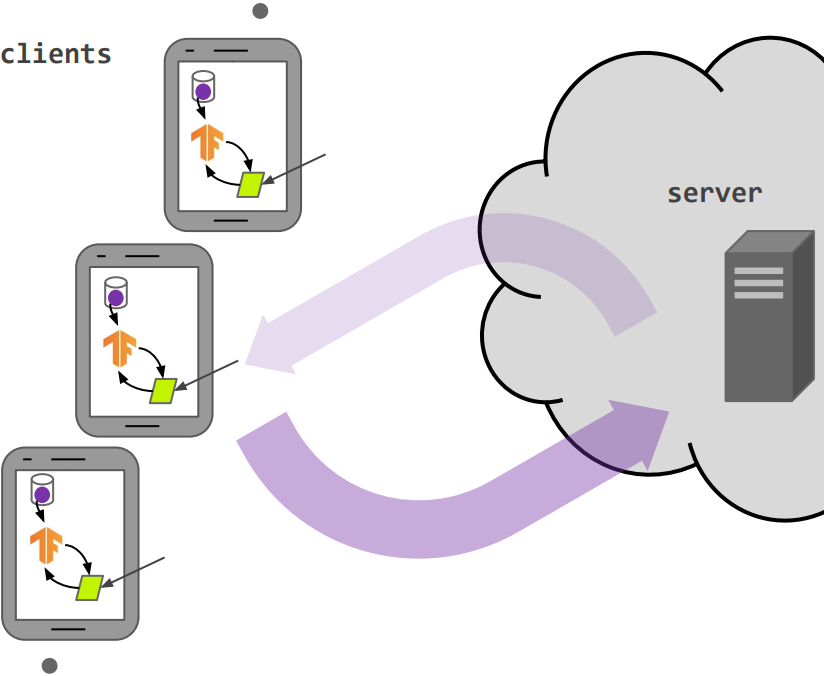
\includegraphics[width=0.7\textwidth]{Images/diagrams/FL_simplified.png}
        \decoRule
        \caption[FL system, simplified topology]{Simplified topology of an FL system \cite{survey_B}: \href{https://arxiv.org/abs/1912.04977}{URL}.}
        \label{fig: FL simplified topology}
\end{figure}

\section{Motivation}
Most FL research, to our knowledge, focuses on simulations and treats edge devices as black boxes; generally ignoring their nature and constrains. Taking in consideration the complexities of implementing ML on hardware, recent advancements in FL might be diminished or invalidated. The main motivation of this thesis is to identify, explore and possibly overcome the intrinsic conflicts that exist between FL and Artificial Neural Network (ANN) training in Field Programmable Gate Arrays (FPGA)s. % Such conflicts can be the batch size, where in FL tends to be minimized.

Instead of being incompatible, these two technologies may complement each other, which is worth investigating. Frequently in FL, transformations are applied on the generated ANN variables to reduce network utilization and enhance privacy. These transformations, which include quantization \cite{Mills2020}, adding Gaussian noise \cite{Wei2020} and others, tend to be spatially independent and could be implemented highly efficiently in hardware accelerators like FPGAs.

Finally, FL literature is almost devoid of wall-clock time examples. This thesis aims to provide a real world FL implementation that may be considered as a benchmark for future research. Furthermore, in order to be extendable and utilized in future works, the FL implementation is modular and platform independent.

\section{Scientific Contributions}
% The main focus of this thesis is combining FL training with FPGA based ANN implementations, while exploring and overcoming their inherent conflicts. Furthermore, it focus on the mostly unexplored FL setting of small client pools and its implicit difficulties. Finally, it provides a real world implementation of FL that can be used as a benchmark for future works. This FL implementation is agnostic of the ANN training implementation and can be used as a starting point for future works.
The main aim of this thesis is to explore the feasibility and efficiency of FL systems that employ FPGAs for the underlying training, focused on the edge setting. To achieve this, such a system was developed, thoroughly tested and benchmarked. Its components that can be utilized as starting points, examples or benchmarks of future works are as follows:
\begin{itemize}
    \item An FL system that is agnostic of the underlying ML model and training method. In the context of this work, it is employed with multiple ANNs of various types that are trained on CPU, GPU and FPGA. It can be easily modified to encompass other models and training implementations.
    \item A robustness analysis which focuses on the mostly unexplored FL setting of small client pools and its inherent difficulties.
    \item An FPGA-based implementation of training a CNN, that is optimized for the parameter space where the FL process is most efficient.
    \item Wall-clock timings of the CNN implementation and overall FL system, compared with equivalent implementations based on other technologies.
\end{itemize}
Finally, the aforementioned analyses and benchmarks are analyzed to provide apt suggestions for future works.

\section{Thesis Approach}
As the thesis moves forward, conflicts in terms of design and implementation are anticipated to arise between the two technologies. Furthermore, this is an mostly unexplored field. As such, a conservative and steady approach is expected to work best. 

Initially, a FL implementation that is agnostic and independent of the underlying training implementation, is developed. Its robustness is thoroughly validated, using TensorFlow to facilitate the local training. Subsequently, an FPGA-based CNN training implementation is created. 

Furthermore, an intermediate layer that connects the networking code of the FL clients with the FPGA driver is developed. With this approach, the FL implementation is combined with the FPGA-based implementation, and the overall system can be thoroughly tested and validated.

Finally, to benchmark the system, CPU and GPU implementation are developed and compared with it.

\section{Thesis Outline}
\begin{itemize}
    \item \textbf{Chapter 2 - Theoretical Background:} Description of the theoretical background of ML and FL.
    \item \textbf{Chapter 3 - Related Work:} Related works on FL, optimization techniques and hardware implementations of it.
    \item \textbf{Chapter 4 - FL architecture \& design:} Description of the FL architecture, design and implementation developed.
    \item \textbf{Chapter 5 - Robustness Analysis:} Analysis of the quality and performance of the FL implementation.
    \item \textbf{Chapter 6 - FPGA Implementation:} Description of the ANN architecture, design and implementation on FPGA developed.
    \item \textbf{Chapter 7 - Results:} Analysis of the quality and performance of the complete system. Comparisons with other technologies.
    \item \textbf{Chapter 8 - Conclusions and Related Work:} Conclusions and proposals for related future works.
\end{itemize}
\chapter{Theoretical Background}
\label{Chapter-Theoretical-Background}

%%%%%%%%%%%%%%%%%%%%%%%%%%%%%%%%%%%%%%%%%%%%%%%%%%%%%%%%%% Artificial Intelligence & Machine Learning %%%%%%%%%%%%%%%%%%%%%%%%%%%%%%%%%%%%%%%%%%%%%%%%%%%%%%%%%%
\section{Artificial Intelligence \& Machine Learning}
Various researchers and textbooks may provide different definitions of Artificial Intelligence (AI). Depending the school of though, AI is an artificial actor that thinks or acts, rationally or human-like, depending on what it knows. Generally, AI can be described as the study of intelligence agents. It is a modern science that encompasses a large variety of sub-fields, ranging from general-purpose areas, such as learning, to specific tasks like playing chess and giving medical diagnoses. AI can be relevant to any intellectual field, as it systematizes and automates intellectual tasks. \cite{russell_norvig_2003_1}

Machine learning (ML) is an AI field in which agents, in addition to the performance element, include a learning element that utilises their past experiences to enhance their behaviour. The core idea behind ML is that perception should be used to improve the ability to act in the future, not simply react in the present. Designing a learning element is a multi-facet problem that is affected by three major issues. \cite{russell_norvig_2003_18}

\subsection{Information management}%TODO:find a better title
The first issue is determining what information what information is useful and how it should be utilized. Different components of the input and output data should be learnt depending on the context in which the learning actor operates. One method is to directly link the current state of the actor or the world to their actions. Sometimes it can be more appropriate to infer relevant patterns from the data while ignoring unnecessary information. Another way is to collect action-value information indicating the desirability of actions based on their effect in the world state. These and other options may need to be combined in order to extract the most meaningful knowledge from the available data.

A common example is feature extraction. In ML, a feature \cite{Elgendy2020_ml_feature} is an individual measurable property or characteristic of a phenomenon being observed. They can be generic, such as edges in an image, or specialized, such as wheels and animal height. Feature extraction is the process of transforming such raw data into numerical features that can be processed.
\begin{figure}[H]
    \centering
        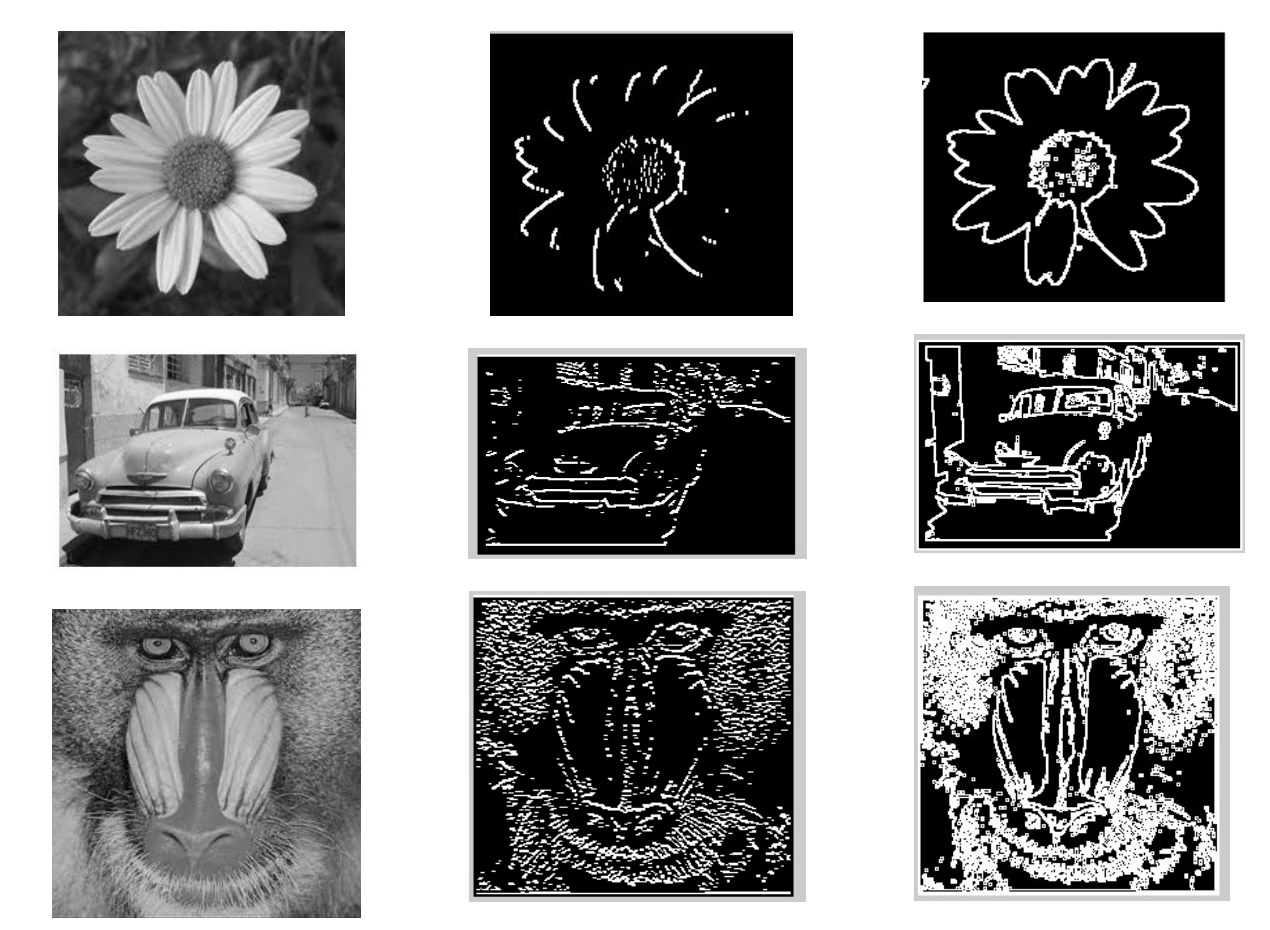
\includegraphics[width=0.8\textwidth]{Images/edge_detection.png}
        \decoRule
        \caption[Edge detection in greyscale images]{Edge detection in greyscale images: \href{https://aryamansharda.medium.com/how-image-edge-detection-works-b759baac01e2}{URL}.}
        \label{fig:Edge detection in greyscale images}
\end{figure}

Another key factor when designing learning systems is the availability of prior knowledge. Researchers have extensively looked into the issue where the agent uses only information that they encounter, but ways for transferring prior knowledge have been devised to speed up learning and improve decision-making.\cite{Transfer_Learning}

\subsection{Feedback mechanism}
The type of feedback available has a significant impact on the design and is perhaps the most crucial aspect of the learning problem. Usually three major types are distinguished: supervised, unsupervised, and reinforcement learning.

Supervised learning problems involve learning functions between sets of inputs and outputs. This is the case of a fully observable environments where the effects of the actors actions are immediately visible or the existence of a third party providing the correct solutions.

Unsupervised learning problems, on the other hand, do not supply output values and learning patterns are solely based on the input. As it has no knowledge of what constitutes a correct action or a desired state, an unsupervised learning agent cannot learn what to do. The hope is that through mimicry, the algorithm will generate imaginative content from it. This is a common scenario for probabilistic reasoning systems or when generating output data is prohibitively expensive. For the last case, a semi-supervised learning setting, in which only a subset of the outputs is generated, might be useful.

In the reinforcement learning setting there is no correct output provided, instead a reward is given to actor appropriate to the desirability of their actions. This is common when the world which the actor take part in continuously change according to their actions, or a desirable or undesirable state may be reached after a series of actions.

\subsection{Representation of the learned information}
The representation of the learned information is another important factor in establishing how the learning algorithm should operate. Common schemes include linear weighted polynomials for utility functions, propositional or first order logic, probabilistic representations like Bayesian Networks\cite{Probabilistic_Reasoning} and ANNs\cite{McCulloch1943}, and other methods have all been created.

%%%%%%%%%%%%%%%%%%%%%%%%%%%%%%%%%%%%%%%%%%%%%%%%%%%%%%%%%%%%%%%%%%%%%%%% Deep learning %%%%%%%%%%%%%%%%%%%%%%%%%%%%%%%%%%%%%%%%%%%%%%%%%%%%%%%%%%%%%%%%%%%%%%%%%
\section{Deep learning}
Deep learning is a sub-field of ML, partially overlapping with big data science. It consists of algorithms that use the perceptron as their basic building block, which is a mathematical function based on the McCulloch-Pitts model of biological neurons. They typically have hundreds of thousands to millions of perceptors with a variety of designs and topologies. Deep learning architectures include Deep Neural Networks (DNN)s, Convolutional Neural Networks (CNN)s, Recurrent Neural Networks (RNN)s and others, each one offering different capabilities and options.
\begin{figure}[H]
    \centering
        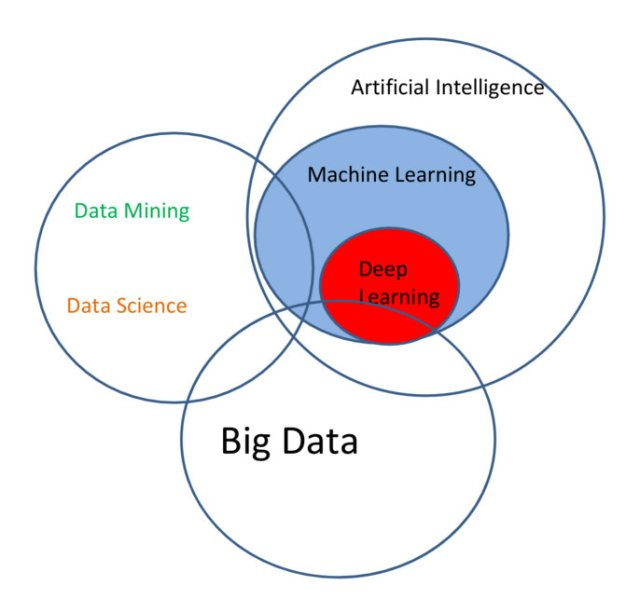
\includegraphics[width=0.6\textwidth]{Images/diagrams/ai_data_science.jpg}
        \decoRule
        \caption[AI Venn Diagram]{AI, ML, DL, Data Mining, Data Science, and Big Data: \href{https://whatsthebigdata.com/2016/10/17/visually-linking-ai-machine-learning-deep-learning-big-data-and-data-science/}{URL}.}
        \label{fig:AI Venn Diagram}
\end{figure}

Deep learning applications have demonstrated human-like or superior capabilities in several scientific and commercial fields such as image\cite{Alexnet} and speech\cite{limits_speech_recognition} recognition, natural language processing\cite{natural_language}, climatology\cite{Climatology} and biotechnology\cite{biotechnology}. Due to these exceptional capabilities and wide range of applications, deep learning has attracted a large number of researchers from various scientific domains, resulting in its tremendous expansion. However, the science is still young and there are a number of challenges to be overcome. Expecting deep learning combined with improved data processing being a solution to computers gaining generic human-like intelligence (human equivalent AI) is still a distant dream.\cite{dl_evolution}

Historically, the field of deep learning emerged in 1943 with the inception of the aforementioned McCulloch-Pitts perceptron. In 1949, Donald Hebb noted out in his book "The Organization of Behavior" that neural pathways are strengthened each time they are utilized, a principle that is crucial to how humans learn. He claimed that when two nerves fire at the same moment, the link between them is strengthened. This progress resulted in the creation of the first real-world application of ANNs, "MADALINE" an adaptive filter that eliminates echoes on phone lines. In 1962, Widrow \& Hoff developed a learning procedure that distributed the error across the ANN, resulting in its eventual elimination. Despite these advances, deep learning research plummeted due to a variety of internal and external factor, including the widespread use of fundamentally faulty learning function and the adoption of von Neumann architecture across computer science.

\begin{figure}[H]
    \centering
        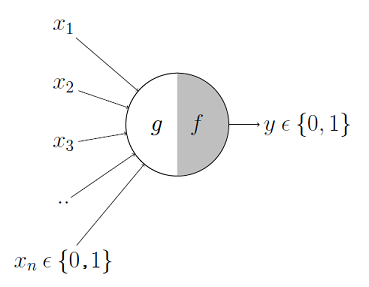
\includegraphics[width=0.6\textwidth]{Images/ANNArchitectures/McCulloch-Pitts Neuron.png}
        \decoRule
        \caption[McCulloch-Pitts Neuron]{The McCulloch-Pitts Neuron: \href{https://towardsdatascience.com/mcculloch-pitts-model-5fdf65ac5dd1}{URL}.}
        \label{fig:McCulloch-Pitts Neuron}
\end{figure}

Deep learning research stagnated until 1975, when developments such as Werbos' backpropagation and the building of the first multilayered network reignited interest in the field. Since then, the field continues to expand with innovations like hybrid models and ANN pooling layers. The current focus is on developing deep learning-specific hardware, as fast and efficient ANNs rely on it being defined for their use. Generally, architectures based on accelerators such as GPUs and FPGAs, or VLSI hardware-based designs, outperform CPU-based architectures. \cite{dl_history}

\subsection{Artificial Neuron}
As previously stated, the perceptron, also known as the artificial neuron, is the fundamental building element of the deep learning algorithms. In its simplest form, the artificial neuron receives one a set of inputs and sums it to produce an output. In practice, each input is weighted, then summed with a bias variable that acts as a threshold value, and the output is produced using an activation function.

The mathematical formula of the artificial neuron is defined as:
\begin{equation}
	y = \Phi( b + \sum_{i=1}^{I}x_i*w_i )
	\label{eqn:Artificial Neuron}
\end{equation}
Where:
\begin{conditions}
    y & output\\
    b & bias\\
    I & number of inputs \\
    \Phi & activation function\\
    w & weight
\end{conditions}

\subsection[Activation Functions]{Activation Functions \footnote{Also called transfer functions.}}
The activation function\cite{activation_function} of the artificial neuron is arguably its most important feature. It specifies how the weighted total of the inputs is transformed into an output (a target variable, class label, or score). Sometimes they limit their output range and are called squashing functions. There are various functions that are used as activation functions, with different properties and use cases each.

Most activation function are usually nonlinear so that the output varies nonlinearly with the inputs. With a linear activation function, regardless of how many layers a ANN has, it would behave just like a single-layer perceptron, as stacking linear functions creates just another linear function. Nonlinearity is, arguably, the most important aspect of the activation functions.

Activation functions are usually differentiable, which means that for a given input value, the first-order derivative can be determined. This is necessary because ANNs are mostly trained using the backpropagation of error algorithm, which requires the derivative of prediction error to update the model's parameters.

\subsubsection{Binary Step}
This is arguably the most basic activation function, as it was originally used in the McCulloch-Pitts Neuron and operates like a simple threshold. It activates the output of the perceptron when a certain value is exceeded, else the output is set as zero.
\begin{equation}
	f \left( x \right) = \left\{
    	\begin{array}{ll}
    	    0 & x \leq threshold\\
    	    1 & x > threshold\\
    	\end{array} 
	\right.
	\label{eqn:Binary step}
\end{equation}

\subsubsection{Sigmoid}
Also known as the logistic function, it normalizes and squashes the output of the neuron between 0 and 1. Its most important properties are that the output is barely affected by extreme values and the derivative is easily calculated.
\begin{equation}
	f \left( x \right) = \frac{1}{1+e^{-x}}
	\label{eqn:Sigmoid}
\end{equation}

\subsubsection{ReLU}
Because of its simple implementation, non-linearity, and high performance, the Recti-Linear Unit or ReLU function is arguably the most commonly utilized function in ANNs. It combines the binary step function for negative values and the identity function for positive values.
\begin{equation}
	f \left( x \right) = \left\{
    	\begin{array}{ll}
    	    0 & x \leq 0\\
    	    x & x > 0\\
    	\end{array} 
	\right.
	\label{eqn:ReLU}
\end{equation}

\subsubsection{Softmax}
Softmax ensures that all the outputs sums to 1 by normalizing them to a probability distribution. As such, it is mostly used as the final activation function in multi-decision ANN models.
\begin{equation}
	f \left( x \right)_{i} = \frac{e^{x_i}}{\sum_{k=1}^{K}e^{x_{j}}}
	\label{eqn:Softmax}
\end{equation}

\subsection{Artificial Neural Network architectures}
ANNs are collections of artificial neurons, typically organized in layers. Different layers may utilize different activation functions and/or apply different transformations to their inputs. Generally, the outputs of one layer's neurons are connected with the inputs of the following layer's neurons. If this holds true for all neurons in the ANN, the ANN is "fully connected". Alternatively, connections can be sparser, or loops between one or more layers can be created, giving the ANN different traits and capabilities.

When designing a layer, its position in the ANN is probably one of the most important variables. The input layer is the layer that accepts external data and is significantly dependent on the structure of the input; text input requires quite different management than visual input. The output layer is the layer that generates the final result, and its primary design factor is the nature of the output, which can be a yes or no answer, a classification or a set of probabilities. Usually, in order to have a human-readable output, specialized activation functions like softmax are used.

\subsubsection{Deep Neural Network (DNN)}
Between the input and output layers, there can be zero or more "hidden" layers. Typically, the majority of the network's computation takes place in these layers, and their design is influenced by a variety of criteria such as the nature of the problem and the input, available processing resources, and the required minimum capabilities. A DNN is defined as a ANN that has multiple hidden layers.\cite{IBM_Neural_Networks}
\begin{figure}[H]
    \centering
        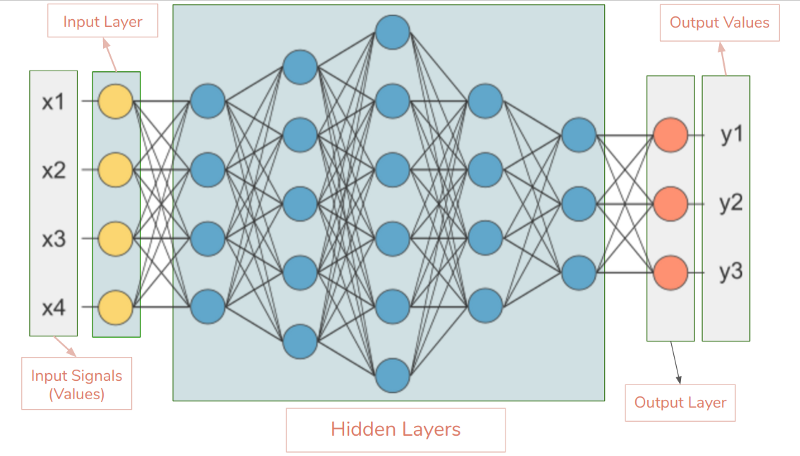
\includegraphics[width=0.8\textwidth]{Images/ANNArchitectures/dnn.png}
        \decoRule
        \caption[Deep neural network]{DNN with 5 hidden layers: \href{http://www.gabormelli.com/RKB/Multi_Hidden-Layer_(Deep)_Neural_Network}{URL}.}
        \label{fig:Deep neural network}
\end{figure}

\subsubsection{Convolutional Neural Network (CNN)}
The introduction of CNNs\cite{CS231n_stanford_cnn} is arguably one of the most significant achievements in the field of Deep Learning. They excibit great performance in image and video recognition, recommender systems, image classification, image segmentation, medical image analysis, natural language processing, brain-computer interfaces, and computer vision, among other applications. They perform best when the input is an image or a succession of images, but they are also effective in other scenarios.

CNNs are distinguished by their use of convolutional and subsampling layers, which enable the creation of multiple filters that can be trained in parallel. These filters are utilized to isolate and extract features from input data that would be undetectable by simpler DNNs. Subsequently, in order to get a result, the output of these filters is fed to fully connected layers. The design and depth of these filters are directly responsible for the network's feature extraction capabilities.

\begin{figure}[H]
    \centering
        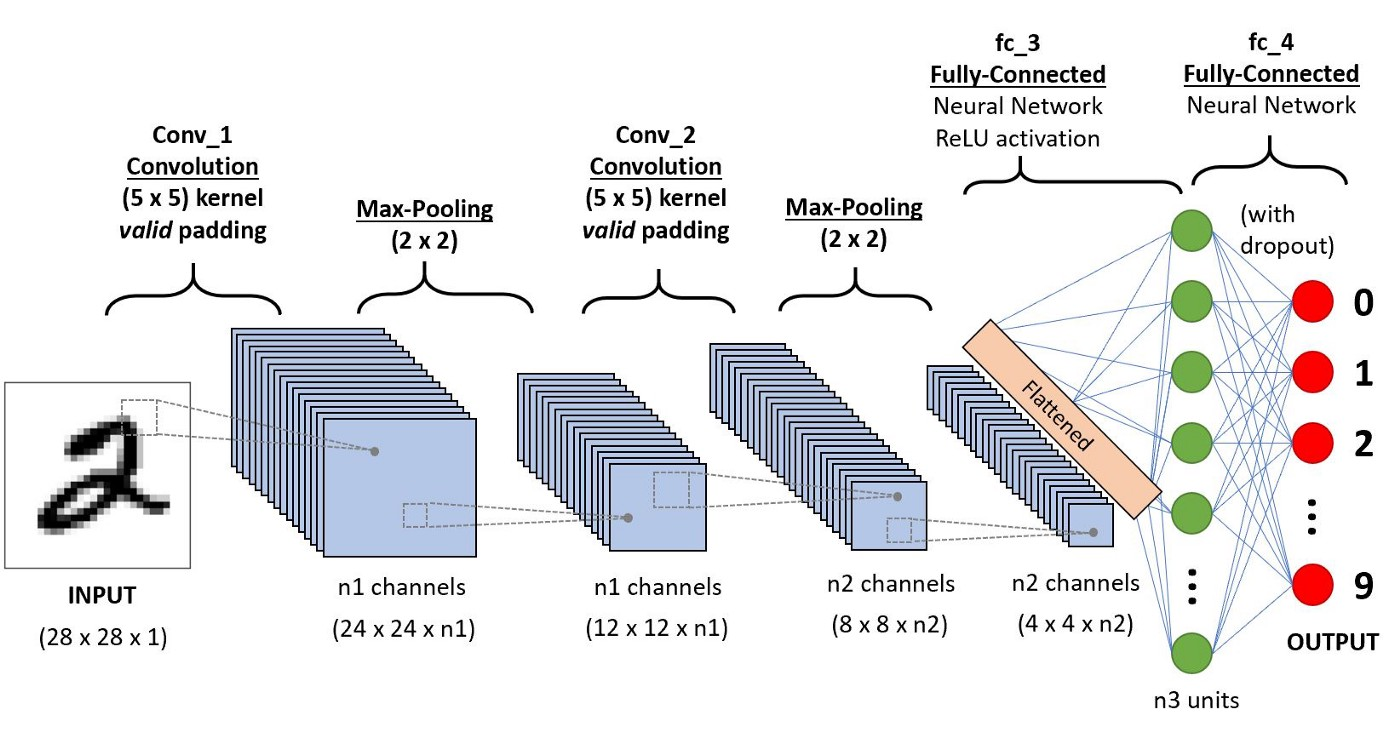
\includegraphics[width=1\textwidth]{Images/ANNArchitectures/cnn_2conv_layers.jpg}
        \decoRule
        \caption[A CNN sequence to classify handwritten digits]{A CNN sequence that classifies handwritten digits using 2 convolutional layers: \href{https://towardsdatascience.com/a-comprehensive-guide-to-convolutional-neural-networks-the-eli5-way-3bd2b1164a53}{URL}.}
        \label{fig:A CNN sequence to classify handwritten digits}
\end{figure}

Convolutional layers carry out the convolution process with the help of small matrices known as kernels. The kernel is the beating heart of a layer, and its type and dimensionality determine how the layer functions. Typically, two-dimensional kernels are used, while their size is mainly depended on the size of the input and their position on the network. A single convolutional layer can usually only produce filters that detect generic low-level features, such as edges and color. In order to create more specialized filters that can detect high-level features, multiple layers are used.

\begin{figure}[H]
    \centering
        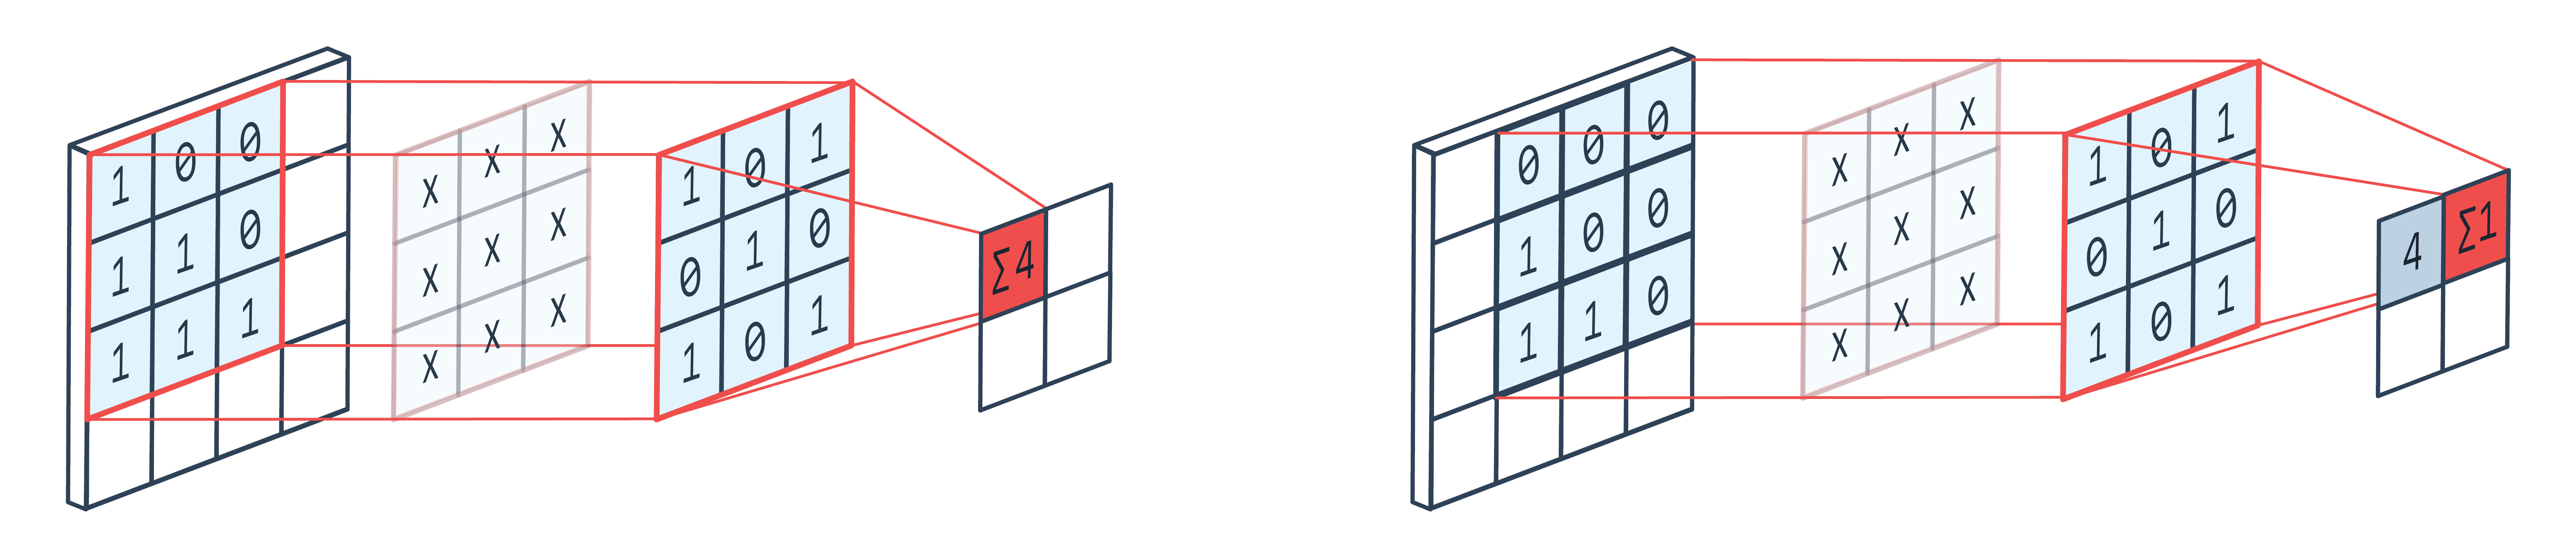
\includegraphics[width=1\textwidth]{Images/ANNArchitectures/2d_convolution.png}
        \decoRule
        \caption[2D convolution]{2D convolution: \href{https://peltarion.com/knowledge-center/documentation/modeling-view/build-an-ai-model/blocks/2d-convolution}{URL}.}
        \label{fig:2D convolution}
\end{figure}

The subsampling layers is the second distinguishing innovation of CNNs. Their primary task is to enable the network to recognize features without relying on their exact location. Furthermore, they simplify the network by reducing its number of parameters. Typically, they immediately follow convolutional layers in order to decrease the size of the features. Common subsambling layers include max pooling, mean pooling and others.

\begin{figure}[H]
    \centering
        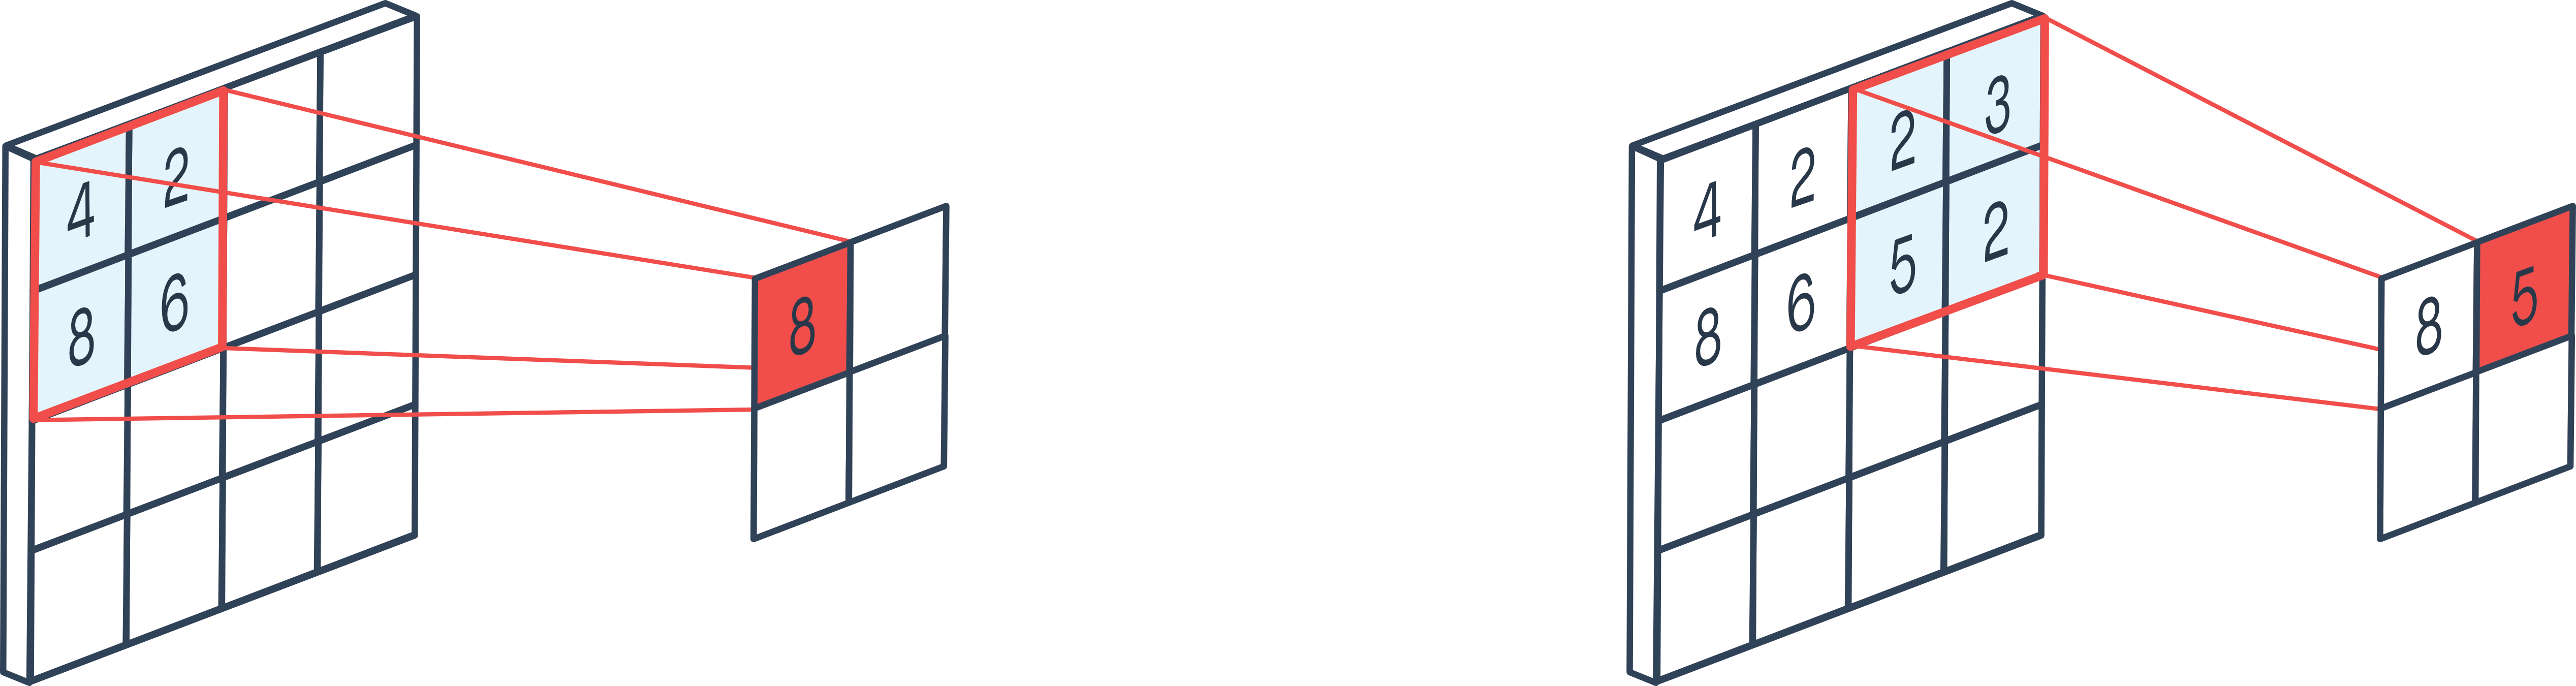
\includegraphics[width=0.76\textwidth]{Images/ANNArchitectures/2d_max_pooling.png}
        \decoRule
        \caption[2D max pooling]{2D max pooling: \href{https://peltarion.com/knowledge-center/documentation/modeling-view/build-an-ai-model/blocks/max-pooling-2d}{URL}.}
        \label{fig:2D max pooling}
\end{figure}

% \subsubsection{rnn?}

\section{Training Artificial Neural Networks}
As previously stated, ANNs are made up of neurons, which contain multiple parameters known as weights and biases, which are generally referred simply as weights. Training\footnote{Also called fitting.} is an iterative process that aims to improve the ANN's performance by optimizing these parameters. To accomplish this, three key elements are required: a loss function, an optimization algorithm such as gradient descent and a training algorithm like backpropagation.

In supervised learning, input-output examples are fed to the ANN. It produces predictions based on the inputs and then uses the loss function to compare these predictions to the intended outputs. The loss function calculates the ANN's error, which is a quantifiable difference between the expected and actual output. The error gradients of the ANN's weights are then determined, commonly using the backpropagation process. Finally, the optimization algorithm uses the error gradients to generate new values for the weights that should perform better.

In unsupervised learning, only input examples are given. The ANN attempts to mimic the data it is given and optimizes itself using the mistake in its output. Instead of a loss function, the error is represented as the likelihood of an incorrect output. The error gradients can be computed using a variety of learning algorithms, such as Maximum Likelihood, Maximum A Posteriori, and others, rather than the predominantly used backpropagation in supervised learning. Finally, to generate new values for the ANN's weights, any optimization algorithm may be employed.

In reinforcement learning, the ANN produces a prediction and subsequently receives a feedback\footnote{Feedback is frequently given after a series of predictions.}, usually numerical, regarding its performance. The loss function uses this feedback and prediction, and like in the supervised learning, the error gradients are calculated through backpropagation. Finally, the ANN's weights are updated using a optimization algorithm.

The training technique varies greatly depending on the problem, the ANN architecture, and numerous other factors, but it is always iterative. An epoch is typically defined as using all of the data points in the training set once.

\subsection{Initialization}
The initialization of the ANN's weights has a significant impact on the ANN's final performance and training time. Naive methods, such as zeroing all weights or assigning them fully random values, might produce detrimental effects. If the weights in a ANN start out too small, the signal will shrink as it passes through each layer, eventually becoming too small to be useful. Likewise, if the weights in an ANN start out too large, the signal grows too huge as it goes through the layers, eventually overwhelming all other signals. As a result, the ANN may require a significant amount of training time or possibly become stuck in its initial state and not converge to a solution.

One common ANN initialization scheme used to solve this problem is called Glorot\footnote{also known as Xavier. \cite{Xavier_initialization}} Initialization\cite{pmlr-v9-glorot10a, Glorot_initialization_large}. The idea is to initialize each variable with a small Gaussian value with mean of 0 and variance based on its fan-in and fan-out\footnote{In a fully connected ANN, the fan-out of a layer equals the fan-in of the next layer.}. The Glorot Initialization not only outperforms uniform random initialization (in most circumstances), but it also eliminates the need to determine appropriate fixed limit values. There are actually two versions of Glorot initialization, Glorot uniform and Glorot normal, with different distribution and variance.

The variance of the Glorot Initialization is defined as:

\noindent\begin{minipage}{.5\linewidth}
    \begin{equation}
    	V \left[ W_i \right] = \frac{2}{n_i+n_{i+1}}
    	\label{eqn:Glorot Initialization variance, uniform distribution}
    \end{equation}%
    \captionof*{figure}{Uniform distribution}
\end{minipage}%
\noindent\begin{minipage}{.5\linewidth}
    \begin{equation}
    	V \left[ W_i \right] = \frac{\sqrt{6}}{\sqrt{n_i + n_{i+1}}}
    	\label{eqn:Glorot Initialization variance, normal distribution}
    \end{equation}
    \captionof*{figure}{Normal distribution}
\end{minipage}
Where:
\begin{conditions}
    V & variance\\
    i & layer\\
    W & weights\\
    n & fan-in of a layer\\
\end{conditions}

The Glorot initialization makes the assumption that the activations immediately after initialization are linear, as the initialized values are close to zero and their gradients close to 1. While this holds true for the traditional activation function its development was based on\footnote{Sigmoid, tanh and softsign.}, it is invalid for the more modern rectifying nonlinearities\footnote{ReLU and PReLU.} in which the non-linearity is at zero. As such, the He Initialization \cite{He_Init_paper, Glorot_He_initialization} was proposed, with Gaussian distribution and the following variance:
\begin{equation}
	V \left[ W_i \right] = \frac{2}{n_i}
	\label{eqn:He Initialization variance}
\end{equation}


\subsection[Loss Functions]{Loss Functions \footnote{Also called cost or error functions.}}
A loss function\cite{loss_functions} provides a real number that represents the error a function associated with an event. In Deep Learning, it quantifies the inaccuracy of a ANN. The training algorithm tries to minimize this number by altering the ANN's weights, in hopes that it improves the network's accuracy. The choice of loss function is influenced by the nature of the input, as well as by the nature of the output. Some of the most common loss functions are listed below.

\subsubsection{Regression Loss Functions}
Regression problems involve predicting numerical values, a number or set of numbers. This is a usual problem in supervised learning. The appropriate loss functions measure the distance between the prediction and the ideal values.

The most frequent regression loss function is Mean Squared Error (MSE). This method is utilized when the prediction belong to a continuous plane. The MSE is the mean of the squared distances between the predicted values and the target variables.
\begin{equation}
    	Loss = \frac{ \sum_{i=1}^{n} \left( y_i^{target} - y_i^{pred.} \right)^2 } {n}
    	\label{eqn:Mean Squared Error}
\end{equation}

When the data are discrete values, the Poisson loss function is more appropriate. Under the assumption that the target comes from a Poisson distribution, minimizing the Poisson loss is equivalent of maximizing the likelihood of the data.
\begin{equation}
    	Loss = \frac{1}{N} \sum_{i=0}^{N} \left( y_i^{pred.} - y_i^{target}\log y_i^{pred.} \right)
    	\label{eqn:Poisson Error}
\end{equation}

\subsubsection{Classification Loss Functions}
In classification problems, the examples must be classified into one or more classes, which may or may not be preset. The ANN generates a probability distribution that represents its confidence in the example's classification.

Binary cross-entropy is a loss function that is used in binary classification tasks with predefined classes. These are tasks that answer a question with only two choices.
\begin{equation}
    	Loss = - 
    	\frac{1}{ \substack{ output\\ size } }
    	\sum_{i=1}^{ \substack{ output\\ size } }
    	y_i^{target} \cdot \log y_i^{pred.} + 
    	\left( 1 - y_i^{target} \right) \cdot
    	\log \left( 1 - y_i^{pred.} \right)
    	\label{eqn:Binary cross-entropy}
\end{equation}

In problems with more than one classes, the categorical cross-entropy loss function, a generalization of binary cross-entropy loss function, is most commonly used. The \( y_i^{target}\) is the probability that event \( i \) occurs and the sum of all these probabilities is 1, meaning that exactly one event may occur.
\begin{equation}
    	Loss = 
    	- \sum_{i=1}^{ \substack{ output\\ size } }
    	y_i^{target} \cdot \log y_i^{pred.}
    	\label{eqn:Categorical cross-entropy}
\end{equation}

Classification problems in unsupervised learning is quite different, as the desired output is not provided to the ANN. The most commonly used training algorithm is k-means clustering. It aims to partition the examples into a predefined number of clusters. To achieve this it tries to minimize the pairwise squared deviations of points in the same cluster. The equivalent to a loss function is defined as:
\begin{equation}
	\argmin_S \sum_{i=1}{k} \frac{1}{ \left| S_i \right| } \sum_{}{x,y \in S_i} \left\| x-y \right\|^2
	\label{eqn:k-means error}
\end{equation}
Where:
\begin{conditions}
    S & clusters\\
    x,y & points in cluster\\
\end{conditions}

\subsubsection{Reward Functions}
Reward functions serve the same goal as loss functions in that they quantify the accuracy of an ANN in order to optimize it, but in the opposite direction. Rather than penalizing the ANN, it rewards it based on its performance, with the learning algorithm aiming to maximize this reward. This is most frequently seen in Reinforcement Learning. Reward functions specify how the agent should behave, hence their structure is heavily influenced by the problem and the laws of the universe in which the agent lives. 

\subsection{Backpropagation}
Backpropagation\cite{backpropagation_original, Backpropagation_wiki} is a training algorithm for feedforward ANNs under supervised learning\footnote{Generalizations of the algorithm can be used for other network architectures and different training schemes.}. Feedforward ANNs refers to fully connected networks with no cyclical connections, most DNNs and CNNs adhere this standard. For a single example, backpropagation computes the gradient of the loss function with respect to the network weights. The gradient\cite{gradient_wiki} represent the direction and rate of fastest rise. If a function's gradient is non-zero at a point, the gradient's direction is the direction in which the function increases the fastest, and the magnitude of the gradient is the rate of growth in that direction, in respect of that point.

Backpropagation is sometimes misconstrued to mean the entire learning algorithm for ANNs. Backpropagation is merely the method for computing the gradient; another algorithm, such as stochastic gradient descent, is needed to accomplish learning using this gradient. Furthermore, backpropagation is frequently misinterpreted as being limited to ANNs while, in fact, it may compute derivatives of any function. Its use to ANNs is critical because it enables efficient training, especially when using hardware accelerators.

The ANN can be mathematically expressed as:
\begin{equation}
    g \left( x \right) \coloneqq f^L \left( W^L f^{L-1} \left( W^{L-1} \cdots f^1 \left(  W^1 x \right) \cdots \right) \right)
	\label{eqn:Feedforward ANN definition}
\end{equation}
Where:
\begin{conditions}
    x & input\\
    g(x) & prediction\\
    f^l & activation functions at layer \(l\)\\
    W^l & weights at layer \(l\)\\
    L & number of layers\\
\end{conditions}

Then the error function \(C\) with desired output \(y\) is:
\begin{equation}
    C \left( y , 
    f^L \left( W^L f^{L-1} \left( W^{L-1} \cdots 
    f^1 \left(  W^1 x \right) \cdots \right) \right) 
    \right)
	\label{eqn:Backpropagation, loss function}
\end{equation}

By using the chain rule the total derivative of the loss function is:
\begin{equation}
    \frac{\mathrm{d}C}{\mathrm{d}y} \circ 
    \left( f^L \right)' \cdot W^L 
    \circ \left( f^{L-1} \right)' \cdot W^{L-1} \cdots 
    \left( f^{1} \right)' \cdot W^{1}
	\label{eqn:Backpropagation, total derivative of the loss function}
\end{equation}

Given that the gradient \(\nabla \) in respect to the input is the transpose of the derivative in respect to the output, the total gradient can be determined as:
\begin{equation}
    \nabla_x C =
        \left( W^{1} \right)^T \cdot \left( f^{1} \right)' \cdots \circ
        \left( W^{L-1} \right)^T \cdot \left( f^{L-1} \right)' \circ
        \left( W^{L} \right)^T \cdot \left( f^{L} \right)' \circ
        \nabla_y C
	\label{eqn:Backpropagation, total gradient}
\end{equation}

The partial gradients at each layer\( \delta^l \), which represent the effect of the weights in the corresponding layers on the error function, may be easily determined by eliminating the effect of the previous ones:
\begin{equation}
    \begin{split} 
        \delta^{1} & = 
            \left( f^{1} \right)' \circ 
            \left( W^{2} \right)^T \cdot \left( f^{2} \right)' \cdots \circ
            \left( W^{L-1} \right)^T \cdot \left( f^{L-1} \right)' \circ
            \left( W^{L} \right)^T \cdot \left( f^{L} \right)' \circ
            \nabla_y C\\
        \delta^{2} & =
            \left( f^{2} \right)' \cdots \circ
            \left( W^{L-1} \right)^T \cdot \left( f^{L-1} \right)' \circ
            \left( W^{L} \right)^T \cdot \left( f^{L} \right)' \circ
            \nabla_y C\\
        \delta^{L-1} & =
            \left( f^{L-1} \right)' \circ
            \left( W^{L} \right)^T \cdot \left( f^{L} \right)' \circ
            \nabla_y C\\
        \delta^{L} & =
            \left( f^{L} \right)' \circ
            \nabla_y C\\
    \end{split}
	\label{eqn:Backpropagation, per layer gradient}
\end{equation}

A naive approach would be to compute these derivatives forward. Backpropagation, on the other hand, eliminates duplicate multiplications by employing dynamic programming, as the derivative of one layer can be used to calculate the derivative of the previous one. Furthermore, by going backwards, a vector \(\delta^l\) is multiplied by exactly one matrix \(\left( W^{l} \right)^T \circ \left( f^{L-1} \right)'\) at each step. When calculating forwards, however, each multiplication multiplies a matrix with \( L-l \) matrices, which is a far more expensive operation.

\subsection{Gradient Descent}
Gradient descent\cite{IBM_Gradient_Descent, gradient_descent_wiki} is an optimization algorithm which is commonly used to train ANNs. Gradients generated by training algorithms such as backpropagation are used to alter the network's weights, in order to produce the minimal possible error. Its basis is that a differentiable function \(F\) decreases fastest at a point \(a_n\), in the direction of the negative gradient of that point \(-\nabla F \left( a_n \right)\). Mathematically it is defined as:
\begin{equation}
a_{n+1} = a_n - \gamma \nabla F \left( a_n \right)
	\label{eqn:Gradient Descent}
\end{equation}

The learning rate parameter \(\gamma\) is the size of the step taken each time the algorithm is executed. It has a significant impact on the overall performance of the training procedure and should be fine-tuned. If it is too large, there is a high risk of overshooting the minimum of the function. If it is too small, more iterations are needed, and there is a risk too end up in a suboptimal local minimum.
\begin{figure}[H]
    \centering
        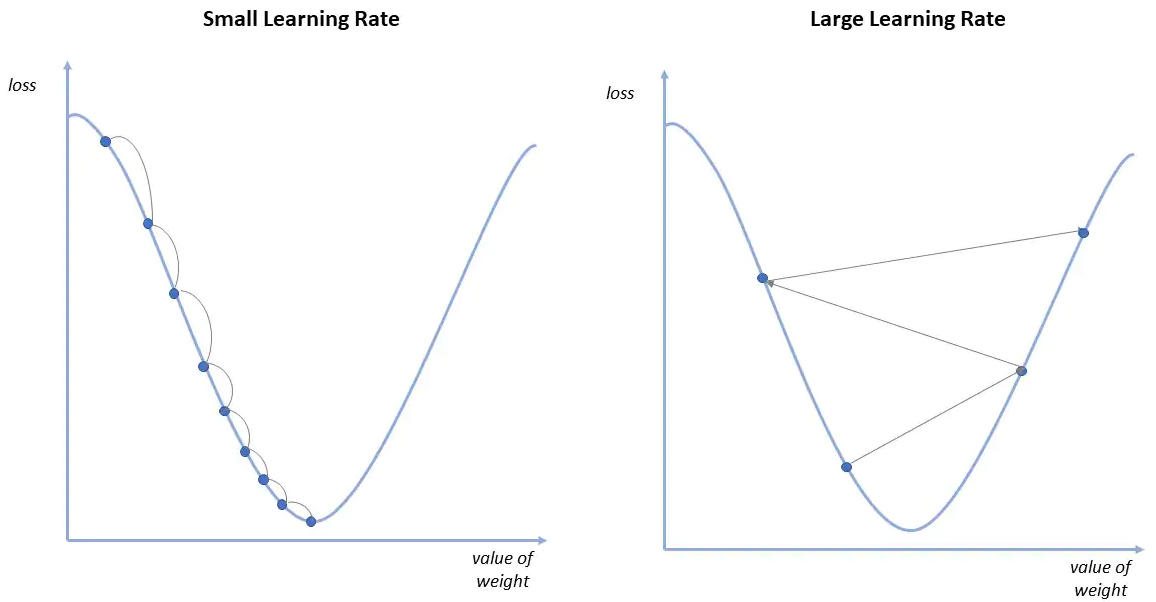
\includegraphics[width=0.8\textwidth]{Images/diagrams/learning_rate.png}
        \decoRule
        \caption[Effect of learning rate in Gradient Descent]{Effect of learning rate in Gradient Descent: \href{https://www.ibm.com/cloud/learn/gradient-descent}{URL}.}
        \label{fig:Learning rate in Gradient Descent}
\end{figure}

\subsubsection{Challenges}
Gradient descent faces challenges with local minima and saddle points, when the gradient gets close to zero the algorithm is unable to re-adjust the network's weights. Local minima resemble the global minimum in shape, trapping the algorithm. Saddle points are stable positions with no relative maximum or minimum, making it difficult for the algorithm to decide what to do.
\begin{figure}[H]
    \centering
        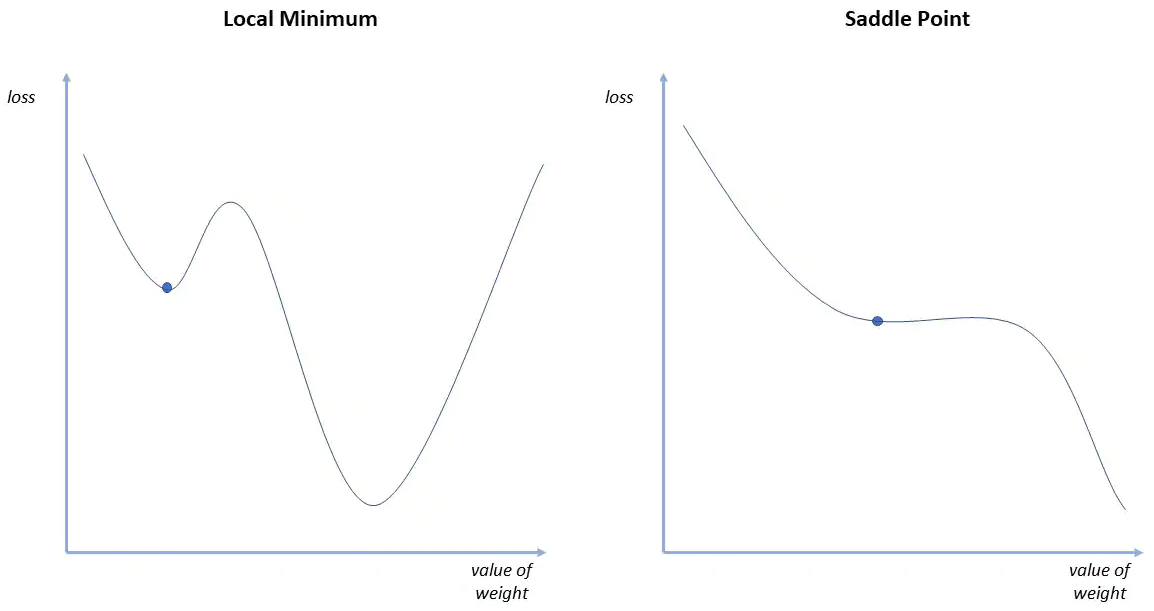
\includegraphics[width=0.8\textwidth]{Images/diagrams/LocalMinimum_SaddlePoints.png}
        \decoRule
        \caption[Local minimum and saddle point]{Local minimum and saddle point: \href{https://www.ibm.com/cloud/learn/gradient-descent}{URL}.}
        \label{fig:Local minimum and saddle point}
\end{figure}

To address this issue, a number of enhancements have been developed culminating in the Nesterov Momentum\cite{nesterov_momentum} extension. To accelerate the process, the first adjustment is to add a momentum variable, a percentage \(\beta\) of the previous iterations' change \(m\). Simply adding that tends to result in overshooting. To mitigate this, the calculation of the gradient takes the momentum of the previous steps into account. With Nesterov momentum, the gradient descent is defined as:
\begin{equation}
    \begin{gathered} 
        m_{n+1} = \beta m_n - \gamma \nabla F \left( a_n + \beta m_n \right)\\
        a_{n+1} = a_n + m_{n+1}\\
    \end{gathered}
	\label{eqn:Gradient Descent with Nesterov momentum}
\end{equation}

In deep ANNs with numerous or repeating hidden layers, training with backpropagation and gradient descend introduce the phenomenon of vanishing gradients. As the algorithm travels backwards through the layers, the gradients get smaller and smaller, eventually becoming insignificant and unable to alter the weights of the network. Non monotonic activation functions, such as ReLU, and more complex topologies, such as residual ANNs, are prevalent but not exclusive solution.

Another problem, especially frequent in RNNs, is exploding gradients. This occurs when a gradient gets too large, turning the model unstable. To address this, techniques such as dimensionality reduction have been developed, with the goal of reducing the model's overall complexity.

\subsubsection{Variations}
In vanilla Gradient Descent, each example's error is assessed, the gradients are produced and then the weights of the ANN are updated. In order to calculate the error of an example, the update of the prior one must be applied first. Since this process cannot be parallelized and must be repeated for each example, it is computationally inefficient.

Furthermore, the dataset is often used multiple times during the training of a model. In vanilla Gradient Descent, the examples are used in order. This pattern is often recognized by the models, which then introduce biases that lead to less-than-ideal solutions.

To address these inefficiencies, three key variations have been developed:

\begin{itemize}
    \item Batch Gradient Descent
\end{itemize}
Batch gradient descent performs backpropagation and updates the network only after calculating the loss function for \textit{all} the examples in the training dataset. The expensive operations of calculating the gradients and new weights occur just once per epoch, resulting in a computationally more efficient algorithm. Furthermore, the loss function can be parallelized indefinitely.

This method yields a stable error gradient and convergence, but it frequently leads to local minima. Furthermore, in order to calculate the loss, all of the data must be in memory, making the approach unsuitable for huge datasets. Finally, more passes through the dataset are needed, as updates are infrequent.

\begin{itemize}[resume]
    \item Stochastic Gradient Descent (SGD)
\end{itemize}
SGD works similarly to vanilla Gradient Descent, with the exception that the training examples are chosen at random. This eliminates the bias produced by consuming the examples in a particular order. Furthermore, its frequent updates produce noisy gradients, which aid in avoiding local minima.
    
\begin{itemize}[resume]
    \item Mini-batch Stochastic Gradient Descent
\end{itemize}
Mini-batch SGD builds on the ideas of the previous variations by splitting the training dataset randomly into small batches and performing updates on each one of them. This method achieves a balance between the computational efficiency of batch gradient descent and the randomness of SGD. This is by far the most popular variation, and it is commonly abbreviated just as SGD.

\subsection{Model Overfitting}
The goal of training ANNs is to improve their performance on real-world data, i.e. to generalize its knowledge. When training, the model\footnote{Most statistical models, not just ANNs, exhibit this phenomenon.} may sometimes fit exactly against training data, severely limiting its effectiveness with previously unseen data and negating its objective.

Training is typically conducted with a sample dataset. If the model trains on this for too long, or if the model is overly sophisticated, it may memorize irrelevant information, the "noise" within the training dataset. This is known as overfitting\cite{IBM_overfitting}, and the most common signs are unusually high accuracy on the training dataset and high variance within the predictions of the network.
\begin{figure}[H]
    \centering
        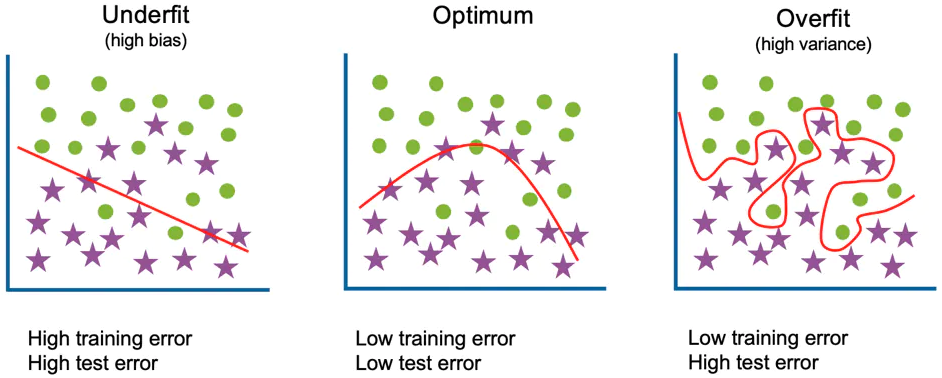
\includegraphics[width=1\textwidth]{Images/diagrams/model-over-fitting.png}
        \decoRule
        \caption[Model overfitting]{Model overfitting and its opposite, model underfitting: \href{https://www.ibm.com/cloud/learn/overfitting}{URL}.}
        \label{fig:Model overfitting}
\end{figure}

Multiple methods to avoid or suppress overfitting have been developed, some common ideas are listed below:
\begin{itemize}
    \item Early stopping
\end{itemize}
This method aims to stop the training before the model starts learning the noise within the model. To achieve this, a portion of the training dataset is held aside for testing rather than being used during training. This dataset is used to evaluate the ANN after each epoch, and if the accuracy is lower than before, training is terminated. There is a risk of stopping too soon and underfitting the model; a middle ground should be sought.
\begin{figure}[H]
    \centering
        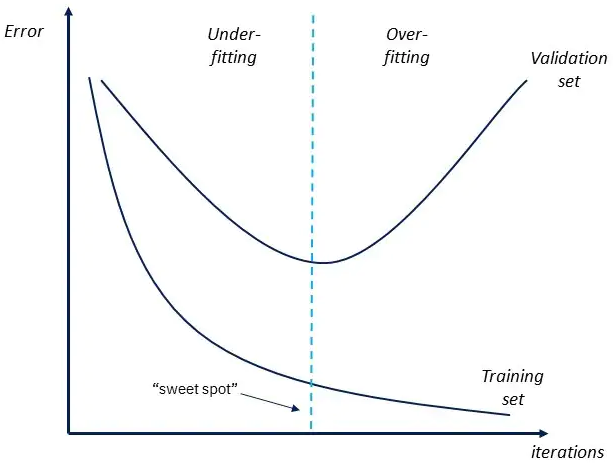
\includegraphics[width=0.6\textwidth]{Images/diagrams/classic_overfitting.png}
        \decoRule
        \caption[Overfitting/Underfitting]{Border between overfitting and underfitting: \href{https://www.ibm.com/cloud/learn/overfitting}{URL}.}
        \label{fig:Model Overfitting/Underfitting}
\end{figure}

\begin{itemize}[resume]
    \item Data manipulation
\end{itemize}
A common way to reduce overfitting is through manipulating the input data. Expanding the training dataset with real-world or machine-generated data can assist the model in identifying patterns between the input and output variables. When using clean and relevant data, this strategy is effective; otherwise, the model may grow too complex and overfit even more. Another technique is augmenting already existing data by adding noise to them. The goal is to help the model discern between useful and irrelevant patterns.

\begin{itemize}[resume]
    \item Model simplification
\end{itemize}
Multiple methods attempt to enhance the model's performance by simplifying it and the problem that is called to solve. Feature selection refers to a class of methods that enhance the training dataset by removing examples. Such methods include removing highly correlated features and incomplete examples, selecting the best features through statistical methods and others. Another family of methods, such as the Principle Component Analysis, seek to transform the features by reducing their dimension.

The preceding methods necessitate some level of domain knowledge, which is not always available. In this scenario, regularization methods are particularly helpful, as they aim to reduce complexity by altering the model. In general they try to penalize input parameters with large coefficients, typical in examples with significant noise, in order to minimize the variance in the model. Such methods include L1 regularization, dropout and others.

% \subsection{Adaptive Learning Rate?}
% \subsection{Adaptive algoritms?}
%%%%%%%%%%%%%%%%%%%%%%%%%%%%%%%%%%%%%%%%%%%%%%%%%%%%%%%%%%%%%%%%%%%%%% Federated learning %%%%%%%%%%%%%%%%%%%%%%%%%%%%%%%%%%%%%%%%%%%%%%%%%%%%%%%%%%%%%%%%%%%%%%
\section{Federated Learning}
%definition and central aim
Federated Learning \cite{FL-original-paper, FL_comprehensive_survey} (FL) is a ML setting in which multiple clients, ranging from big enterprises to personal mobile devices, collaborate to train a model under the supervision of a central server. The goal of this is to alleviate many of the systemic privacy problems associated with centralization by decentralizing the training data. Under FL, any model that employs SGD-like approaches can be trained. ANNs, linear regression, Support Vector Machines, and other models fall into this category. FL acts as a wrapper for ML; what is true for a model when trained locally tends to hold true when trained in a FL context.

% basic entities and operation
In general, the FL setting has two basic entities: data owners (participating clients) and model owners (orchestrating server). Participants never share their datasets, instead use them to locally train a model sent by the orchestrating server. The generated weights are shared, which the server aggregates them in order to construct a global model. The models trained by the clients are referred as local models whereas the aggregated model is referred as global model.

% basic topology
The entities are typically configured in a hub-and-spoke topology, as shown in figure \ref{fig:FL topology}, with the hub representing the coordinating server and the spokes connecting to the clients. The server organizes the training but never access the training data.
\begin{figure}[H]
    \centering
        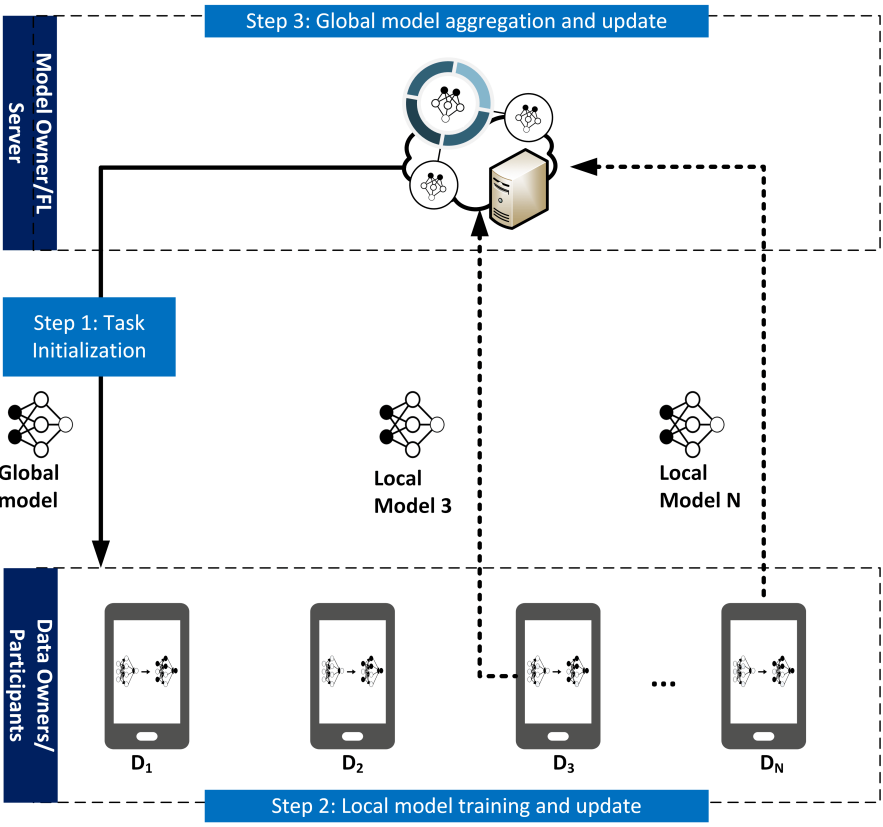
\includegraphics[width=0.6\textwidth]{Images/topologies/fl_topology.png}
        \decoRule
        \caption[FL topology]{Typical FL topology: \href{https://ieeexplore.ieee.org/document/9060868}{URL}.}
        \label{fig:FL topology}
\end{figure}

% operation/ basic loop
\subsection{Typical Federated Training Process}
FL training is a continuous process. Each iteration is referred as a global epoch and can be broken down into three main steps:

\subsubsection{Task Initialization}
Before any training can begin, the server has to complete a series of necessary tasks. It must first determine whether training should continue; if the target accuracy has been met or there are no available clients, there is no point to do. Furthermore, the server must specify any parameters or hyperparameters that are under its responsibility. FL design is flexible; factors such as learning rate may be controlled centrally by the server or by the clients.

After deciding how the training will proceed, the server must select \(N\) clients to participate. Clients may be chosen at random, based on eligibility requirements, etc. Finally, the server broadcasts the weights of the global model, together with any relevant metadata such as training parameters or a training program.

\subsubsection{Local Training} % A B
Upon receiving the global model, each selected client locally computes an update to it using their private data. This update is referred to as a local model. Training is carried out in accordance with any training parameters or programs that are provided. The objective \(f\) of a selected client \(n\) is to minimize its loss function \(L\) depending on the weights of the global model \(w_g\) and the local data \(d_i\):
\begin{equation}
    f_n \left( w_g \right) = \argmin_{n\in N} L\left( w_g ; d_n \right)
	\label{eqn:FL, Objective of a selected client}
\end{equation}

Subsequently, any required transformation may be applied to the local model. Such transformations include quantization and compression to reduce communication time, adding differential noise to increase privacy, and others. The finalized local model weights are sent to the server, together with any relevant statistics, and the client waits till it is selected once more.

\subsubsection{Model Aggregation} % A B
The server collects and aggregates the local models to generate a new global model. The aggregation is implementation dependent; it might simply be averaging the models, or it could be biased toward some based on their statistics, how many times they have participated, and so on. The global model can be evaluated using server-accessible public data. The objective of the server is to minimize the global loss function:
\begin{equation}
    F \left( w_g \right) = \frac{1}{N} \sum_{n=1}^N f_n \left( w_g \right)
	\label{eqn:FL, Objective of the server}
\end{equation}

This process is repeated until the global loss function converges, target accuracy has been achieved etc.

\subsection{Federated Learning Settings} % B
FL can be used in a broad array of applications with significantly diverse contexts and constraints \cite{survey_B, survey_D}. An example of FL across data centers could be hospitals that cooperatively train a cancer recognition model utilizing data from their patient diagnoses. Moreover, a real-world application of IoT FL is the training of a next-word prediction model for Google's Gboard \cite{GBoard_FL} utilizing users' personal text messages. Table \ref{table:FL scenarios} seeks to describe two generalized FL scenarios and compare them with data center Distributed Learning (DL).

\renewcommand{\arraystretch}{1.3}
\begin{table}[H]
    \center
    \small
    \hspace*{-9mm} \makebox[0pt]{
        \begin{tabular}
            {
                p{0.16\textwidth}
                p{0.32\textwidth}
                p{0.32\textwidth}
                p{0.32\textwidth}
            } 
            \hline
            & \multicolumn{1}{c}{Data center DL} & \multicolumn{1}{c}{Data center FL} & \multicolumn{1}{c}{IoT FL}\\
            \hline
            Setting & Training is distributed among nodes in a data center. A centralized dataset is used. & Organizations collaborate to train a model utilizing data in their data centers. & A large number of IoT devices are utilized to train model with their private data.\\
            
            Data \mbox{Distribution} & Data is balanced across nodes. Clients can access the whole dataset. & \multicolumn{2}{p{0.67\textwidth}}{Data is created locally and is kept decentralized. A client cannot access other clients' data. Generally, data is not independently or identically distributed.}\\
            
            Data \mbox{Partition} & Flexible, data can be repartitioned arbitrarily during training. & Fixed, partition axis can be by example or by feature. & Fixed partitioning by example.\\
            
            Orchestration & Centrally orchestrated. & \multicolumn{2}{p{0.67\textwidth}}{The training is organized by a central server, which has no access to the training data.}\\
            
            Topology & Fully connected nodes in a cluster. & \multicolumn{2}{>{\centering}p{0.67\textwidth}}{Typically hub-and-spoke.}\\
            
            Scale & Typically 1 to 1000 nodes. & From a couple to a few hundred data centers. & Massively parallel, up to millions of clients.\\
            
            Availability &\multicolumn{2}{>{\centering}p{0.67\textwidth}}{Almost always available.} & Only a fraction of the IoT devices is available at any single time.\\
            
            Client \mbox{Reliability }& \multicolumn{2}{>{\centering}p{0.67\textwidth}}{Few to no failures.} & Unreliable, a part of the participating clients is expected to disconnect due to power or network issues.\\
            
            Addressability & \multicolumn{2}{>{\centering}p{0.67\textwidth}}{Clients are identifiable and can be addressed explicitly.} & Generally unaddressable to enhance privacy.\\
            
            Client \mbox{Statefulness} & Statefull, nodes can participate in every epoch, carrying state from one to the next. & Any, design depended. & Mostly stateless, clients will most likely participate in only one epoch before being replaced.\\
            
            Primary \mbox{Bottleneck} & Computation. In a data center, a very fast network between nodes can be assumed. & Can be either computation or communication, problem depended. & Both, IoT tend to have low processing power and operate on slow connections (e.g. wifi).\\
        \end{tabular}
    }
    \caption{FL scenarios in comparison with data center distributed learning.}
    \label{table:FL scenarios}
\end{table}
\renewcommand{\arraystretch}{1}

% problems outlook
\subsection{Unique characteristics \& challenges of FL}
Aside from the standard challenges associated with ML development, there are a number of obstacles specific to FL. These issues distinguish the federated setting from more traditional problems such as private data analysis and data center DL. \cite{FL_comprehensive_survey, survey_B, survey_C, survey_D, survey_E}

\subsubsection{Expensive communication} % E
Communication is a critical bottleneck in many FL applications. In traditional data center DL, the communication environment is assumed to be perfect, with low latency, high bandwidth and negligible to no packet loss. This assumption is not appropriate to FL training, as clients are expected to be in different locations and with varying amounts of resources. This is especially true in edge FL, where the on-device datasets are small and connections are slow and unreliable, resulting to a high communication to computation ratio.

\subsubsection{Heterogeneous devices} % E
Client computational and communication capabilities can vary greatly in FL. They may differ in architecture (CPU, GPU, FPGA) and resources such as clock speed and RAM availability. Furthermore, they may be networked using different technologies (e.g., 4G, 5G, wifi) with varying reliability and bandwidth. Finally, some of them may be less eager to participate. All this leads to random and unpredictable client disconnections, as well as the appearance of "stragglers" \cite{stragglers}, clients who take substantially longer to provide their updates than the rest and impede the entire process.

\subsubsection{Statistical heterogeneity} % E
It is frequently assumed in distribution optimization problems that the data are independent and identically distributed (IID). This is commonly violated in the federated setting, adding complexity to problem modeling, analysis, and solution evaluation. Data generation and collection are frequently uneven between clients, and the server is unable to collect or check the quality and distribution of their data due to privacy issues.

\subsubsection{Privacy and Security concerns} % E
The primary concern of FL apps is to protect the privacy of participating customers. However, malicious participants or third parties may be able to infer sensitive information from shared parameters, defeating one of FL's key goals. Furthermore, its mostly assumed that all participants are well-intentioned, yet this is not always the case. Malicious clients may try to undermine the model's accuracy or install backdoors into it by utilizing poisonous datasets.
    
\begin{figure}[H]
    \centering
        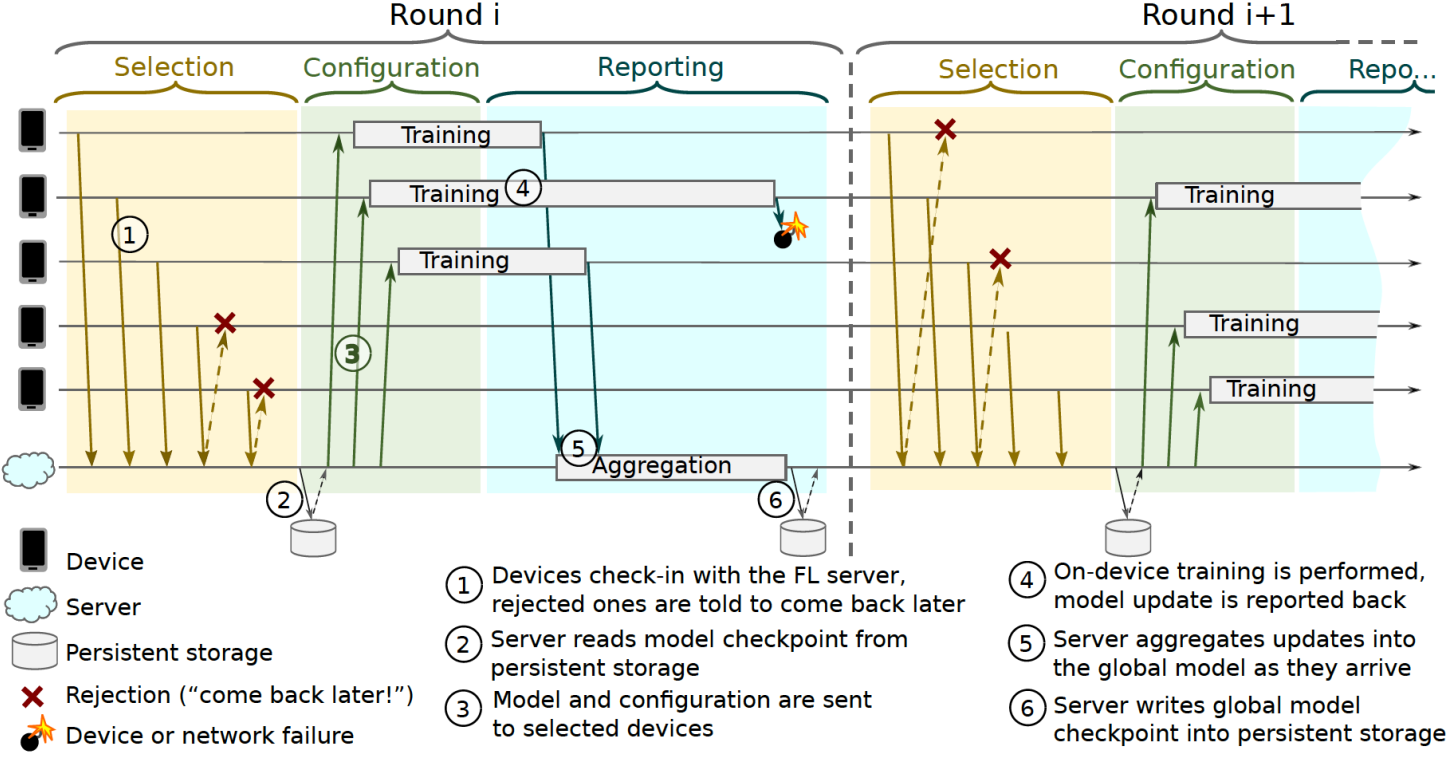
\includegraphics[width=1\textwidth]{Images/fl_protocol.png}
        \decoRule
        \caption[FL protocol]{FL protocol with stragglers, client disconnections and client selection: \href{https://ieeexplore.ieee.org/document/9060868}{URL}.}
        \label{fig:FL protocol}
\end{figure}

\subsection{Communication cost reduction}
To achieve a satisfactory model in FL, multiple rounds of training and communication between the server and the clients are required. Communication can be a big bottleneck if the ANN being trained is massive and has millions of parameters, or if the clients are under slow connections. As a result, a series of techniques for improving communication efficiency have been developed, which can be classified into three groups: increasing computation, decreasing communication size, and decreasing communication frequency.

\subsubsection{Edge and End Computation}
Increasing parallelism by selecting more clients each global epoch is an obvious technique to increase computation in edge devices. In general, client-wise parallelism is desirable, but it provides diminishing returns as the number of participating clients increases. Furthermore, if all of the connected clients are participating, this strategy is no longer applicable. Finally, there is the risk of rapidly exhausting the available datasets.

The most typical technique to increase computation is to have clients perform more local model updates per global epoch. This can be achieved in two ways, more local epochs, i.e. more passes through the local dataset, or smaller batch size, i.e. more updates per pass through the local dataset. In traditional DL, such techniques tends to produce negative effects like overfitting. On the other hand, FL algorithms, due to their model averaging, produce regularization effects equivalent to dropout, ultimately increasing the accuracy of the model under training.

While these techniques are effective, having too many local updates between communication rounds can have a negative impact. To begin with, local models may diverge too much from each other, especially when under non-IID data distribution, significantly decreasing the convergent rate of the global model. As a result, additional training is required, defeating the aim of these techniques.

Another concern is that the likelihood of stragglers occurring is considerably increased due to client heterogeneity. Clients with fewer resources will take disproportionately longer to complete the additional computations, widening the gap between them and the faster ones. Since simulations are most often used when developing FL algorithms, researchers frequently overlook this issue.

\subsubsection{Model Compression}
These techniques, which are extensively employed in DL, attempt to decrease the amount of the communicated updates. The weights of the model under training make up the majority of the updates; applying transformations like sparification, quantization, and subsambling to them can reduce the size of the updates. In general, they are classified into two types: structured updates, which attempt to select what information is sent, and sketched updates, which attempt to compress the communicated information.

Structured updates require that updates adhere to a set, reduced format. This is possible in multiple ways, like putting a predermined per-client mask on the model after training to sparsify it. Another method is to instruct a client to train and communicate only specific layers or pieces of them. A more complex alternative is for the server to apply dropout to the global model in order to create a submodel, which the clients train, and the server maps back to the global model during aggregation. In general, these methods try to shift the responsibility of compression to the server, with the aim to make it more predictable and correct its error.

Sketched updates refer to techniques that encode the update in one side and decode in the other. One such method is probabilistic quantization \cite{probabilistic_quantization}, in which the update matrices are vectorized and quantized for each scalar. Another option is to use a random mask like in a structure update, with the difference that it is randomly generated by the client and communicated to the server together with the encoded local model.

All these methods can be lossy and introduce error as a result of information loss. This error can be characterized as noise, which in most cases has a mean value of zero due to the nature of the compression algorithms commonly used. As such, the averaging of the FL algorithms can reduce it or even eliminate it from the accumulation of the local updates. For this to be true in practice, a large number of clients must be participating, which that is not always achievable. Moreover, as there is only one global model at any given time, any error in server-to-client communication cannot be reduced.

\subsubsection{Importance-based Updating}
By sending only what seems important, importance-based updating aims to reduce the volume of communication. Based on the observation that most parameters in an ANN are close to zero or hardly vary \cite{observation_parameters}, this can be done in a fine-grained manner by sending to the server only a small percentage of the model parameters. It can also be applied in a coarse-grained way by asking clients to review their updates and send them only if they think they would help the overall model. These techniques have demonstrated that, when applied properly, they can occasionally reduce communication while also increasing accuracy and convergence rate. In contrast, they may produce the opposite effects if used excessively.

\subsection{Systems heterogeneity}
The previously discussed systemic characteristics of FL aggravate issues like straggler mitigation and fault tolerance. The slowest participating client has a significant impact on the duration of a global epoch. They can substantially impede training speed, thus removing them from the process is generally considered. Furthermore, if the server waits indefinitely for the client updates and a client disconnects without notifying, the entire system would hang. These issues are especially prevalent in on-edge setting where there is little information or control over the clients' resources.

FL algorithms must be able to handle heterogeneous hardware and resist against random and unpredictable client drops. A frequent option is to disconnect clients who have not responded within a predetermined amount of time. Additionally, using more clients per epoch than necessary and accepting updates from those who respond first can help to eliminate stragglers. While effective, such strategies can induce biases in favour of the datasets of the fastest clients, reducing the overall accuracy of the model.

More sophisticated proposed solutions include intelligent client selection by only accepting clients that report their resources prior participating or tracking statistics on their overall performance. Such methods are not always feasible since they may jeopardize the privacy of the clients. A major portion of FL research employs simulations and avoid these problems, letting these challenges the least explored.

\subsection{Data distribution}
A dataset is independent and identically distributed (iid) if each example in it has the same probability distribution as the others and all are mutually independent. Models' accuracy, convergence rate, and fairness can all be degraded by training on non-iid datasets. Traditional ML avoids these issues by using a single, massive dataset that the designer is allowed to manipulate. On the other hand, FL encompasses a set of smaller datasets that could differ statistically from one another, and the designer may not be in control of or even aware of these differences. Ideally, a global dataset could be established by aggregating all of these small local datasets, however in reality this is impossible because the data cannot be centralized.

\begin{figure}[H]
    \centering
        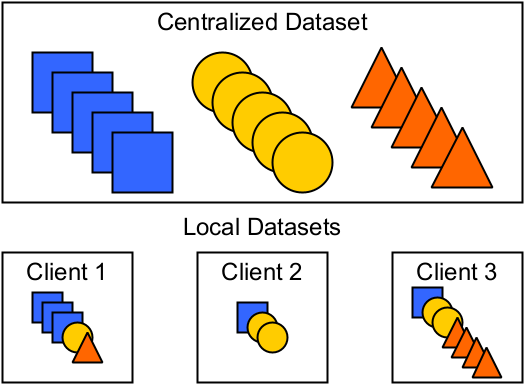
\includegraphics[width=0.6\textwidth]{Images/block_diagrams/data_distribution.png}
        \decoRule
        \caption[Data distribution]{Centralized Dataset vs. Local Datasets. When distributed unevenly among the clients, the same data can behave as non-iid.}
        \label{fig:Data distribution}
\end{figure}

\subsubsection{Non-identical client distributions}
A global dataset used during FL may not be iid for a variety of reasons. First of all, a client's private dataset may locally violate independence, but this can usually be fixed via local shuffling. The statistical variations between the local datasets are more significant.

The distribution of a local dataset \(P_i(x,y)\) can be rewritten as \(P_i(y|x)P(x)\) and \(P_i(x|y)P(y)\), where \(x\) and \(y\) are the input-output pairs. The distributions of at least two clients, I and j, must differ for the data to be non-iid, that is \(P_i \neq P_j\). There are several causes for this, including:

\begin{itemize}
  \item \emph{Feature distribution skew} (covariate shift), \(P_i(x) \neq P_j(x)\):\\
  Even if \(P_i(y|x) = P_j(y|x)\), the marginal distributions \(P(x)\) may differ. This is frequent in the domain of handwriting recognition, where two clients may write the same text in a different writing style.
  
  \item \emph{Label distribution skew} (prior probability shift), \(P_i(y) \neq P_j(y)\):\\
  Even if \(P_i(x|y) = P_j(x|y)\), the marginal distributions \(P(y)\) may differ. This is common when clients are bound to specific locations. Clients from different areas may use different terms and phrases depending on their local accent and lingo.
  
  \item \emph{Same label, different features (concept drift)}, \(P_i(x|y) \neq P_j(x|y)\):\\
  Even if \(P_i(y) = P_j(y)\), the marginal distributions \(P(x|y)\) may differ. The same label \(y\) can have different meaning for different users based on their culture and standard of leaving. Images of clothes, for example, can vary greatly according on location.
  
  \item \emph{Same features, different label (concept shift):}, \(P_i(y|x) \neq P_j(y|x)\):\\
  Even if \(P_i(x) = P_j(x)\), the marginal distributions \(P(y|x)\) may differ. This is very common with labels that reflect sentiment. As an example, clients living in cold climates may describe the same weather phenomena differently than clients lining in warm or temperate climates.
  
  \item \emph{Quantity skew}:\\
  Clients can generate and save different amounts of data. This is dependent on a variety of factors, including available data storage, local data retention laws, and the habits of their users.
  
  \item \emph{Violations of independence}:\\
  Throughout training, the distribution may change at any time. Clients may connect or disconnect, or their local datasets may be exhausted. Furthermore, if clients are available at specific times of day due to solstice, a strong regional bias is imposed. Finally, because the clients own their own datasets, they can modify them at any time during training.
  
  \item \emph{Dataset shift}:\\
  The FL participants might not be indicative of the end users. For instance, clients with inferior devices may be underrepresented as a result of any eligibility criteria used during client selection.
\end{itemize}

A real-world FL dataset may have any combination of these effects. Due to the difficulties of generating such datasets and examining algorithms built on them, most research tends to concentrate on one or two of them. Depending on the Fl scenario under training, different distribution skew effects may aplly and different mitigation strategies may be required.

\subsubsection{Dealing with non-iid distributions}
Existing algorithms can be modified, either by altering their parameters and hyperparameters or by sophisticating features like client selection. While adjusting other parameters, reducing batch size and increasing local epochs can be increase model accuracy, but excessive use may hurt convergence rate and lengthen training time. Metalearning approaches could be used to discover an ideal equilibrium.

It has been demonstrated that system heterogeneity and data heterogeneity interplay. By discarding straggles, unique and useful data could be wasted, degrading the model's fairness and accuracy. Stragglers can partially work, by personalizing parameters or reparameterizing on the fly, according to their resources. In this way, their local datasets can be exploited without slowing down the overall process.

Another approach is for the server to request data distribution statistics from the clients. With this information, the server can select those that will result in a balanced distribution. In addition, the server may be able to share some relevant publicly available data with the clients in order to rebalance their datasets. If no such data are available, willing clients may, if practical, provide their datasets to aid in the overall training process. These techniques can alleviate non-iid distribution problems, but they require additional communication and bandwidth. Additionally, they have the potential to compromise privacy, which would undermine one of FL's main goals.

Similarly, frameworks for multitask learning may be employed. Clients can train their local personalized models concurrently with the global model and share knowledge between them. Such techniques may not always be available as they demand greater processing and memory resources from the clients.

\subsection{Privacy and Security}
One of FL's key goals is to protect participants' privacy by simply requesting them to share model parameters and not any of their personal information. Additionally, FL wants to improve the model's fairness and accuracy by incorporating personal data. However, if any FL participant is malicious, these goals could be defeated. Model updates obtained from them can be used to reconstruct data, and poisoning attacks can corrupt the model.

\subsection{Types of Attacks} % D

\begin{itemize}
  \item Data poisoning attacks\\
  In order to lower the accuracy of the model and add biases, these attacks introduce tainted data that violate the dataset's integrity. Model skew attacks \cite{Model_skewing_attacks} and feedback weaponization\cite{feedback_weaponization} fall within this group. The goal of model skew attacks is to decrease the model's accuracy by obfuscating or distorting the boundaries between the classifiers. Feedback weaponization, on the other hand, tricks the model into misclassifying certain labels to introduce biases against them.
  
  \item Adversarial attacks \footnote{Also called model poisoning.}\\
  Adversarial attacks \cite{adversarial_attack} involve specially crafted data that have designed to be consistently misclassified by the model. They can be subdivided to non-targeted and targeted. Non-targeted attacks try to evade being correctly classification during inference, any incorrect result is acceptable. Targeted attacks aim to incorporate backdoors into the model, that means manipulate the network to give specific erroneous inference for certain inputs.
  
  \item Inferring Attacks\\
  Attacks of this kind aim to gain information about the participants and their data, and can be classified into two categories. The first one is tracing attacks, which aim to detect whether a client is actively participating into training. The second one reconstruction attacks, which aim to recreate examples used in training, or features of them.
  
  Such attack can perpetrated using model extraction algortihms and Generative Adversarial Networks \cite{GAN_attack} (GANs). GANs is a ML technique where two competing ANNs are trained, a generator network and a discriminator network. The generator tries to create fake data while the discriminator tries to discern real data from the fake by analyzing the output of the discriminator. After some training, the generator can create data that closely resembles the real ones using the statistics learned by the classifier.
  
  A GAN attack seeks to infer as much useful information as possible about elements in a target class that are not under its possession. The GAN tries to mimic samples of that class, mislabels them and feeds them to the ANN under federated training. The rest of the participants must then work harder to discriminate between the target class and the mislabeled class, resulting in additional knowledge about the target class in the global model. This process is repeated until convergence, and the GAN has enough information to reliably reconstruct samples from the target class that approximate the original examples. 
  
  This attack can be generalized to any number of classes and users, as well as any type of collaborative learning. If the server or another entity with access to the victim's communications is the malicious actor,it can be made more efficient by using the victim's local updates rather than the global model.
\end{itemize}

\begin{figure}[H]
    \centering
        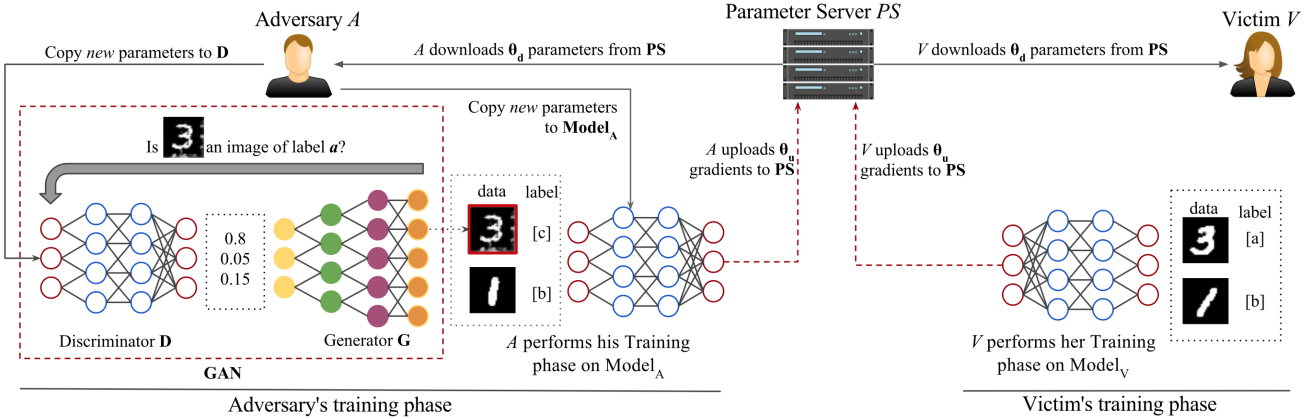
\includegraphics[width=1\textwidth]{Images/topologies/gan_fl.png}
        \decoRule
        \caption[GAN attack]{GAN attack. The adversary mimics images of class \emph{a}, labels them as class \emph{c} and uses them to train the collaborative model. To distinguish between these two classes, the model will require more information from the victim. The adversary does not need to have any true samples.: \href{https://arxiv.org/abs/1702.07464}{URL}.}
        \label{fig:GAN attack}
\end{figure}

\subsubsection{Countermeasures}
FL algorithms are somewhat resistant to the aforementioned attacks due to the regularization effect of averaging local models. Data poisoning and adversarial attacks require a sizable portion of the dataset to be tainted in order to succeed. Additionally, inferring attacks demand that the malicious actor go through numerous training epochs. In an IoT environment since most clients, if they are even chosen, will only participate once. Even when several malicious clients collude, the is a very small probability of achieving their goals.

Such scale is quite challenging to achieve in an environment closer to the datacenter, making it much more vulnerable. Furthermore, clients might seek stronger privacy guarantees as the server might not always trustworthy. For these reasons, further measures for protecting privacy and security are necessary.

An additional level of security can be provided with minimal adjustments to the FL protocol, by scanning the clients' updates for unusual patterns. Repeated updates with outlandish values could be a sign that a client is attempting to corrupt the model. Furthermore, the updates of clients that try to inject backdoors frequently resemble one another, which is rare, especially in a non-iid dataset. Such methods can improve the security of the model, but require plain-text access to the local updates, which is not always available due to privacy enhancements based on cryptography.

Clients might request further privacy protections, particularly if they don't trust the server or the connection between them. Secure Multi-Party Computation (MPC) \cite{MPC}, a subfield of cryptography, can be utilized to accomplish that. MPC simulate a trustworthy third party between two or more collaborating parties. Its homomorphic encryption techniques, which allow mathematical operations to be performed directly on cyphertexts and enable the server to aggregate the local models without having access to their plain-text contents, are particularly helpful. As a result, privacy can be ensured, albeit at a high computational cost that comes with cryptographic operations.

The state of the art method to enhance model security and restrict information exposure is differential privacy (DP) \cite{GAN_attack}. The fundamental tenet of DP is that by blurring a model's weights, they can not be associated with the data they were produced with. In FL, clients add random noise\footnote{Usually Gaussian.},with a mean value zero, to their local updates prior sharing them with the server. In addition of concealing the clients, this technique hinders dackdoor injections to the model, as the malicious clients need to send a precise set of parameters to achieve their goals.


\begin{figure}[H]
    \centering
        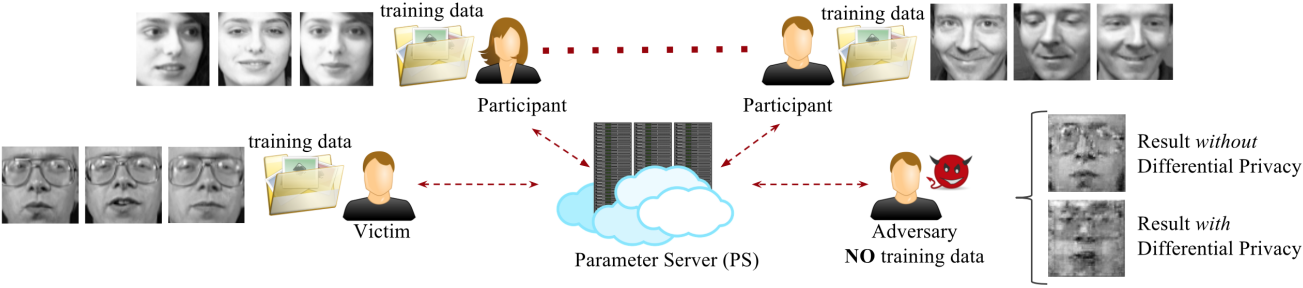
\includegraphics[width=1\textwidth]{Images/topologies/dp_on_gan_attack.png}
        \decoRule
        \caption[GAN attack under Differential Privacy]{Effect of Differential Privacy on a GAN attack.: \href{https://arxiv.org/abs/1702.07464}{URL}.}
        \label{fig:GAN attack under Differential Privacy}
\end{figure}

Theoretically, under DP transformation, the accuracy of the model and its convergence rate won't be impacted as the noise should vanish during aggregation. In practice, several samples are necessary to generate a distribution with a mean value close to zero, thus FL must be scaled appropriately. Finally, as attacks get more sophisticated, these countermeasures might not be effective and combinations of them or new ones are required.

%types
% \subsection{Categorization?} % C12:5 +B88
%     horizontal - vertical - transfer learning?
%     \subsubsection{Architectures for a federated learning system}
\chapter{Related Work}
\label{Chapter-Related-Work}

% Todo: Edit to your liking
\section{Training Datasets}
Common datasets and FL datasets from TF.
\section{FedAvg}
\section{CE-FedAvg}
\section{Evolution of FL}
Fig 5 from A review of applications in federated learning

\section{quantization?}

\section{The FPGA Perspective}
\section{Thesis Approach}

\chapter{FL architecture \& design} %spasimo se fl architecture
\label{Chapter-FL-architecture-design}

%%%%%%%%%%%%%%%%%%%%%%%%%%%%%%%%%%%%%%%%%%%%%%%%%%%%% Software %%%%%%%%%%%%%%%%%%%%%%%%%%%%%%%%%%%%%%%%%%%%%%%%%%%%% 
\section{Software}
\subsection{Tensorflow \& Keras}
TensorFlow \cite{tensorflow2015-whitepaper} is an interface for expressing ML algorithms and an implementation for executing such algorithms. It offers a complete, flexible ecosystem of tools, libraries and community resources that that facilitates the development and deployment of ML powered applications. Its main advantage is the ability to use high-level APIs like Keras with eager execution, enabling immediate model iteration and easy debugging. 

Tesnorflow \& Keras were used in all experiments during modelization. It is chosen due to its simple, flexible architecture, which turns new ideas into code quickly. In addition, due to the existence of TensorFlow Federated (TFF) \cite{tff} framework, there are many compatible theoretical resources and tutorials. TFF is simulating FL to facilitate research and experimentation with FL algorithms, thus it is incompatible with this work which aims to implement real-world FL with hardware accelerators.

\subsection{Python/C API} \label{Python/C API}
As the goal is to integrate FL with FPGA accelerators, the majority of the codebase is developed in C++. This include all the networking, communication, model aggregation and any required model transformations. TensorFlow on Python is utilized for model evaluation and, throughout the modelization phase, for training. To connect these two components, the Python interpreter is embedded to the core program using the Python/C API \cite{Python/C_API, embedding_python}.

With the TensorFlow C API \cite{TF_C_API}, TensorFlow could be used directly in C++, however several capabilities, like the Neural Network library, are not supported. Furthermore, quickly rotating among ANN architectures, training techniques, etc. is quite usual in FL development. With the C API that becomes tedious and slow, since it is geared more toward uniformity and simplicity than convenience, and C++ needs to be recompiled after every change. Due to these factors, integrating the Python interpreter and using TensorFlow in Python is considered as a more appropriate solution.

\subsection{POSIX sockets}
POSIX sockets \cite{POSIX_socket} is an application programming interface (API) for Internet and Unix domain sockets, used for inter-process communication (IPC). A socket is an abstract representation for the local endpoint of a network communication path. According to the Unix philosophy, the POSIX sockets API defines it as a file descriptor that offers a standard interface for input and output to data streams.

The 4.2 Berkeley Software Distribution \cite{bsd} Unix operating system, which was introduced in 1983, is where the API originates from. POSIX sockets transitioned mostly unchanged from a de facto standard to a POSIX specification component. They are commonly referred to as "Berkeley sockets" or "BSD sockets" to acknowledge the Berkeley Software Distribution, where they were first implemented.
 
In FL, entities possess their own private data. This is best implemented through processes with private data space that communicate using sockets. Therefore, the POSIX socket API implementation provided by the LINUX operating system is used for all inter-entity communication. 

POSIX sockets can be configured for blocking or non-blocking operation. In blocking operation, the program halts until the entire message is sent or received. In contrast, during non-blocking operation they only retrieve or send data that is immediately available. Thus, the program does not stall on straggler connections and many deadlock situations are avoided, but there is no guarantees that the messages will be send or received in one piece, especially when said messages are large \footnote{This is due to limited sized socket buffers set up by the operating systems.}.

%%%%%%%%%%%%%%%%%%%%%%%%%%%%%%%%%%%%%%%%%%%%%%%%%%%%% Data Preparation %%%%%%%%%%%%%%%%%%%%%%%%%%%%%%%%%%%%%%%%%%%%%%%%%%%%% 
\section{Data Preparation}
\subsection{Normalization}
Dataset normalization \cite{dataset_norm}, as part of data preparation, is a standard practice in ML. Normalization transforms the features of a dataset to a common scale, without distorting discrepancies in the ranges of values or losing information. This technique prevents large scaled characteristics to dominate during training. Furthermore, many algorithms, such as ReLU non-linearities, exhibit better performance when fed with data of floating-point format.

In this work, the Fashion-MNIST dataset provided by TensorFlow Datasets \cite{TFDS} collection is utilized. It is consisted of gray-scale images, where each pixel is represented by an integer in the range \([0,255]\). They are normalized to floating-point format in the range \([0,1]\) with the script \texttt{prepare\_dataset.py}. Furthermore, to avoid repeating this procedure for every experiment, the processed dataset is saved on disk.

\subsection{Distribution}
In FL, each client is meant to have their own unique, individualized dataset. Given that the provided Fashion-MNIST dataset is a single, concentrated collection, it must be distributed among the clients in order for federated training to be possible. Two approaches of partitioning the data among the clients are explored:

\subsubsection{IID}
The data are randomly partitioned in equally sized shards, one for every client. For example, if there are 10 clients, each will receive a shard containing 6000 examples. Although this distribution is not IID in the strictest sense\footnote{Due the shards being mutually exclusive, knowing that an example belongs to one of them indicates that it does not exist in others shards. Thus, knowledge about the other local datasets can be inferred and independence is violated.}, it is closer to a real-world scenario and many issues, such as class underrepresentation, can be easily avoided.

\subsubsection{non-IID}
Although statistical challenges are not the focus of this study, some testing with non-IID data has been done for sake of completeness. The dataset is broken up into shards, each of which includes examples from only one label. Each client receives two shards of different labels. If there are 10 clients, for instance, twenty shards will be produced, and each client will receive 3000 examples from two labels for a total of 6000 examples. Despite such a pathological non-IID distribution being atypical of a real-world scenario, it will assist investigate how severely the algorithms fail on extremely non-IID data.

\subsection{Pipeline}
The input pipeline that feeds the training data to the models is constructed using the \texttt{tf.data} API provided by TensorFlow. More specifically, before training begins, each client optimizes the use of its dataset by transforming it through caching, shuffling, batching, prefetching, and repeating. Additionally, this process is parameterized for flexibility and enable experimentation with different local dataset and batch sizes.

%%%%%%%%%%%%%%%%%%%%%%%%%%%%%%%%%%%%%%%%%%%%%%%%%%%%% Embedding Python Interpreter %%%%%%%%%%%%%%%%%%%%%%%%%%%%%%%%%%%%%%%%%%%%%%%%%%%%%
\section{Embedding the Python Interpreter}
As mentioned in section \ref{Python/C API}, the Python Interpreter is embedded on top of the C++ codebase. To make this integration as seamless as possible from both sides, an integration layer that operates as a wrapper for the C/Python API, has been developed. The C++ codebase can call Python code with simple function calls, while the Python code can access data from the C++ space like it would access data from its own space.

To achieve this, A number of steps need to be completed. First of all, a strait-forward abstract class is defined, which specifies a train and an evaluate function, as well as an input and an output model. The C++ codebase is interfacing with an implementation of this class. Its tasks include initializing the Python interpreter, loading the appropriate Python module, passing the necessary data and creating C++ function wrappers for the Python function.

Moving data from one side to the other can be trickier than it first appears. Using the appropriate API calls, such as \texttt{PyModule\_AddIntConstant}, simple constants and macros can be passed by copy to the Python module in a strait-forward manner. This approach fails when dealing with large amounts of data, such as the model parameters. Instead, by constructing NumPy array metadata over them and copying them, they can be passed by reference. In this manner, both ends observe the same memory space and there is no significant data copy.

After exposing the parameters to the Python code, one more step is necessary to enable the TesnorFlow library to be able to use them. In order to assign the received parameters to the model under training, they must be first transformed into TesnorFlow tensors with dimensions and shapes that match its layers. Likewise, to extract parameters from a model and expose them to the C++ codebase, its layers must be concated in a NumPy array.


\begin{figure}[H]
    \centering
        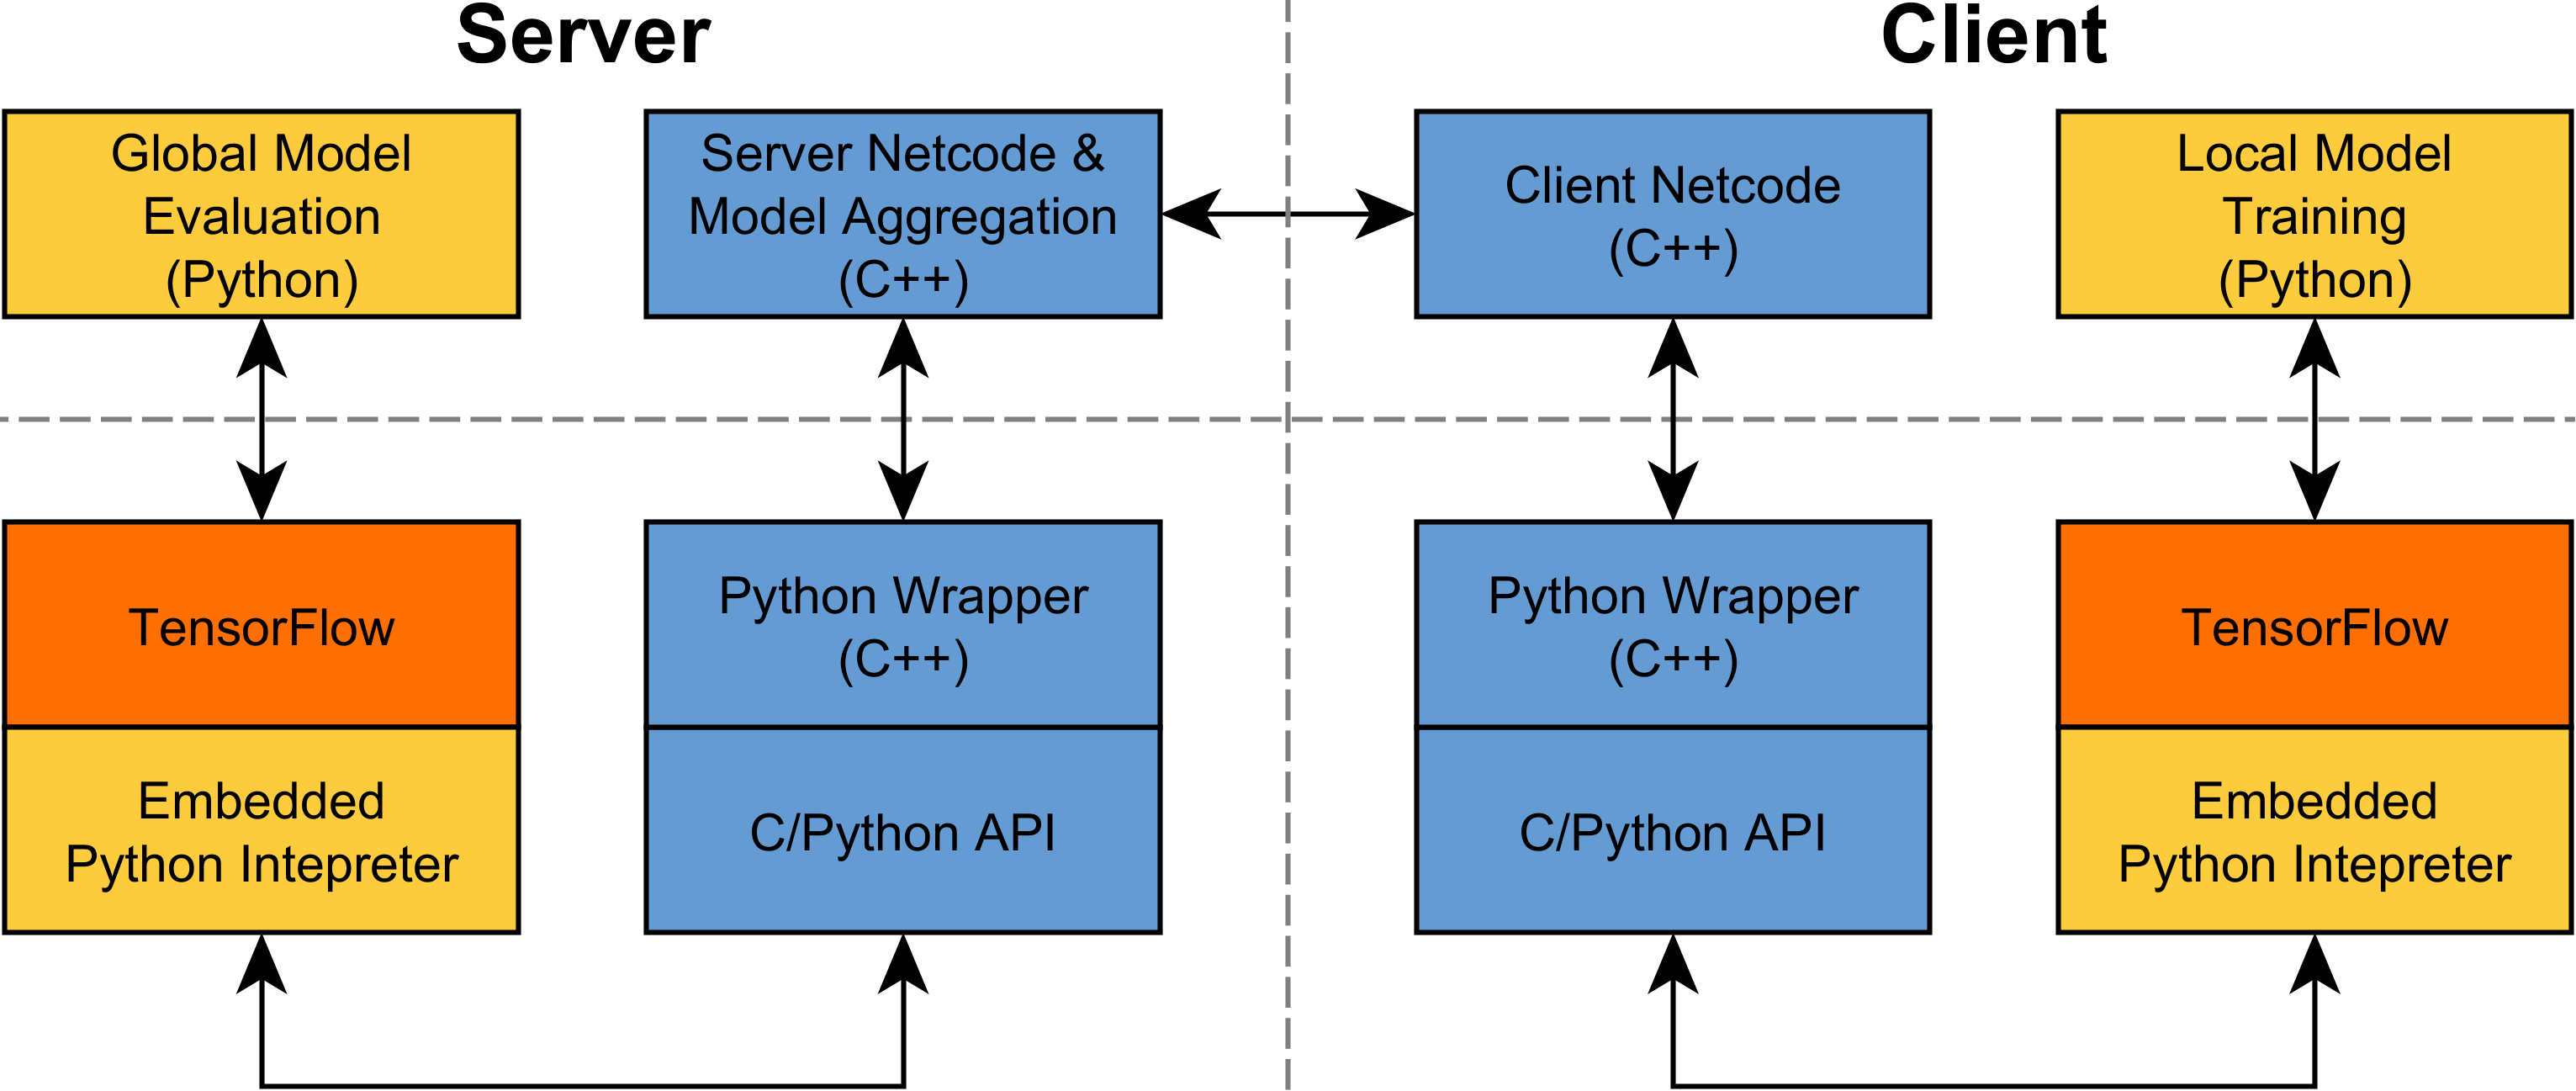
\includegraphics[width=1\textwidth]{Images/block_diagrams/model_lifecycle.png}
        \decoRule
        \caption[C++/Python Integration]{Overview of the C++/Python Integration. The FL protocol implementation components are represented in the top half, while the required libraries, APIs, and wrappers are shown in the bottom half.}
        \label{fig:model_lifecycle}
\end{figure}

%%%%%%%%%%%%%%%%%%%%%%%%%%%%%%%%%%%%%%%%%%%%%%%%%%%%% implementation %%%%%%%%%%%%%%%%%%%%%%%%%%%%%%%%%%%%%%%%%%%%%%%%%%%%% 
\section{FL Architecture}\label{sec:FL_architecture}
The architecture aims to offer a generalized FL loop that enables the implementation of various FL algorithms. To achieve this, it is designed to be flexible and modular, with each FL operation, such as client selection and aggregation, having its own specialized function. Additionally, all relevant training parameters and hyper-parameters, such as local epochs or participating clients per epoch, are compiled in the \texttt{definitions.hpp} file. Since the entire codebase accesses them from there, testing and experimentation are streamlined and less prone to mistakes.

In FL, multiple entities are present, the orchestrating server and the clients training the global model. As the aim of this work is to implement FL with clients operating on separate devices, it is essential that each entity is a distinct process with its own private data-space. That data-space contains its private training or testing dataset, as well as its local or global models. All required communication is facilitated through POSIX sockets.

\begin{figure}[H]
    \centering
        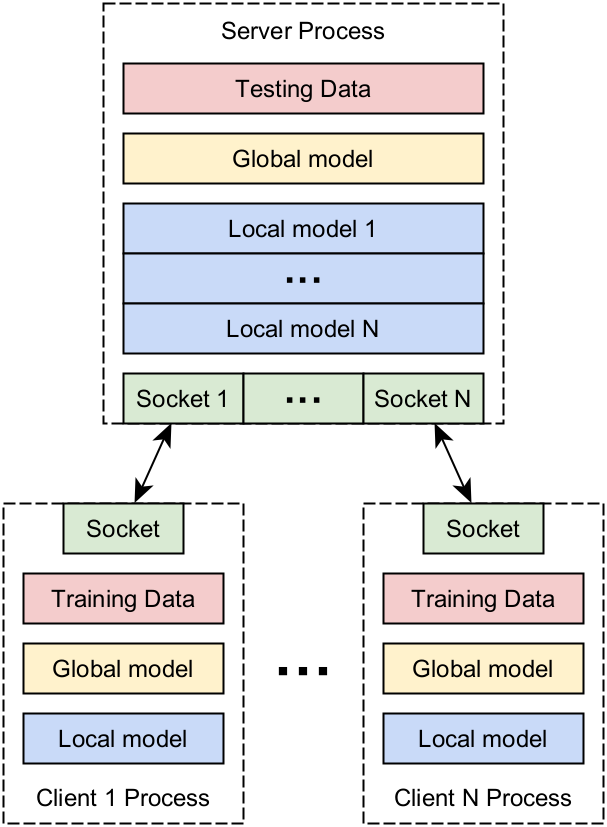
\includegraphics[width=0.5\textwidth]{Images/block_diagrams/memory_layout.png}
        \decoRule
        \caption[Process \& Memory layout]{Process and memory layout of the FL architecture. Each client holds their private data, the global model and the models they produced. Meanwhile, the server holds the testing dataset, the global model and the most recent local model it received. All communication goes through dedicated sockets.}
        \label{fig:process_mem_layout}
\end{figure}

\subsection{Server}
\subsubsection{Overview}
The server generally adheres to the event-driven server paradigm. The process, while sleeping, listens for events such as new connections or messages from the clients, and reacts according to their context. This is very similar to FL in that the server receives local models, aggregates them, and then, after accumulating a sufficient number of them, creates a new global model and announces it to the clients. All these actions are triggered by client updates.

The server process is the focal point of FL and is responsible for several tasks, which can be distinguished between algorithmic, systemic and auxiliary. Algorithmic tasks are the components of the FL algorithm, such as model aggregation. Systemic tasks are necessary operations to implement the FL algorithm, such as connecting sockets. In addition, some tasks that are not required to implement the algorithm are included in order to enhance its utility and ease development.

\subsubsection{Operation}
The server's first action is to load a pre-trained model, if one exists. While not a prerequisite to facilitate FL, this is done to enable transfer learning and experimenting with retraining a model under different settings. 

After that, the server completes a series of initializations. First of all, a listening socket is set-up in non-blocking operation, and the event-driven structure is established. Furthermore, the Python environment, where the global models are evaluated, is embedded and initialized. Finally, any structures or variables required by the FL algorithm are initialized.

After the initializations, the server enters a waiting state. To achieve this the \texttt{poll(2)} system call, which puts the process to sleep until an event occurs, is used. Four types of events may happen:
\begin{itemize}[leftmargin=*]
    \item The listening socket encounters a new connection, meaning a new client requests to join in the federated training. The socket is cloned, the clone establish the connection with the client, and any necessary data structures are created.
    \item A connected socket encounters an error, such as an sudden disconnection. Unreliable clients are expected to continue being unreliable, thus the most prudent course of action is discarding them.
    \item A connected socket receives new data. As a message can consist of millions of weights, it may be received across multiple events and a collection mechanism is needed to fully retrieve it. To achieve this, it is necessary to track the size of the received data per client and ensure that there is always adequate memory available to store a message from each connected client. If the message is complete and valid, its local model is aggregated to next global model, and the related client is considered as non-working.
    \item A connected socket can send new data. This indicates that a socket designated to send the global model to its connected client, is available to do so. As mentioned before, the messages can be quite large, thus multiple events may be required to fully send them. To achieve this, tracking of the amount of transmitted data per connection is necessary. When a message is fully send, the related client is considered as working. Furthermore, as there no more data to send, the \texttt{POLLOUT} flag of the socket is disabled.
\end{itemize}

Following any event, the server determines whether a new epoch should begin. It takes in consideration how many local models were successfully received this epoch, how many clients are connected, and how many clients are still working. If the current epoch requires further work, the process returns to the waiting state and sleeps until a new event occurs.

If the contrary is true, the new global model is created by dividing the aggregated local models by the number of received local models during the current epoch. This new model is evaluated, and then shared with clients that where randomly selected using the Durstenfeld-Fisher-Yates shuffle algorithm \cite{Durstenfeld_Fisher_Yates_paper, Fisher_Yates_shuffle_wiki}. The only action needed to share the model with a client is enabling the \texttt{POLLOUT} flag of the corresponding socket; the event loop will handle sending the message.

The event loop's final step is to determine whether any further training is required. If the target accuracy is achieved or a predetermined number of GEs have been completed, the server shows any relevant statistics, stores the final global model to disk, and shuts down.

% \subsubsection{Memory layout}

\subsection{Client}
\subsubsection{Overview}
During an epoch, a participating client receives a global model, goes through a few local training rounds, and then sends the updated local model back to the server. Training cannot begin until the global model is fully received. Furthermore, after sending the local model, nothing further needs to be done until a new global model is received.

As a result, the client is controlled by its communication with the server, and a master-slave relationship is formed between them. To effectively implement this, client-side communication is blocking, meaning a client can not take any action until it has fully received or send its messages.

\subsubsection{Operation}
At startup, the client creates a socket and connects to the server. Additionally, it embeds and initializes the Python environment that is used for training.  Following these initializations, the process moves into its main loop.

The main loop contains three major operation. First, it receives the global model shared by the server. Then, it is trained with the local private data, creating a new local model. Finally, any required transformations, such as quantization and compression, are applied to the new model, which is then send to the server. This process is repeated until the server informs that there will be no more training with that client.

% \subsubsection{Memory layout}
\begin{figure}[H]
    \centering
        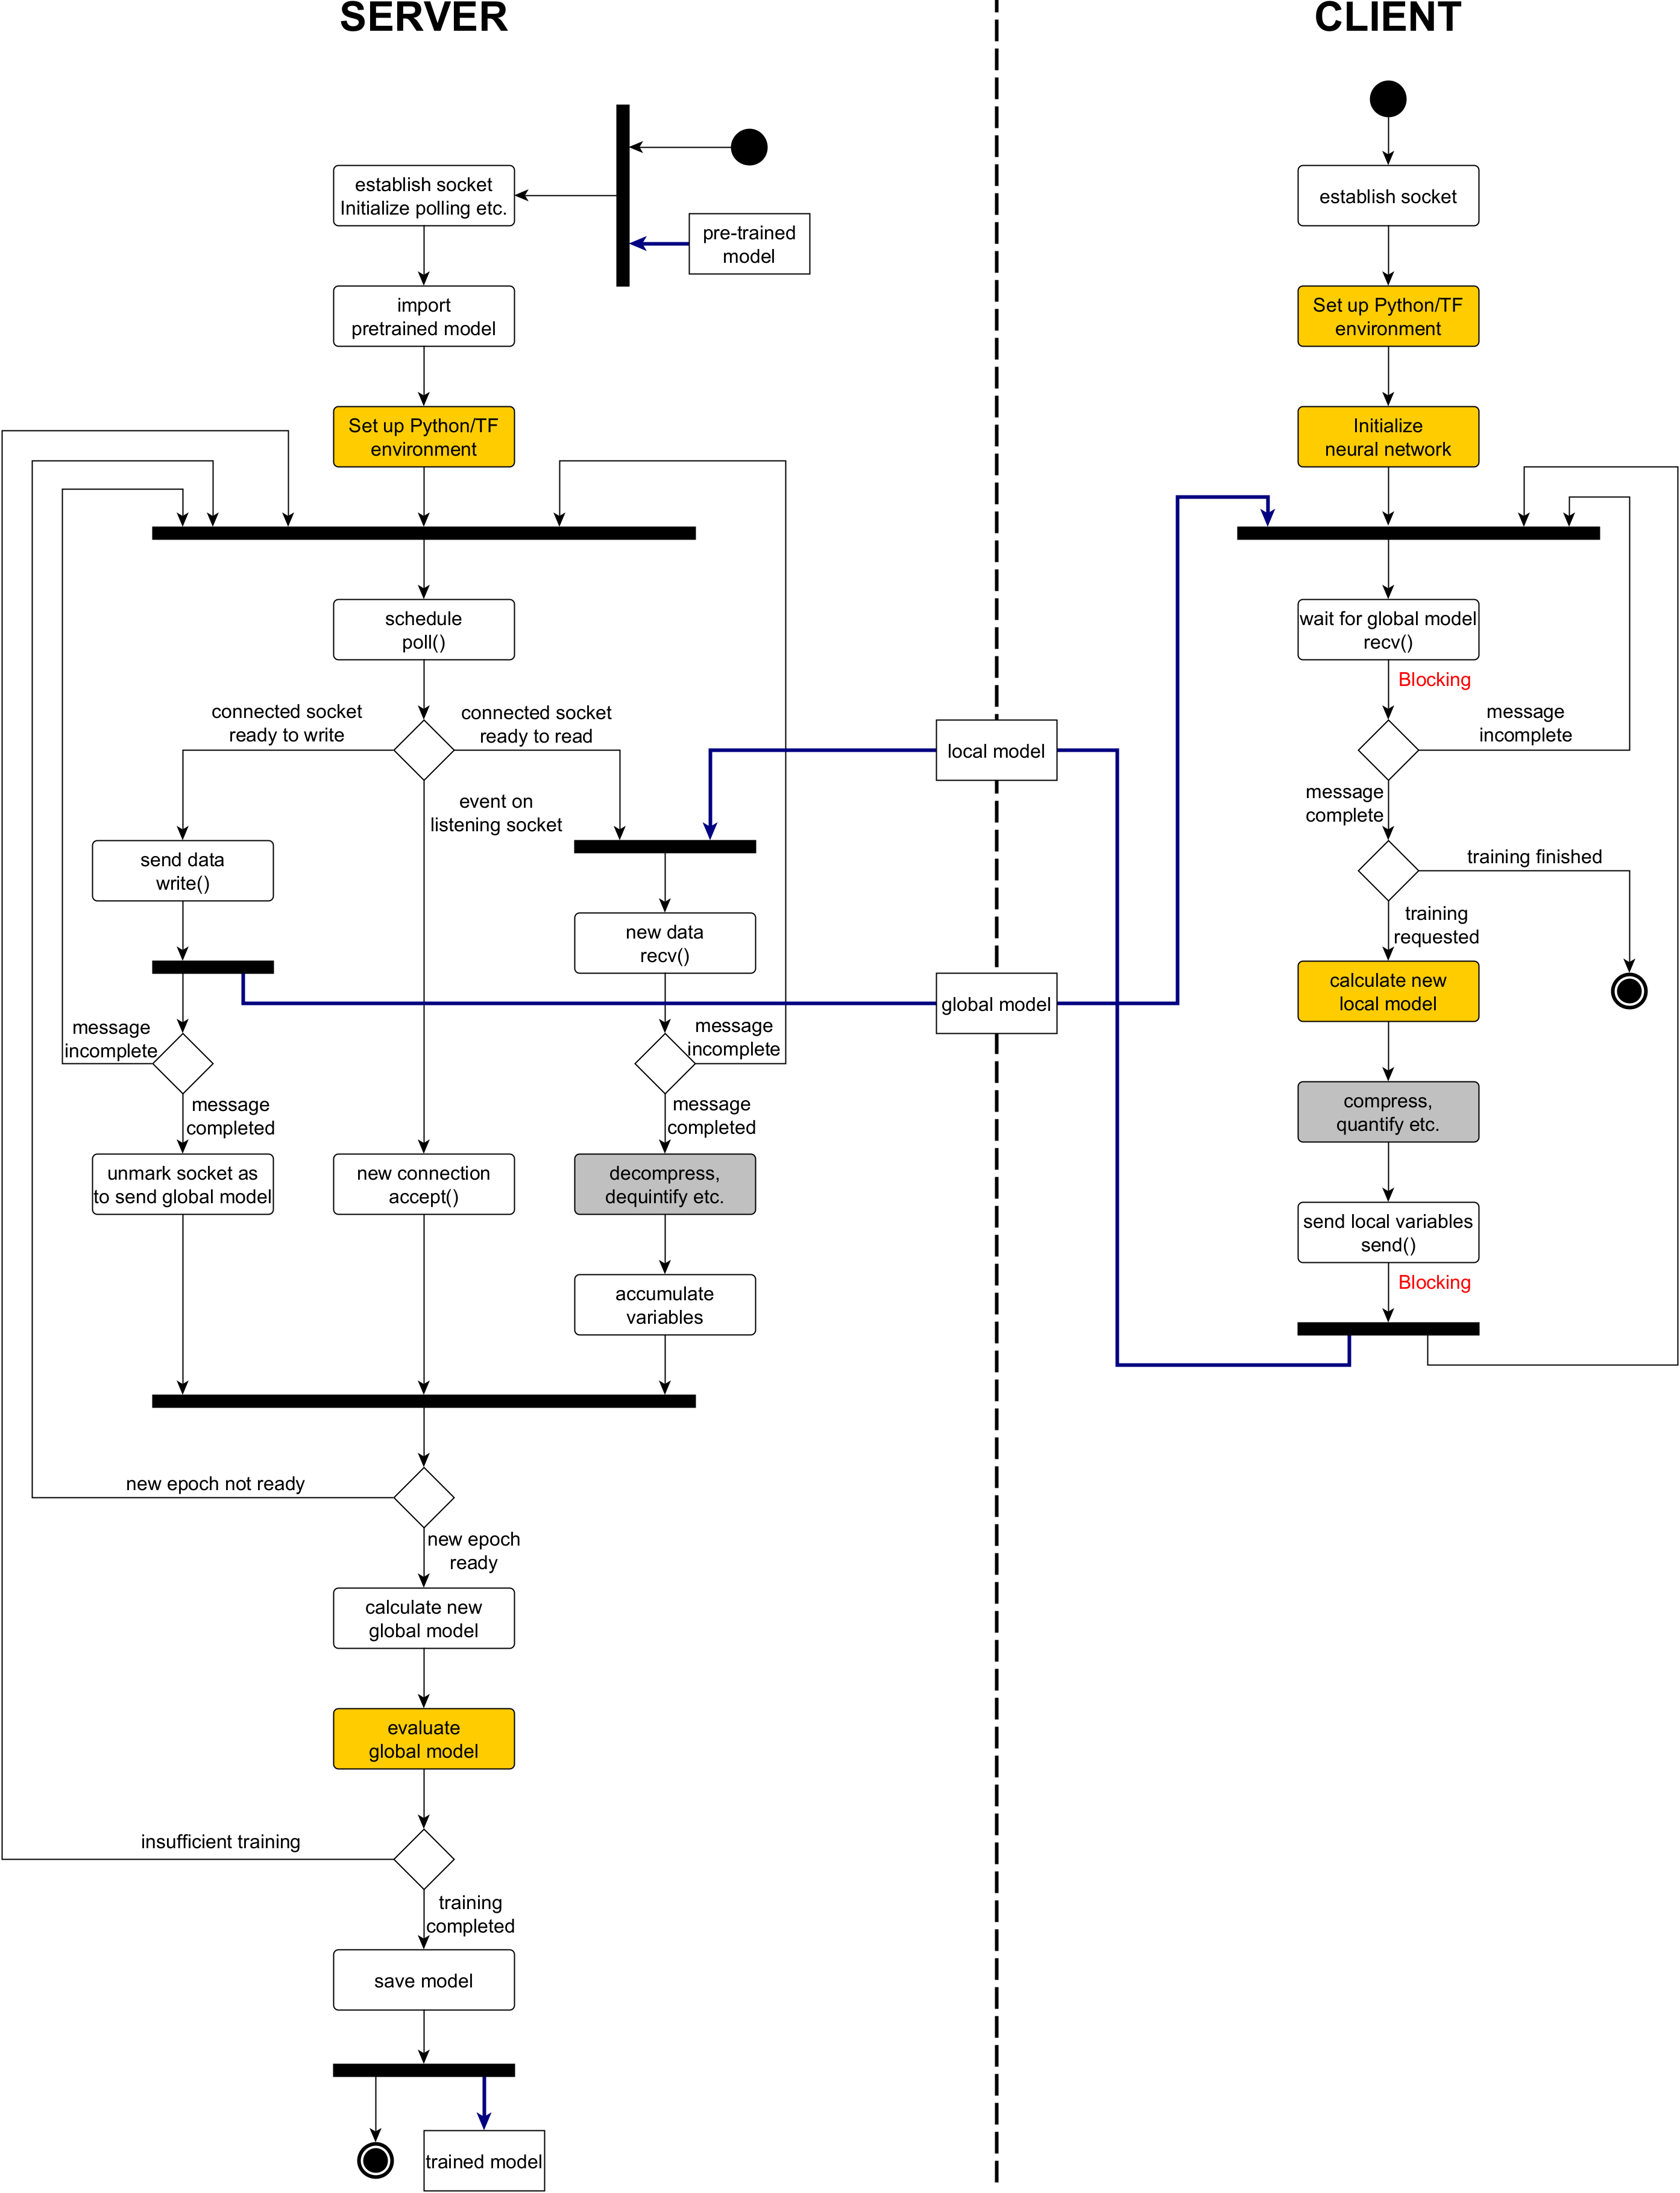
\includegraphics[ width=\textwidth, height=\textheight, keepaspectratio]{Images/block_diagrams/top.png}
        \decoRule
        \caption[Server - Client Activity Diagram]{Server - Client Activity Diagram: Yellow states are modelled with TensorFlow, while grey states are not essential for FL. Blue arrows represent data movements. Error conditions and states are not displayed.}
        \label{fig:server_client_activity_diagram}
\end{figure}
% \subsection{Life cycle of a model?} figure 4.1

\subsection{Communication Scheme}
As stated in section \ref{sec:FL_architecture}, the server and the clients are separate processes that communicate over sockets. A concrete, predefined communication system is needed to accomplish this in a reliable manner. The server holds the barest amount of information on the clients, just what is necessary to stay in connection and communicate, to adhere to the cross-device FL setting.
As such, the server can not address clients directly and messages must be generic. Furthermore, each message must be independent from the rest and self sufficient. As a result, messages sent by the server to clients must be general and self-sufficient.

Algorithmic solutions can reduce communication, but communication must be kept to a minimum in systemic level too. The messages, to be as compact as possible, only include their model and a few bytes of metadata required by the FL algorithm. Furthermore, they are C-aligned arrays, which means there are no delimiters between their values, or hidden metadata from predefined protocols of higher abstraction, such as Protobuf.

Minimizing communication frequency is another strategy used for cutting down on communication time. Any message send by the server that contains the global model, can be interpreted as an request to train it. Furthermore, if a client sends its local model, it can be presumed that it completed its task. As a result, each epoch only these two messages are required, and any synchronization or confirmation messages are unnecessary. With this approach, it is necessary for every party to interpret the messages in a same predefined way.

\begin{table}[H]
    \center
    \begin{tabular}{ | c | }
        \hline
        Server to client message\\
        \hline\hline
        flags\\
        \hline
        GE\\
        \hline
        global model variables\\
        ...\\
        \hline
        \multicolumn{1}{ c }{ } \\
    \end{tabular}
    \quad
    \begin{tabular}{ | c | }
        \hline
        Client to server message\\
        \hline\hline
        GE\\
        \hline
        local loss\\
        \hline
        local accuracy\\
        \hline
        model variables / deltas\\
        ...\\
        \hline
    \end{tabular}
    \caption[Communication Scheme]{The format of the communication between the server and clients.}
    \label{table:FL messages structure}
\end{table}

The format of the messages is shown in Table \ref{table:FL messages structure}. The flags field is intended to communicate particular instructions to clients, such as the message is the final one and no more communication will be accepted or that the client should initialize the model. The GE field is used to discard stragglers, as the server can quickly reject any messages from an earlier GE. The local loss and accuracy fields are used to facilitate complex algorithms, such as ignoring local models with poor accuracy or higher loss than the prior GE. The global and local model parameters are the last part of the format and make up the bulk of the messages.

\subsection{Model Library}
Most ML models, if not all of them, are meant to be trainable in a federated environment. To demonstrate the accuracy of the developed FL environment, a library of ten typical models has been created. As the training problem is image recognition, the majority of the models are CNNs. However, models of different architectures, such as deep and residual ANNs, are also included.

\begin{enumerate}

    \item The simplest model in the library is a DNN architecture. It consists of three fully connected ReLU activated layers with 128, 1024 and 128 neurons respectively, followed by a Softmax layer. In total, it contains 365,066 weights for an approximate size of 1.46 MBytes.
    
    \item The first CNN model follows the original LeNet-5 architecture. It has two convolutional layers of 6 and 16 \(5\times5\) kernels, each one accompanied by an average pooling layer with \(2\times2\) pool size. They are followed by two fully connected layers of 120 and 84 neurons, and a Softmax layer. All layers, except the final one, are activated with the hyperbolic tangent function. In total, it contains 61,706 weights for an approximate size of 0.25 MBytes.
    
    \item For the following experiments, the model most used is a CNN architecture consisting of two convolutional ReLU activated layers of 32 and 64 \(3\times3\) kernels, each accompanied by a max pooling layer with \(2\times2\) pool size. They are followed a 128-neuron fully connected ReLU activated layer, and a Softmax layer. It contains 421,642 weights for an approximate size of 1.69 MBytes. This architecture is compact enough to enable rapid experimentation and testing while being sufficiently sophisticated to provide an acceptable level of accuracy and necessitate several training epochs.
    
    \item The CNN used in the original FL work \cite{FL-original-paper} is also included in the model library. Its architecture is fairly similar with the previous one, but with larger \(5\times5\) kernels, and a fully connected layer of 512 neurons. In total, it contains 1,663,370 weights for an approximate size of 6.65 MBytes.
    
    \item The next model included in the library aims to evaluate the FL environment with more sophisticated layers and combinations between them. It employs six convolutional layers, applies batch normalization on their outputs, and uses max pooling every two convolutions. There are 803,240 weights in it, giving it an approximate size of 3.2 MBytes.
    
    \item To test the FL environment with extremely large models, the AlexNet architecture have been implemented. The model consists of 46,764,746 weights for a message size of 187 MBytes. As a result, it is unfeasible to train it repeatedly, as the FL operation needs, with the current available resources. Instead, it was trained for a single epoch with a few training data and conservative hyperparameters, just to demonstrate that the FL environment has no model size constraints.

    \item For similar reasons the OverFeat-AlexNet architecture is included. This model is the largest one in the library, with 56,906,954 weights and a total size of 227 MBytes. The same constrains apllies.
    
    \item The inception module detailed in section \ref{Inception Module} is the foundation for two of the included models. The first one comprises of two such modules of different sizes and a Softmax layer. It has a total of 4,275,914 parameters and is about 17.1 MBytes in size.
    
    \item The second inception architecture includes a module sandwiched between two convolutional layers, and max pools the outputs of all three. The output of the module is also subjected to the dropout transformation. Furthermore, they are followed by two fully connected layers and then a Softmax layer. In total, there are 277,082 weights for a size of 1.1 MBytes.
    
    \item The final model is based on the residual architecture. It is consisted of two convolutional layers and a Softmax layers. The input of the network feeds the convolutional layers, but it also skips them and is directly connected to the Softmax layer. Furthermore, the dropout transformation is applied to the input of the Softmax layer. It has 539,466 parameters and is about 2.16 MBytes in size.
\end{enumerate}

\chapter{Robustness Analysis}
\label{Chapter-Robustness-Analysis}

A number of experiments, each concentrating on a different component of the FL algorithm, have been conducted to demonstrate the robustness of the developed FL environment. Additionally, the tests begin with straightforward cases and progress to more complicated ones by building on their findings. The training problem is image recognition on the Fashion-MNIST dataset. % why the experiments, from simple cases to more complex ones, problem 

As the main goal of these experiments is to prove the algorithmic soundness of the FL environment, they were carried out on a single machine. As a result, the participating processes are competing for computing resources, and communication takes place on the operating system's loopback. Thus, it is impossible to draw any meaningful real-time inferences from these experiments; instead the communication frequency is used as a benchmark value. % what looking into and why.

\section{Distributed SGD with IID data}
The first experiment focuses on the most straitforward case, distributed SGD with IID data. The training dataset is split equally between the participating clients. The third model in the collection is used, and for simplicity's sake, the Adam optimizer with default parameters is employed. 

\begin{table}[H]
    \center
    \begin{tabular}{ | c | c | }
        \hline
        \multicolumn{2}{ | c | }{ parameters } \\
        \hline\hline
        participating clients & 4 \\
        \hline
        local epochs & 1 \\
        \hline
        steps per epoch & 3 \\
        \hline
        batch size & 10 \\
        \hline
    \end{tabular}
    \caption[Experiment 1 Parameters]{Parameters of the first experiment.}
    \label{table:Experiment 1 parameters}
\end{table}

Using the aforementioned parameters, each client consumes 30 examples per GE. Considering that all four clients participate in each GE, 500 GEs are necessary to exhaust all training data.

The FL trained model is compared to a centrally trained one with same parameters. To do this properly, a common scale is required. As such, the number of times the training dataset is repeated is used.

\begin{figure}[H]
    \center
    \begin{tikzpicture}
    \begin{axis}
        [
            xmin = 0,
            xmax = 21,
            xlabel = Dataset Repetitions,
            xtick = { 1 , 3 ,..., 20 },
            ylabel = Test Accuracy,
            legend pos = south east,
            thick,
            scale = 1.25,
            every node/.style = {transform shape},
            scaled x ticks = false
        ]
        \addplot table [y=FL, x=P]{data/experiment1.dat};
        \addplot +[restrict x to domain=1:15] table [y=LL, x=P]{data/experiment1.dat};
        \addlegendentry{FL training}
        \addlegendentry{Centralized training}
    \end{axis}
\end{tikzpicture}
    \caption[Experiment 1 results]{Experiment 1 results}
    \label{fig:Experiment 1 results}
\end{figure}

The aforementioned findings demonstrate that training the model via FL yields the same accuracy as training it centrally, albeit at a slower rate. This is understandable given that the model in the first case is updated every 150 examples, whereas in the second case it is updated every 10 examples.

Another observation is the re-balancing effect of the FL algorithm. In centralized training, due to overfitting, the accuracy of the model degrades after peaking. This is not true when trained under the federated setting, as overfitted parameters are regularized when averaging multiple local models.

\section{Distributed SGD with non-IID data}
In this experiment, the third model is trained with distributed SGD and a pathological non-IID dataset. It is interesting to see how the batch size affects the performance of Distributed SGD, given that it is notorious for being unable to handle non-IID datasets. Thus, the test was repeated with three distinct combinations of parameters.

\begin{table}[H]
    \center
    \begin{tabular}{ | c | c | c | c | }
        \hline
        case & 1 & 2 & 3\\
        \hline\hline
        participating clients & 5 & 5 & 5 \\
        \hline
        local epochs & 1 & 1 & 1 \\
        \hline
        steps per epoch & 1 & 1 & 1 \\
        \hline
        batch size & 1 & 2 & 4 \\
        \hline
    \end{tabular}
    \caption[Experiment 2 Parameters]{Parameters of the second experiment.}
    \label{table:Experiment 2 parameters}
\end{table}

The dataset is split between 5 clients, with each one getting all the examples of two labels. The first client holds all the examples with labels 0 or 1, the second client holds all the examples with labels 2 or 3 etc. As clients holds no knowledge on the other classes, self-training the model can only achieve a maximum accuracy of 20\%. Therefore, it is required to either centralize the dataset or use a decentralized training method.

\begin{figure}[H]
    \center
    \begin{tikzpicture}
    \begin{axis}
        [
            xmin = 0,
            xmax = 21,
            xlabel = Dataset Repetitions,
            xtick = { 1 , 3 ,..., 20 },
            ylabel = Test Accuracy,
            legend pos = south east,
            thick,
               % scale = 1.25,
            every node/.style = {transform shape},
            scaled x ticks = false
        ]
        \addplot table [ x=P , y=b1 ]{data/experiment2.dat};
        \addplot table [ x=P , y=b2 ]{data/experiment2.dat};
        \addplot table [ x=P , y=b4 ]{data/experiment2.dat};
        
        % \addplot [ very thin , blue ] 
        %     gnuplot [raw gnuplot] {
        %          f(x) = a * x^3 + b * x^2 + c * x + d;
        %          a = 0.0001;
        %          b = 0.0001;
        %          c = 0.1;
        %          d = 80;
        %          fit f(x) 'data/experiment2.dat' using 1:2 via a,b,c,d; 
        %          plot [x=1:20] f(x);
        %     };
        % \addplot [ very thin , red ] 
        %     gnuplot [raw gnuplot] {
        %          f(x) = a * x^3 + b * x^2 + c * x + d;
        %          a = 0.0001;
        %          b = 0.0001;
        %          c = 0.1;
        %          d = 80;
        %          fit f(x) 'data/experiment2.dat' using 1:3 via a,b,c,d; 
        %          plot [x=1:20] f(x);
        %     };
        % \addplot [ very thin , olive ] 
        %     gnuplot [raw gnuplot] {
        %          f(x) = a * x^3 + b * x^2 + c * x + d;
        %          a = 0.0001;
        %          b = 0.0001;
        %          c = 0.1;
        %          d = 80;
        %          fit f(x) 'data/experiment2.dat' using 1:4 via a,b,c,d; 
        %          plot [x=1:20] f(x);
        %     };
        
        \addlegendentry{batch size = 1}
        \addlegendentry{batch size = 2}
        \addlegendentry{batch size = 4}
        
    \end{axis}
\end{tikzpicture}
    \caption[Experiment 2 results]{Experiment 2 results}
    \label{fig:Experiment 2 results}
\end{figure}

Distributed SGD appears to struggle with non-IID data. With a batch size of just one example, it achieves accuracy consistent with prior works\cite{FL-original-paper}, but it is unable to converge with bigger batch sizes. This observation is consistent with FL theory, and in order to improve outcomes, additional techniques such as data rebalancing or expanding the client pool are needed.

\section{Client Selection}
In FL, it is frequently preferable to use a portion of the clients in each GE when there are several of them. In this method, data efficiency and model performance are improved since the global model can be updated more times before the training data run out. This experiment aims to test this functionality.

Eight clients are participating in training the Lenet-5 model. Every GE, only three clients are used. The dataset is split into 8 identically sized, mutually exclusive random shards, each of which is given to a client.

\begin{table}[H]
    \center
    \begin{tabular}{ | c | c | }
        \hline
        \multicolumn{2}{|c|}{ parameters } \\
        \hline\hline
         total clients & 8 \\
        \hline
        clients per GE & 3 \\
        \hline
        local epochs & 1 \\
        \hline
        steps per epoch & 2 \\
        \hline
        batch size & 20 \\
        \hline
    \end{tabular}
    \caption[Experiment 3 Parameters]{The parameters of the third experiment.}
    \label{table:Experiment 3 parameters}
\end{table}

Data reshuffling is also incorporated in FL and centralized training. When all of the examples of a dataset have been used, it is resuffled and rebatched. Overfitting is thereby expected to diminish in both scenarios.

\begin{figure}[H]
    \center
    \begin{tikzpicture}
    \begin{axis}
        [
            xmin = 0,
            xmax = 21,
            xlabel = Dataset Repetitions,
            xtick = { 1 , 3 ,..., 20 },
            ylabel = Test Accuracy,
            legend pos = south east,
            thick,
               % scale = 1.25,
            every node/.style = {transform shape},
            scaled x ticks = false
        ]
        \addplot table [ x=session , y=FL_training ]{data/experiment3.dat};
        \addplot table [ x=session , y=local_training ]{data/experiment3.dat};
        
        \addlegendentry{FL training}
        \addlegendentry{Centralized training}
    \end{axis}
\end{tikzpicture}
    \caption[Experiment 3 results]{Experiment 3 results}
    \label{fig:Experiment 3 results}
\end{figure}

In comparison to the first trial, where there was no client selection, FL training produces results that are comparable to those of centralized training more quickly. Furthermore, overfitting is decreased in both scenarios.

\section{Greater data per GE consumption}
The primary objective of this experiment is to assess the impact of increasing the consumption of local data per GE, prior migrating to the Federated Averaging algorithm. Furthermore, the FL environment is tested with a more complex architecture by using the ninth model that contains an inception module and a dropout layer.

The data is distributed randomly to 5 clients, but only 3 of them are used each GE. Two sets of parameters are used, with different number of local updates per GE.
    
\begin{table}[H]
    \center
    \begin{tabular}
        { | l | c | c | c | }
        \hline
        parameters & FL set 1 & FL set 2 & Centralized training\\\hline
        total clients & 5 & 5 & 1\\\hline
        clients per GE & 3 & 3 & 1\\\hline
        steps per GE & 1 & 2 & examples/batch size \\\hline
        batch size & 20  & 20  & 20 \\\hline
        examples per GE & 60  & 120  & all \\\hline
        GEs to use all examples & 1000  & 500  & - \\\hline
    \end{tabular}
    \caption[Experiment 4 parameters]{Experiment 4 parameters}
    \label{table:Experiment 4 parameters}
\end{table}

It is important to note that, compared to the first set of parameters, the second one needs only half as many communication rounds to exhaust the dataset.
    
\begin{figure}[H]
    \center
    \begin{tikzpicture}
    \begin{axis}
        [
            xmin = 0,
            xmax = 21,
            xlabel = Dataset Repetitions,
            xtick = { 1 , 3 ,..., 20 },
            ylabel = Test Accuracy,
            legend pos = south east,
            thick,
               scale = 1.25,
            every node/.style = {transform shape},
            scaled x ticks = false
        ]
        \addplot table [ x=session , y=set1 ]{data/experiment4.dat};
        \addplot table [ x=session , y=set2 ]{data/experiment4.dat};
        \addplot table [ x=session , y=local_training ]{data/experiment4.dat};
        
        \addlegendentry{FL set 1}
        \addlegendentry{FL set 2}
        \addlegendentry{Centralized training}
    \end{axis}
\end{tikzpicture}
    \caption[Experiment 4 results]{Experiment 4 results}
    \label{fig:Experiment 4 results}
\end{figure}

Both FL scenarios reach comparable accuracy with centralized training. Although the second one appears to progress at a slower pace than the first, it only updates the global model half as often and needs half as much communication. This results in double the computation to communication ratio and being a more viable target for parallelization.

\section{Client Fault Tolerance}
In an edge environment, the clients may be unreliable and any algorithm must be resilient to random faults. This experiment aims to simulate such a case. To achieve this, 6 clients are initially participating in training the third model, but around 1/10 into training one of them abruptly disconnects. That means for 90\% of the training, 1/6 of the data are inaccessible.

\begin{table}[H]
    \center
    \begin{tabular}
        { | l | c | c | }
        \hline
        parameters & normal op & faulty op\\\hline
        total clients   & 5 & 6\\\hline
        clients per GE  & 3 & 3\\\hline
        steps per GE    & 1 & 1\\\hline
        batch size      & 20 & 20\\\hline
    \end{tabular}
    \caption[Experiment 5 parameters]{Experiment 5 parameters}
    \label{table:Experiment 5 parameters}
\end{table}
    
\begin{figure}[H]
    \center
    \begin{tikzpicture}
    \begin{axis}
        [
            xmin = 0,
            xmax = 21,
            xlabel = Dataset Repetitions,
            xtick = { 1 , 2 ,..., 20 },
            ylabel = Test Accuracy,
            legend pos = south east,
            thick,
               scale = 1.25,
            every node/.style = {transform shape},
            scaled x ticks = false
        ]
        \addplot table [ x=session , y=normal_operation ]{data/experiment5.dat};
        \addplot table [ x=session , y=faulty_client ]{data/experiment5.dat};
        \addplot[mark=*] coordinates {(2,0.823400020599365)} node[pin=0:{client disconnects}]{} ;
        
        \addlegendentry{Normal operation}
        \addlegendentry{Faulty operation}
        
    \end{axis}
\end{tikzpicture}
    \caption[Experiment 5 results]{Experiment 5 results}
    \label{fig:Experiment 5 results}
\end{figure}

Although the model's final accuracy drops, the effect is manageable as training continues and accuracy is still within acceptable bounds. In a real-world scenario, this issue can be resolved by postponing a portion of the training until after lost data resurfaces or new data becomes available.

\section{Neural Network initialization}

The initialization of an ANN can have a significant impact on the final accuracy, convergence rate, and training time, according to FL theory. It is generally accepted that the best course of action is to use the same initialization for all clients \cite{FL-original-paper}.  This major objective of this experiment is to assess this convention. To further emphasize the consequences of the initialization, the SGD optimizer with a low learning rate is employed.

\begin{table}[H]
    \center
    \makebox[0pt]{
        \begin{tabular}
            { | l | c | c | c | }
            \hline
            parameters & FL seeded init & FL random init & centralized training\\\hline
            total clients & 5 & 5 & 1\\\hline
            clients per GE & 3 & 3 & 1\\\hline
            steps per GE & 5 & 5 & examples/batch \\\hline
            batch size & 20  & 20  & 20 \\\hline
            examples per GE & 300  & 300  & all \\\hline
            GEs to use all examples & 200  & 200  & - \\\hline
        \end{tabular}
    }
    \caption[Experiment 6 parameters]{Experiment 6 parameters}
    \label{table:Experiment 6 parameters}
\end{table}

The third model is used and initialized with the Glorot initializer. The model is trained twice, once initialized with the same seed across all clients, the other using random different seeds.

\begin{figure}[H]
    \center
    \begin{tikzpicture}
    \begin{axis}
        [
            xmin = 0,
            xmax = 41,
            xlabel = Dataset Repetitions,
            xtick = { 1 , 4 ,..., 40 },
            ylabel = Test Accuracy,
            legend pos = south east,
            % scale = 1.25,
            every node/.style = {transform shape},
            scaled x ticks = false
        ]
        \addplot table [ x=session , y=different_init ]{data/experiment6.dat};
        \addplot table [ x=session , y=same_init ]{data/experiment6.dat};
        \addplot +[restrict x to domain=1:20] table [ x=session , y=local_training ]{data/experiment6.dat};
        
        \addlegendentry{FL, seeded initialization}
        \addlegendentry{FL, random initialization}
        \addlegendentry{Local training}
    \end{axis}
\end{tikzpicture}
    \caption[Experiment 6 results]{Experiment 6 results}
    \label{fig:Experiment 6 results}
\end{figure}

The model with a random initialization quickly approaches and settles in a suboptimal local minimum. Both centralized training and FL with seeded initialization surpass its accuracy. This behaviour is consistent with FL theory.

\section{Learning Rate (LR) decay strategies}
Another aspect of FL worth investigating is learning rate (LR) decay strategies. The following three of them are implemented:
\begin{itemize}
    \item Decay the LR every set number of GEs. All clients have the same LR at every moment.
    \item Decay the LR of a client based on the number of participated GEs. If a subset of the clients is used every GE, some clients may have been selected more times than others and as a result they will have a lower LR.
    \item The final strategy is to reduce a client's LR each time its dataset is repeated. This is an extension of the second strategy, where instead of decaying slowly the LR every few rounds, there is a big drop every \( \displaystyle \frac{\sum_{}^{}clients\ data}{\sum_{}^{} clients\ data\ used\ per\ GE} \) rounds of training.
\end{itemize}

\begin{table}[H]
    \center
    \hspace*{-9mm} \makebox[0pt]
    {
        \begin{tabular}
            { | l | c | c | c | c | }
            \hline
            parameters & FL, no decay & FL strategy 1 & FL strategy 2 & FL strategy 3\\\hline
            total clients   &     5 &     5 &     5 &     5\\\hline
            clients per GE  &     3 &     3 &     3 &     3\\\hline
            steps per GE    &     5 &     5 &     5 &     5\\\hline
            batch size      &    20 &    20 &    20 &    20\\\hline
            initial LR      &  1e-2 &  1e-2 &  1e-2 &  1e-2\\\hline
            LR decay        &     - & 0.999 & 0.999 &\( \displaystyle \frac{ 0.999 * \sum clients\ data}{\sum_{}^{} clients\ data\ used\ per\ GE} \)\\\hline
            \makecell{ decay interval\\(x = decay period) } & - & x GEs & \makecell{ x participated\\GEs } &
            \( \displaystyle \frac{ x\ participated\ GEs*\sum clients\ data }{ \sum clients\ data\ used\ per\ GE } \)\\\hline
        \end{tabular}
    }
    \caption[Experiment 7 parameters]{Experiment 7 parameters}
    \label{table:Experiment 7 parameters}
\end{table}

Each strategy is tested three times with different decay periods. The decay period dictates how often the decay applies. E.g. the second strategy with the a decay period of three means that LR decays every three participated rounds. A FL trained model without LR decay is used as a baseline.
\medskip\medskip
\begin{figure}[H]
    \center
    \addtolength{\leftskip} {-2cm}
    \addtolength{\rightskip}{-2cm}
    \begin{tikzpicture}
    \begin{axis}
        [
            xmin = 0,
            xmax = 41,
            ymin = 0.86,
            xlabel style = {align=center},
            xlabel = Dataset Repetitions,
            xtick = { 1 , 4 ,..., 40 },
            ylabel = Test Accuracy,
            legend pos = south east,
            scale = 1,
            no markers
        ]
        \addplot [black] table [ x=session , y=no_decay ]{data/experiment7.dat};
        \addplot [red] table [ x=session , y=s1_dp1 ]{data/experiment7.dat};
        \addplot [blue] table [ x=session , y=s1_dp2 ]{data/experiment7.dat};
        \addplot [green] table [ x=session , y=s1_dp3 ]{data/experiment7.dat};
        
        \addlegendentry{no decay}
        \addlegendentry{ x = 1 }
        \addlegendentry{ x = 2 }
        \addlegendentry{ x = 3 }
    \end{axis}
\end{tikzpicture}%
    \begin{tikzpicture}
    \begin{axis}
        [
            xmin = 0,
            xmax = 41,
            ymin = 0.86,
            xlabel style = {align=center},
            xlabel = Dataset Repetitions,
            xtick = { 1 , 4 ,..., 40 },
            ylabel = Test Accuracy,
            legend pos = south east,
            scale = 1,
            no markers,
        ]
        \addplot [black] table [ x=session , y=no_decay ]{data/experiment7.dat};
        \addplot [red] table [ x=session , y=s2_dp1 ]{data/experiment7.dat};
        \addplot [blue] table [ x=session , y=s2_dp2 ]{data/experiment7.dat};
        \addplot [green] table [ x=session , y=s2_dp3 ]{data/experiment7.dat};
        
        \addlegendentry{no decay}
        \addlegendentry{ x = 1 }
        \addlegendentry{ x = 2 }
        \addlegendentry{ x = 3 }
    \end{axis}
\end{tikzpicture}
    \caption[Experiment 7 results]{Experiment 7 results, strategies 1 and 2.}
\end{figure}%
\begin{figure}[H]\ContinuedFloat
    \center
    \begin{tikzpicture}
    \begin{axis}
        [
            xmin = 0,
            xmax = 41,
            ymin = 0.86,
            xlabel style = {align=center},
            xlabel = Dataset Repetitions,
            xtick = { 1 , 4 ,..., 40 },
            ylabel = Test Accuracy,
            legend pos = south east,
            scale = 1,
            no markers
        ]
        \addplot [black] table [ x=session , y=no_decay ]{data/experiment7.dat};
        \addplot [red] table [ x=session , y=s3_dp1 ]{data/experiment7.dat};
        \addplot [blue] table [ x=session , y=s3_dp2 ]{data/experiment7.dat};
        \addplot [green] table [ x=session , y=s3_dp3 ]{data/experiment7.dat};
        
        \addlegendentry{no decay}
        \addlegendentry{ x = 1 }
        \addlegendentry{ x = 2 }
        \addlegendentry{ x = 3 }
        
    \end{axis}
\end{tikzpicture}
    \caption[Experiment 7 results]{Experiment 7 results, strategy 3.}
    \label{fig:Experiment 7 results}
\end{figure}

All strategies seems to to perform slightly better than the baseline, except the first one with decay period = 1. In that case, the decay is too fast and the LR degenerates in a state that cannot substantially alter the weights of the NN. The last strategy appears to be the most promising, which while outperforming the others is the most straightforward.

\section{Federated Averaging (FedAvg)}
In FedAvg, a client, when participating in a training round, uses all of its data and executes multiple SGD iterations. In the prior experiment, for a client to consume all of its data 200 GEs were necessary; whereas with FedAvg, only one GE (at most) is needed. The main objective of this experiment is to demonstrate the algorithm's compatibility with the developed FL environment.

\begin{table}[H]
    \center
    \begin{tabular}
        { | l | c | }
        \hline
        parameters & FedAvg\\\hline
        total clients   & 5\\\hline
        clients per GE  & 3\\\hline
        local epochs    & 1\\\hline
        steps per epoch & 600\\\hline
        batch size      & 20\\\hline
        initial LR      &  1e-2\\\hline
    \end{tabular}
    \caption[Experiment 8 parameters]{Experiment 8 parameters}
    \label{table:Experiment 8 parameters}
\end{table}

The LR decay needs to be corrected to account for the reduced number of decay events, thus the model is trained multiple times to identify its ideal values. The prior experiment's LR decay is utilized for the first run of training, and each additional training reduces the descent slope by half. The model is also trained without LR decay.
    
\begin{figure}[H]
    \center
    \begin{tikzpicture}
    \begin{axis}
        [
            xmin = 0,
            xmax = 50,
            ymin = 0.8,
            xlabel = GE,
            xtick = { 1 , 5 ,..., 50 },
            ylabel = Test Accuracy,
            legend pos = south east,
            scale = 1.25,
            no markers,
        ]
        \addplot [blue] table [ x=GE , y={lr_decay=0.818649} ]{data/experiment8.dat};
        \addplot [red] table [ x=GE , y={lr_decay=0.9093245} ]{data/experiment8.dat};
        \addplot [green] table [ x=GE , y={lr_decay=0.95466225} ]{data/experiment8.dat};
        \addplot [yellow] table [ x=GE , y={lr_decay=0.977331125} ]{data/experiment8.dat};
        \addplot [black] table [ x=GE , y={no_decay} ]{data/experiment8.dat};
        \addplot[ domain=0:50 , mark=none , black , thin , dotted , samples=2 ] {0.92};
        
        \addlegendentry{LR decay $\approx$ 0.819}
        \addlegendentry{LR decay $\approx$ 0.909}
        \addlegendentry{LR decay $\approx$ 0.955}
        \addlegendentry{LR decay $\approx$ 0.977}
        \addlegendentry{No decay}
    \end{axis}
\end{tikzpicture}
    \caption[Experiment 8 results]{Experiment 8 results}
    \label{fig:Experiment 8 results}
\end{figure}

The maximum accuracy of this model when trained locally is 92\%. This is now regarded as the minimum baseline. In addition of showing maximum accuracy, the GE where that baseline was reached is also presented.

\begin{table}[H]
    \center
    \begin{tabular}
        { | c | c | c | }
        \hline
        LR decay & Max accuracy & 0.92 @GE\\\hline
        0.819 & 0.913 & -\\\hline
        0.909 & 0.9232 & 30\\\hline
        0.955 & 0.9245 & 32\\\hline
        0.977 & 0.9245 & 27\\\hline
        No decay & 0.9224 & 34\\\hline
    \end{tabular}
    \caption[Experiment 8 results]{Experiment 8 results}
    \label{table:Experiment 8 results}
\end{table}

In comparison to the previous experiment, FedAvg requires \(\times\)100-200 less communication and the same computation to reach the target accuracy. However, there is a hidden cost in that less averaging occurs and the rebalancing effect is diminished. This becomes quite clear when training without LR decay, where overfitting is apparent.

Considering the different LR decay values, the more conservative options appear to perform best; decaying the LR too quickly causes the ANN to set in sub-optimal minima.

\section{Client Participation and Increasing parallelism}
This experiment explores the amount of multi-client parallelism that can be exploited and its effect on training. The dataset is split between 10 clients, each one holding 6000 training examples. The third model is trained with different number of participating clients per GE. 
    
\begin{table}[H]
    \center
    \begin{tabular}{ | l | c | c | c | c | }
        \hline
        Test & A & B & C & D\\\hline
        total clients   & 10 & 10 & 10 & 10\\\hline
        clients per GE  & 1 & 3 & 5 & 10\\\hline
        local epochs    & 1 & 1 & 1 & 1\\\hline
        steps per epoch & 300 & 300 & 300 & 300\\\hline
        batch size      & 20 & 20 & 20 & 20\\\hline
        initial LR      & 1e-2 & 1e-2 & 1e-2 & 1e-2\\\hline
        LR decay        & 0.977 & 0.977 & 0.977 & 0.977\\\hline
    \end{tabular}
    \caption[Experiment 9 parameters]{Experiment 9 parameters}
\end{table}

Training with one client per epoch serves as the baseline. The relative reduction in communication is calculated for the other training runs.

\begin{figure}[H]
    \center
    \begin{tikzpicture}[baseline=(current axis.outer east)]
    \begin{axis}
        [
            xmin = 0,
            xmax = 200,
            ymin = 0.8,
            xlabel = GE,
            xtick = { 1 , 20 ,..., 200 },
            ylabel = Test Accuracy,
            legend pos = south east,
            % scale = 1.25,
            no markers,
            thin
        ]
        \addplot [black] table [ x=GE , y={client1} ]{data/experiment9.dat};
        \addplot +[restrict x to domain=1:100] [red] table [ x=GE , y={client3} ]{data/experiment9.dat};
        \addplot +[restrict x to domain=1:100] [green] table [ x=GE , y={client5} ]{data/experiment9.dat};
        \addplot +[restrict x to domain=1:100] [blue] table [ x=GE , y={client10} ]{data/experiment9.dat};
        \addplot [ domain=0:200 , mark=none , black , thin , dotted , samples=2 ] {0.92};
        
        \addlegendentry{1 client per GE}
        \addlegendentry{3 clients per GE}
        \addlegendentry{5 clients per GE}
        \addlegendentry{10 clients per GE}
        
    \end{axis}
\end{tikzpicture}
    \caption[Experiment 9 results]{Experiment 9 results}
    \label{fig:Experiment 9 results}
\end{figure}

\begin{table}[H]
\center
    \begin{tabular}{ | c | c | c | }
        \hline
        client per GE & 0.92 @GE\\\hline
        1 & 159\\\hline
        3 & 61 (2.6$\times$)\\\hline
        5 & 46 (3.4$\times$)\\\hline
        10 & 51 (3.1$\times$)\\\hline
    \end{tabular}
    \caption[Experiment 9 results]{Experiment 9 results, with relative reduction in GEs.}
\end{table}
    
Using more clients per GE substantially lowers the rounds of communication needed to achieve the target accuracy. This is consistent with others works, which show even on simulations of hundreds of clients with a small dataset each, using a bit more than half of the clients in each GE yields the best results. If all the clients are used every GE, especially when under non-IID data, the model may not converge in an acceptable solution.
    
\section{Increasing computation per client}
To further reduce communication, clients can perform more local updates per GE. This may be accomplished by increasing the number of local epochs (LE), reducing the batch size (B), or both. The third model is trained by 5 clients, with 3 of them participating each GE. LR and its decay are amortized to maintain a consistent LR at each GE, regardless of the number of local updates. The goal of this experiment is to identify the behavior of the algorithm across different sets of parameters.

\begin{table}[H]
    \center
    \begin{tabular}{ | c | c c | c c | }
        \hline
        & \multicolumn{2}{|c|}{Local epochs = 1} & \multicolumn{2}{|c|}{Local epochs = 3} \\\hline
        B & updates/GE &  0.92 @GE & updates/GE &  0.92 @GE\\\hline
        600 & 20 & 309 & 60 & -\\
        300 & 40 & 212 & 120 & 67\\
        100 & 120 & 72 & 360 & 36\\
        80 & 150 & 54 & 450 & 25\\
        40 & 300 & 31 & 900 & 13\\
        20 & 600 & 25 & 1800 & 7\\
        10 & 1200 & 18 & 3600 & 15\\\hline
    \end{tabular}
    \caption[Experiment 10 results]{Experiment 10 results}
\end{table}

According to the results of the experimental, increasing local updates directly decreases the required global updates. Unlike most works, this one concentrates on small groups of clients with large local datasets. As a result, increasing the number of local epochs produces inconsistent results due to the introduction of overfitting in the local models. Regarding the batch size, there is no cost in reducing it, providing that it is large enough to completely utilize the client's hardware parallelism. % TODO: break in two parts
\chapter{FPGA Design \& Implementation} 
% architecutr &design & impementation
\label{Chapter-FPGA-Implementation}

\section{Tools Used}
\subsection{Vitis Unified Software Platform}
The Vitis unified software platform\cite{Vitis_unified_software_platform} is a collection of tools, libraries and environments designed to ease the development of accelerated applications tailored for AMD Xilinx FPGA and Versal® ACAP hardware platforms. It includes graphical and command-line compilers, analyzers, and debuggers to build applications, analyze performance bottlenecks, and debug accelerated algorithms, developed in C, C++, or OpenCL APIs. Furthermore, it offers numerous advantages such as effortless application portability, complete simulation of hardware systems, and an open source runtime that handles host-device communication.
\begin{figure}[H]
    \centering
        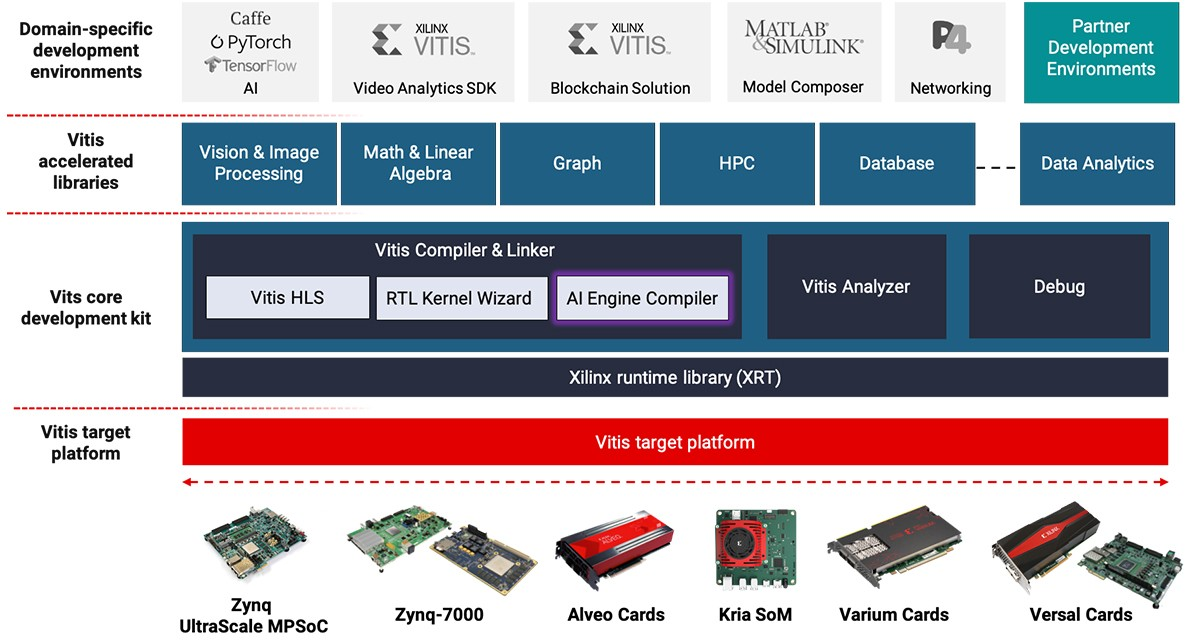
\includegraphics[width=1\textwidth]{Images/Platform/vitis.jpg}
        \decoRule
        \caption[Vitis]{Vitis overview: \href{https://www.xilinx.com/products/design-tools/vitis/vitis-platform.html\#overview}{URL}.}
        \label{fig:Vitis_overview}
\end{figure}

Vitis supports hardware acceleration kernels controlled by PS or x86 kernels. The Vitis application acceleration development flow provides a framework for developing and delivering FPGA-accelerated applications using standard programming languages for both software and hardware components. The kernels can be developed through traditional RTL, C/C++ with Vitis HLS, the Vitis model composer and the AI Engine compiler.
\begin{figure}[H]
    \centering
        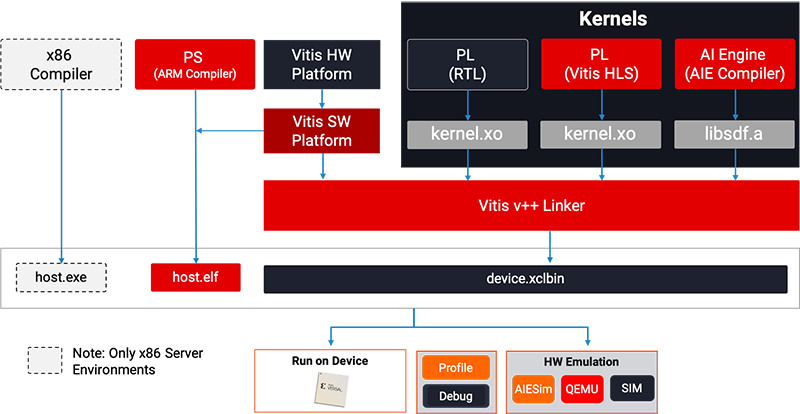
\includegraphics[width=1\textwidth]{Images/Platform/vitis_kernel.png}
        \decoRule
        \caption[Vitis]{Vitis kernel architecture: \href{https://www.xilinx.com/products/design-tools/vitis/vitis-platform.html\#development}{URL}.}
        \label{fig:Vitis_kernel_overview}
\end{figure}

\subsection{Xilinx Runtime library (XRT)}
The Xilinx Runtime library\cite{Xilinx_Runtime_Library} (XRT) facilitates communication between the application code (running on an embedded Arm or x86 host) and the accelerators deployed on the reconfigurable portion of PCIe interface-based AMD Xilinx accelerator cards, MPSoC-based embedded platforms, or ACAPs. It is flexible with modifiable libraries and drivers, enabling different levels of abstractions, from high-level Python bindings to low-level C++ APIs. These APIs are common across all platforms and eliminate the need to implement hardware communication layers from scratch. % what is XRT

A widely used alternative are the OpenCL libraries. TBy abstracting the underlying implementations of numerous APIs, including the XRT, they offer a standard interface for managing heterogeneous devices. As a result, they enable portability across multiple devices from various providers, albeit with increased complexity due to the extra layer of abstraction. As this work is not indented to transition to other devices, the XRT is preferred. % why I chose XRT over OpenCL

\begin{figure}[H]
    \centering
        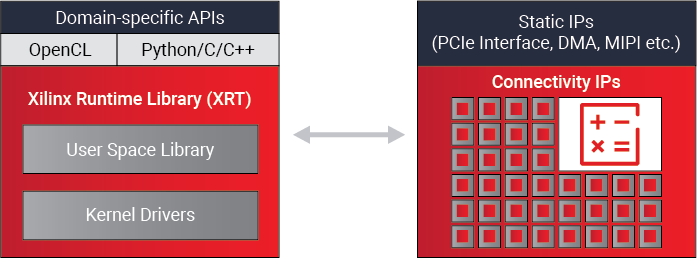
\includegraphics[width=1\textwidth]{Images/Platform/xrt.png}
        \decoRule
        \caption[Xilinx Runtime Library]{Xilinx Runtime Library overview: \href{https://www.xilinx.com/products/design-tools/vitis/xrt.html}{URL}.}
        \label{fig:XRT_overview}
\end{figure}

\subsection{Vitis High Level Synthesis (HLS)}
The Vitis HLS tool can synthesize a C/C++ function into RTL code for implementation in the programmable logic (PL) region of a Xilinx FPGA device. Its kernels can be easily integrated into a design utilizing OpenCL\cite{OpenCL} code. It provides support of complex data types, math functions and AXI4-Stream interfaces for data exchange between IPs in the PL and/or Processing Subsystem (PS).

HLS is an automated design process that takes an abstract behavioral specification of a digital system and generates a register-transfer level structure that implements the given behavior. The designer is working on a high abstraction level, while the tool takes care of mechanical RTL implementation tasks.

\begin{table}[H]
    \center
    \begin{tabular}{ | c | }
        \hline
        Designer's Responsibilities\\
        \hline
        Macro Architecture\\
        Design Intent\\
        Constrains\\
        \hline
        \multicolumn{1}{ c }{ } \\
        \multicolumn{1}{ c }{ } \\
        \multicolumn{1}{ c }{ } \\
        \multicolumn{1}{ c }{ } \\
    \end{tabular}
    \quad
    \begin{tabular}{ | c | }
        \hline
        HLS tool automation\\
        \hline
        FSM Generation\\
        Operation Scheduling\\
        Clock\\
        Register Pipelining\\
        Resource Sharing\\
        Timing\\
        Verification\\
        \hline
    \end{tabular}
    \caption[HLS responsibilities]{Distribution of work during HLS design.}
    \label{HLS responsibilities}
\end{table}

\section{FPGA Platforms}

\subsection{Xilinx Zynq UltraScale+ MPSoC}
The Zynq\textsuperscript{\textregistered} UltraScale+\texttrademark{} MPSoC is a family of Xilinx products that integrates a feature-rich 64-bit quad-core or dual-core Arm® Cortex®-A53 and dual-core Arm Cortex-R5F based processing system (PS) and Xilinx programmable logic (PL) UltraScale architecture in a single device. In addition, on-chip memory, multiport external memory interfaces, and a rich set of peripheral connectivity interfaces are included. \cite{Zynq_UltraScale_overview}

\subsection{ZCU102 Evaluation Board}
The ZCU102 Evaluation Board features a Zynq\textsuperscript{\textregistered} UltraScale+\texttrademark{} MPSoC with a quad-core Arm\textsuperscript{\textregistered} Cortex\textsuperscript{\textregistered}-A53, dual-core Cortex-R5F real-time processors, and a Mali\texttrademark{}-400 MP2 graphics processing unit based on Xilinx's 16nm FinFET+ programmable logic fabric. It supports all major peripherals and interfaces, enabling development for a wide range of applications. Furthermore, its high speed DDR4 memory interfaces, variety of communication interfaces and FMC expansion ports makes it ideal for rapid prototyping. 

\begin{figure}[H]
    \centering
        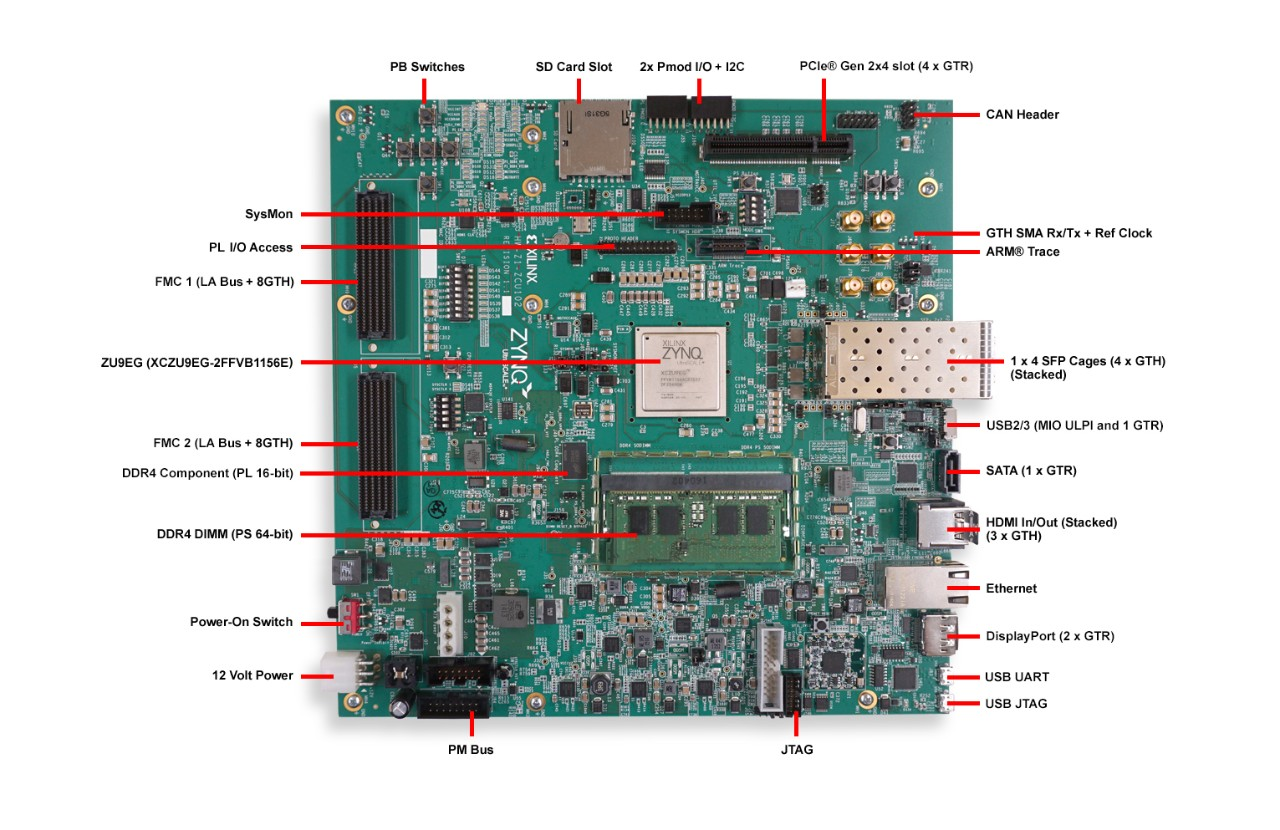
\includegraphics[width=1\textwidth]{Images/Hardware/zcu102.jpg}
        \decoRule
        \caption[ZCU102]{ZCU102 Features: \href{https://www.xilinx.com/products/boards-and-kits/ek-u1-zcu102-g.html\#information}{URL}.}
        \label{fig:ZCU102}
\end{figure}

Given that the thesis is based on an edge application, this platform seems to be an ideal fit for it. During the hardware design phase, the constrains and resource limitation were placed according to the specifications of this board. Nevertheless, transferring the final design to devices of similar families should require minimal effort.

\section{Preparing the CNN for Hardware}
In the preceding phase, TF with Python was utilized to implement all ANNs and training. As the Vitis Kernel Toolchain is aimed to C/C++ code, these implementations can not be synthesized to hardware by the aforementioned tools. As such, a simplified version of the most used CNN, the third in the model library, has been re-implemented with C++.

Migrating from TF to a hardware synthesizable CNN is a fairly challenging task riddled with pitfalls. This implementation is not optimized for hardware, but rather serves as a stepping stone between TF and synthesizable code. Certain practices are adopted to facilitate future transition to hardware targeted code:

\begin{itemize}[leftmargin=*]
    \item Implementation is modular and re-configurable. The code is build around template functions, each of which performs a specified task. Layers can effortlessly added, removed, or altered in size, shape and parameters.
    \item All data, whether input, output or internal, are produced and consumed serially and only once. This behavior is similar to the stream data format, which is widely utilized in hardware design.
    \item All feature maps, input gradients, variable gradients, and updated variables are logged and compared with those generated by the existing TF implementation. This approach not only evaluates functionality, but also produces test benches for future hardware implementation.
\end{itemize}

\begin{figure}[H]
    \centering
        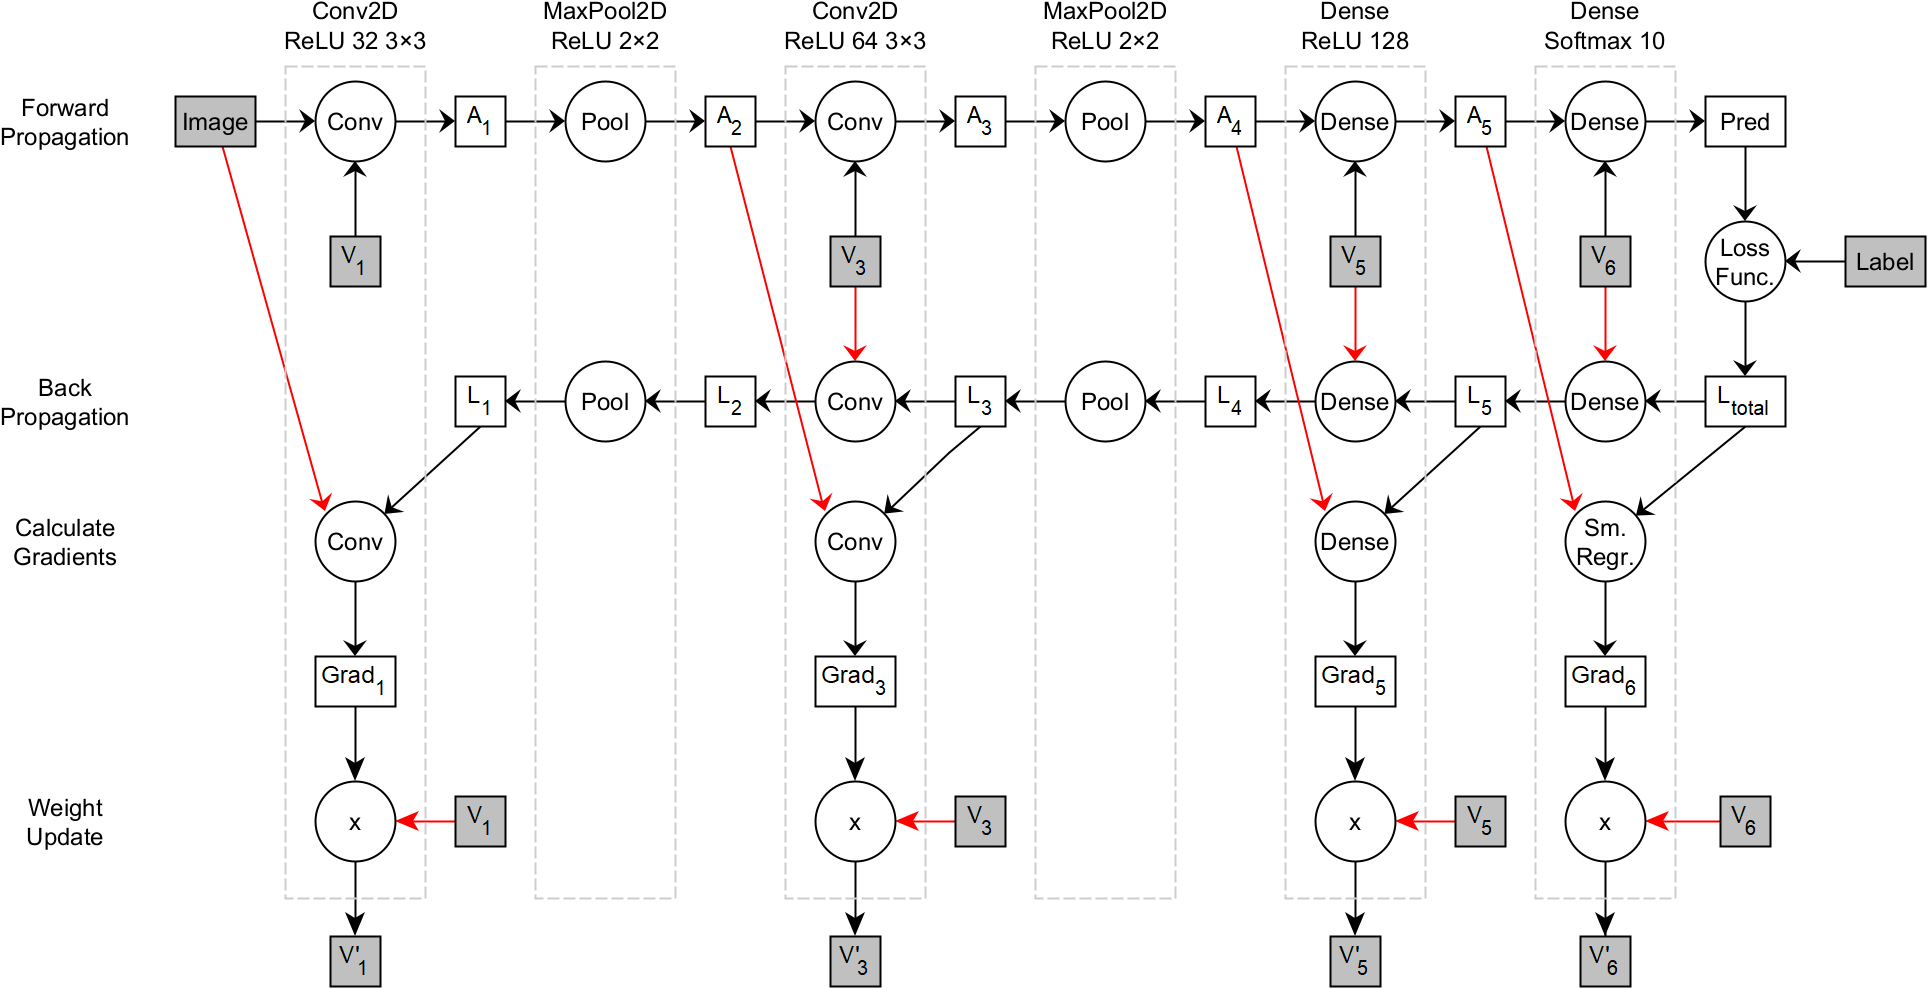
\includegraphics[width=1\textwidth]{Images/block_diagrams/dataflow_cnn_model.png}
        \decoRule
        \caption[CNN dataflow]{Dataflow diagram of the utilized CNN model.}
        \label{fig: CNN dataflow}
\end{figure}

Figure \ref{fig: CNN dataflow} depicts the basic structure of the implementation. Tasks are represented by cycles, whereas data are represented by squares. Inputs, labels, weights and any other data that must to be saved in memory have greyed-out squares. The majority of internal data are consumed immediately after being produced. Some of them, marked by red arrows, skip parts of the chain and must be temporally stored.

\section{Vitis HLS Hardware Implementation}
Even with the aforementioned techniques, adapting the code to be compatible with FPGAs is not a trivial task. To build an efficient implementation, resource usage, data access patterns, and other factors must be taken into account. All parts of the CNN are modified accordingly.

\subsection{2D Convolutional Layers}
Due to their non-serial data access patterns, multi-dimensional filter algorithms frequently conflict with FPGA design; 2-D convolution is no exception. At its core, it carries out some form of data averaging around a pixel, necessitating the access of nearby input values as seen in figure \ref{fig: convolution access pattern}. Additionally, when calculating the adjacent outputs, some inputs are accessed again.

\begin{figure}[H]
    \centering
        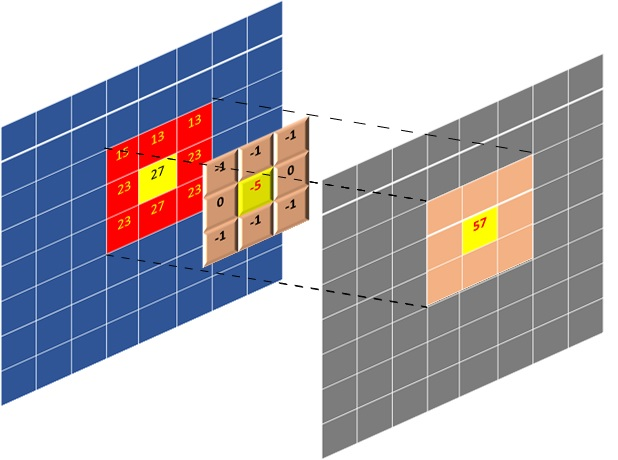
\includegraphics[width=1\textwidth]{Images/diagrams/convolution_access_pattern.jpg}
        \decoRule
        \caption[convolution access pattern]{Convolution access pattern: Input (Blue) pixels are accessed in a non-serial pattern.\href{https://github.com/Xilinx/Vitis-Tutorials/blob/2022.1/Hardware_Acceleration/Design_Tutorials/01-convolution-tutorial/lab1_app_introduction_performance_estimation.md}{URL} }
        \label{fig: convolution access pattern}
\end{figure}

In a CPU-focused implementation this would be a non issue, as data caching and pre-fetching can ensure that the majority of accesses will be cache hits. Implementing this on an FPGA would produce numerous small non-burst accesses on the global memory, resulting in unacceptable performance. Thus, a different approach is required.

A unique data mover, specifically designed for the given algorithm, has been developed to reduce the number of global memory accesses. Its key concept is to construct two-dimensional input windows that are the same size as the filters and then compute the dot product of those. Its main components are buffers that store lines of the input, and a sliding window on top of them.

\begin{figure}[H]
    \centering
        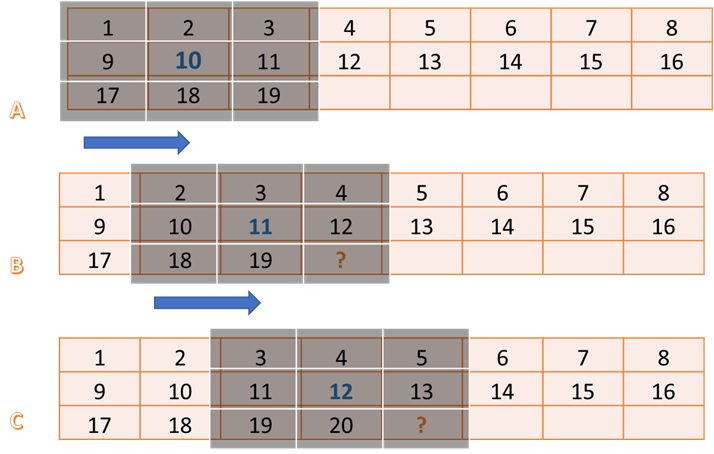
\includegraphics[width=1\textwidth]{Images/diagrams/line_buf_conv.jpg}
        \decoRule
        \caption[Line Buffers, Convolution]{Line Buffers: Sifting a 3x3 window. \href{https://github.com/Xilinx/Vitis-Tutorials/blob/2022.1/Hardware_Acceleration/Design_Tutorials/01-convolution-tutorial/lab2_conv_filter_kernel_design.md}{URL} }
        \label{fig: Line Buffers Convolution}
\end{figure}

Figure \ref{fig: Line Buffers Convolution} illustrates the operation of the line and window buffering scheme. A continuous stream of 3x3 windows is produced by sifting a window buffer over the top of the line buffers. Since the masked elements of the top line are already present in the window, only two line buffers are needed. Furthermore, only one new input pixel is required to produce a window, and thus an output pixel. Finally, zero padding is applied to maintain correct data with edge windows.

To complete the 2D convolution, a processing element is required. In the simplest scenario, a single channel input, the dot products between the windows and the filters are calculated and activated with the ReLU function. If there are additional input channels, the dot products are calculated in respect of each channel, which are aggregated and then activated to produce the feature map of the layer. This is done to allow computing of multiple channels in parallel, while using a data streaming paradigm.

Two output streams are produced, one float and one bool. The first one consists of the activations and is connected to the next layer. The second one indicates whether or not the kernels have activated the ReLU function. As only activated neurons convey their error backwards, this is necessary information for the back-propagation.

\begin{figure}[H]
    \centering
        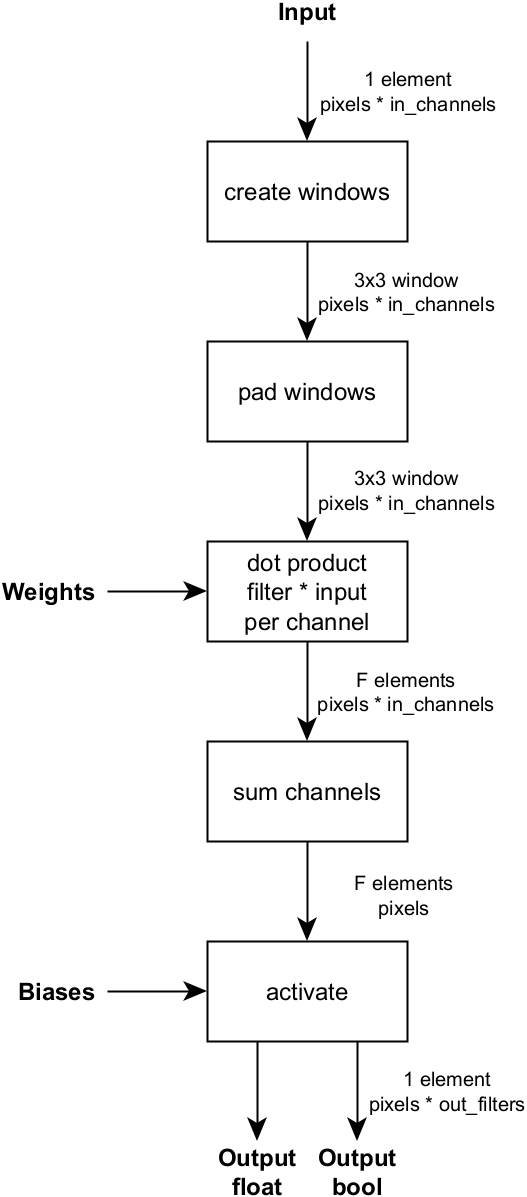
\includegraphics[width=0.406\textwidth]{Images/block_diagrams/conv2d_fp_mc.png}
        \decoRule
        \caption[Conv2D forward propagation block diagram]{Block diagram of the 2D convolution forward propagation. F is the number of filters. The data types of the internal streams with the total data passed are shown. }
        \label{fig: Conv2D forward propagation block diagram}
\end{figure}

The transformation from software to HLS hardware implementation is shown in the following pseudocode:
\begin{algorithm}[H]
    \caption[Conv2d Software implementation.]{2D Convolution: Software implementation.}
    \label{alg:Conv2d_SW}
    \begin{algorithmic}
        \Function {\textbf{SW Implementation}:}{}
            \For {$p$ in pixels}
                \For{$o$ in output channels}
                    \For{$i$ in input channels}
                        \State $out[p][o] \pluseq filter[o][i] * in[p][i]$
                    \EndFor
                    \State $out[p][o] = activate(out[p][o])$
                \EndFor
            \EndFor
        \EndFunction
    \end{algorithmic}
    $out[p][o]$, $filter[o][i]$ \& $in[p][i]$ have the dimensions of the filter. They can be multiple dimension arrays.
\end{algorithm}

\begin{algorithm}[H]
    \caption[Conv2d Software to HLS Transformation.]{2D Convolution: Software to HLS Hardware Transformation.}
    \label{alg:Conv2d_SW_to_HLS}
    \begin{algorithmic}
        \Function {\textbf{Step 1}: Transpose output channels dimension from time to space.}{}
            \For {$p$ in pixels}
                \For{$i$ in input channels}
                    \State $out[p][0] \pluseq filter[0][i] * in[p][i]$
                    \State $out[p][1] \pluseq filter[1][i] * in[p][i]$
                    \State $\ldots$ \Comment{output channel times}
                \EndFor
                \State $out[p][0] = activate(out[p][0])$
                \State $out[p][1] = activate(out[p][1])$
                \State $\ldots$ \Comment{output channel times}
            \EndFor
        \EndFunction
        
        \Function {\textbf{Step 2}: Split multiplications, additions \& activations in distinct functions.}{}
        \EndFunction
        \Function {Func A:}{}
            \For {$p$ in pixels}
                \For{$i$ in input channels}
                    \State $A[0] = filter[0][i] * in[p][i]$
                    \State $A[1] = filter[1][i] * in[p][i]$
                \State $\ldots$ \Comment{output channel times}
                    \State Write $(A[0], A[1], \cdots)$ to $streamA$
                \EndFor
            \EndFor
        \EndFunction
        \Function {Func B:}{}
            \For {$p$ in pixels}
                \For{$i$ in input channels}
                    \State Read $(A[0], A[1], \cdots)$ from $streamA$\
                    \State $B[0] \pluseq A[0]$
                    \State $B[1] \pluseq A[1]$
                    \State $\ldots$ \Comment{output channel times}
                \EndFor
                \State Write $(B[0], B[1], \cdots)$ to $streamB$
            \EndFor
        \EndFunction
        \Function {Func C:}{}
            \For {$p$ in pixels}
                \State Read $(B[0], B[1], \cdots)$ from $streamB$
                \State $out[p][0] = activate(B[0])$
                \State $out[p][1] = activate(B[1])$
                \State $\ldots$ \Comment{output channel times}
            \EndFor
        \EndFunction
    \end{algorithmic}
\end{algorithm}

\begin{algorithm}[H]
    \caption[Conv2d HLS implementation.]{2D Convolution: HLS implementation.}
    \label{alg:Conv2d HLS}
    \begin{algorithmic}
        \Function {\textbf{Step 3}: Make output channels dimension flexible between time \& space using HLS tools.}{}
        \EndFunction
        \Function {Func A:}{}
            \For {$p$ in pixels}
                \For{$i$ in input channels}
                    \State \#pragma HLS PIPELINE II=flexible
                    \For{$o$ in output channels} \Comment{If II=1 loop is flattened}
                        \State $A[o] = filter[o][i] * in[p][i]$
                    \EndFor
                    \State Write $(A[0], A[1], \cdots)$ to $streamA$
                \EndFor
            \EndFor
        \EndFunction
        \Function {Func B:}{}
            \For {$p$ in pixels}
                \For{$i$ in input channels}
                    \State \#pragma HLS PIPELINE II=flexible
                    \State Read $(A[0], A[1], \cdots)$ from $streamA$
                    \For{$o$ in output channels} \Comment{If II=1 loop is flattened}
                        \State $B[o] \pluseq A[o]$
                    \EndFor
                \EndFor
                \State Write $(B[0], B[1], \cdots)$ to $streamB$
            \EndFor
        \EndFunction
        \Function {Func C:}{}
            \For {$p$ in pixels}
                \State Read $(B[0], B[1], \cdots)$ from $streamB$
                \For{$o$ in output channels}
                    \State $out[p][o] = activate(B[o])$
                \EndFor
            \EndFor
        \EndFunction
    \end{algorithmic}
\end{algorithm}

The overall scheme is designed to maximize the data reuse providing maximum parallel data to the processing element, with minimum use of memory. Back propagation and gradient calculation follow the same logic with a few minor differences:

In back propagation, the input is the activated output gradients. To activate them, the system need to remember which neurons fired during forward propagation, as shown in figure \ref{fig: CNN dataflow}. Furthermore, the biases are not used, and the channel/filter dimensions are reversed. Finally the output are the gradients of the layer's input.

The processing element of the gradient calculation differs more. Instead of using the weights to calculate the outputs, the outputs are used to calculate the weight gradients. Furthermore, finding the bias gradients is trivial, as they are equal with the sum of all output gradients of their filter.

\begin{figure}[H]
    \centering
        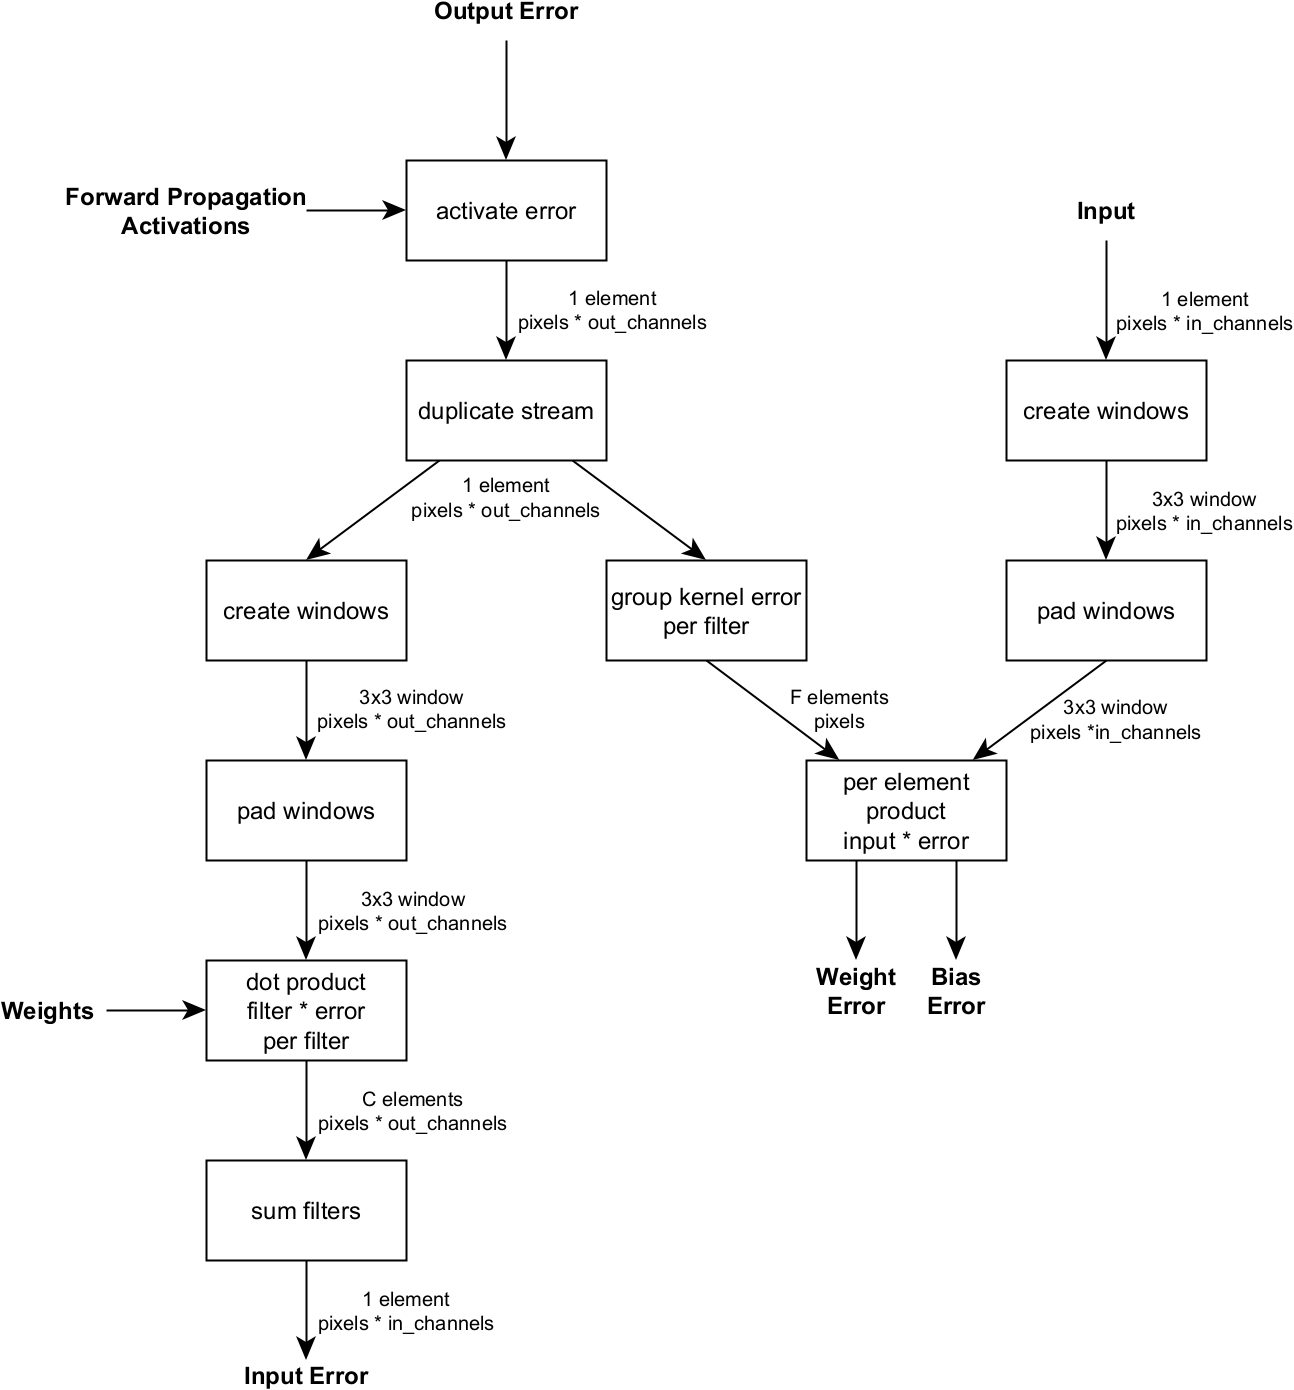
\includegraphics[width=1\textwidth]{Images/block_diagrams/conv2d_bp_cg_mc.png}
        \decoRule
        \caption[Conv2D back propagation block diagram]{Block diagram of the 2D convolution back propagation. F is the number of filters, C is the number of input channels. The data types of the internal streams with the total data passed are shown. }
        \label{fig: Conv2D back propagation block diagram}
\end{figure}

\subsection{2D Max-Pooling Layers}
The 2D Max-Pooling layers are implemented using the same logic as the 2D convolutional layers, albeit with a few major differences. First of all the window is 2x2 is size, and with a stride of 2. As a result, each window contains exclusive data, and an output can only be obtained with four inputs.

\begin{figure}[H]
    \centering
        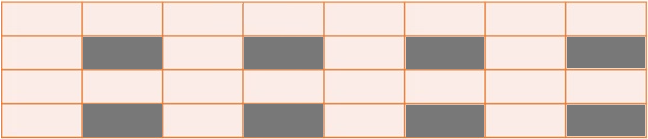
\includegraphics[width=1\textwidth]{Images/diagrams/line_buf_maxp.png}
        \decoRule
        \caption[Line Buffers, Max-Pool]{Line Buffers, Max-Pool: Grey pixels represent which inputs will trigger an output generation.}
        \label{fig: Line Buffers Max-Pool}
\end{figure}

Figure \ref{fig: Line Buffers Max-Pool} demonstrates the Max-Pool layer's uneven output generation, an unavoidable issue of any algorithm with stride greater than one. Following hardware does not operate while there are no data available, which is a problem in a FPGA design, as idle hardware indicates wasted hardware space. By raising the Iteration Interval (II) of the following hardware functions and properly calibrating the size of internal FIFO streams, the constant operation of the entire system is ensured.

The processing component of forward propagation is quite simple, as the output is the highest value in each window. It is important to note that the output's spatial dimensions are two times smaller than those of the input. Even more straightforward is back-propagation, in which the error back-propagates towards the maximum of each window. All other connections are assigned zero error gradients.

\subsection{Dense \& Softmax Layers}
The implementations of the dense and Softmax layers are simple and fairly similar. They are made up of two components: matrix multiplication of their inputs and weights and their respective activation function. In back-propagation and gradient calculation, the output error is activated before used as the input, with the input and variable gradients being the outputs.

The most crucial aspect of their design is ensuring that the hardware functions are constantly operating. To accomplish this, a streaming architecture, that reads and writes inputs and outputs serially and only once, is used. Important to note is that the Softmax activation requires all the inputs to be received before calculating any output, meaning that for an example back-propagation can not start until forward propagation is fully completed.

\subsection{Gradients Calculation Pipeline} % TODO: find better title
A major advantage of FPGA accelerators is that multiple hardware functions operate simultaneously, if the implemented algorithm allows. This holds true for most of the design. As an example, The first maxpool layer requires four inputs to generate the first output. These inputs have being generated by the first convolutional layer before a training data-point is fully loaded and processed. Thus the first two layers can operate simultaneously. % hardware function can operate simutanusly

On the other hand, the Softmax layer, which is the last step of the forward propagation, operates like a barrier. Due to the nature of the algorithm, to produce its feature map, all inputs must first be collected. As a result, for a single training data-point, the forward propagation must be completed before the back propagation begins. % softmax is a barrier

As such, the sequential semantics must be preserved, and the pipeline is implemented with a dataflow region that follows the control-driven task-level parallelism paradigm. This means that a subsequent function can start before the previous finishes and multiple functions can start and operate simultaneously. All tasks and channels are instantiated and connected explicitly. Furthermore, the inputs and outputs of the tasks are of stream type or stable memory arrays. % implementation

In this paradigm, the task with the highest latency typically determines the overall latency. Due to the existence of the Softmax barrier, for a single data input, forward propagation tasks can not operate simultaneously with tasks after it. As a result, the minimum overall latency equals the highest task latency before the barrier plus the highest task latency after it. % implementation barrier clash, overall latency

Figure \ref{fig: Gradients Calculation Pipeline Block Diagram} shows in detail the developed dataflow region that generates the weight and bias gradients. The heavy use of auxiliary data transformation functions, such as create windows and stream, is evident. These functions consume almost no hardware when synthesized, and add near zero latency. % auxiliary functions

Furthermore, several data streams skip hardware functions and layers. This could introduce stalls and ultimately deadlocks. To address this issue, hardware functions are implemented as free running pipelines $($FRPs$)$, when possible. Such implementations significantly reduce the possibility of a stall, by continuing to operate even when no input data are available or the output streams are full. % using frp and what they are

\begin{figure}[H]
    \centering
        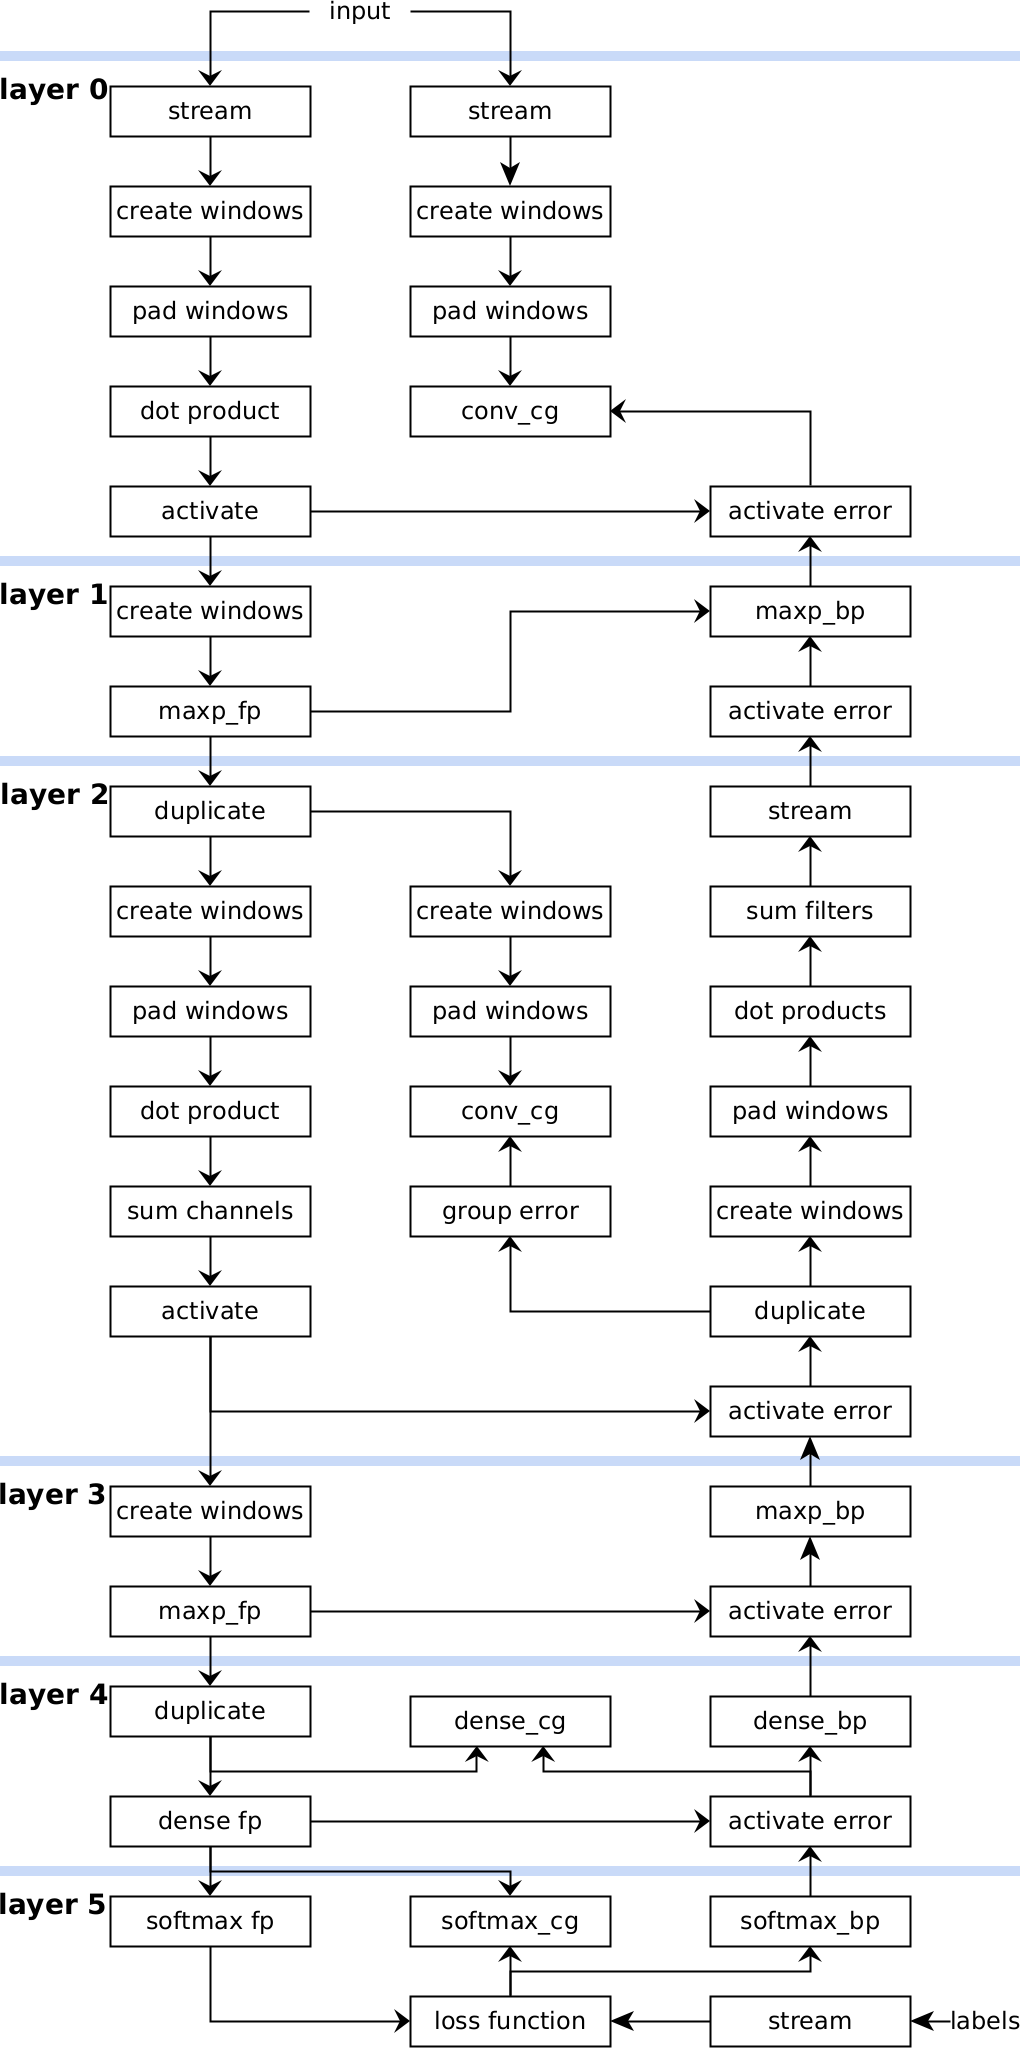
\includegraphics[height=0.95\textheight]{Images/block_diagrams/process_batch.png}
        \decoRule
        \caption[Gradients Calculation Pipeline Block Diagram]{Block diagram of the pipeline that generates the gradients. Inputs/Outpouts are not shown. Arrows represent data streams.}
        \label{fig: Gradients Calculation Pipeline Block Diagram}
\end{figure}
Using FRPs comes with multiple restrictions, a strict coding style is required, and MAXI ports are not supported. For hardware functions that read or write data from MAXI ports or can not adhere to other restrictions, flushable pipelines (FLPs) are used instead. They achieve the same goal as FRPs, but by instantiating multiple copies of the pipeline and executing them independently. As a result, the design is robust against any unpredictable stalls that MAXI ports may introduce. % FLPs and result

\subsection{Hardware Streams}
All communication between the hardware functions is facilitated with the stream implementation provided by the Vitis HLS library "hls\_stream.h". Hardware functions stall when an output stream is full, making the overall architecture inefficient. It is crucial to prevent this by determining the proper depth of the streams.

In most cases, this is trivial as they link sequential functions in a dataflow region where the consumer can instantly begin utilizing any data written by the producer. Then the major factor of the depth is the II of the connected functions. For most stream, a depth of two is sufficient.

More consideration is required about the streams that skip parts of the function chain. Due to the Softmax barrier, forward propagation of a sample is completed before its back propagation begins, thus all their data are produced before any of them is consumed. As such, their minimum depth is equal with the data produced by a single input sample.

To determine the ideal depths, an iterative optimization approach has typically been used. The Vitis HLS environment offers a variety of simulation tools that generate a number of useful statistics, such as the amount of clock cycles that each function stalls and whether or not a stream becomes full. Monitoring these when testing, enables calibrating the depths to ensure the stable flow of the pipeline, while not wasting hardware space in unnecessarily large streams.

\subsection{Batching Inputs}
As already explained, not all hardware functions can run concurrently for a single input sample. This issue is mitigated through batching input samples, where while an input runs through back-propagation, the next one is used in forward propagation. % description

\begin{figure}[H]
    \centering
        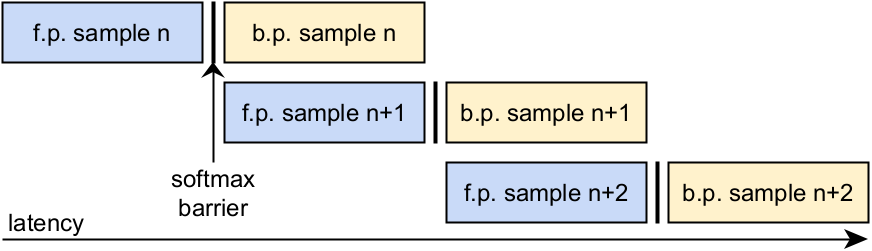
\includegraphics[width=\textwidth]{Images/diagrams/pipeline_under_batching.png}
        \decoRule
        \caption[Pipeline with batching latency]{ Latency of the pipeline under batching.}
        \label{fig: Batching Pipeline latency}
\end{figure}

With both sub-regions of the the pipeline having the same latency, the expected overall latency for a dataset without batching is defined as: % math
\begin{equation}
L_{dataset} = \sum^{samples}( L_{fp} + L_{bp} ) = 2 \cdot samples \cdot L_{fp/bp}
	\label{eqn: latency dataset no batching}
\end{equation}

With batching enabled, the latency of the dataset is transformed as:
\begin{equation}
    \begin{gathered}
        L_{dataset} = \sum^{\substack{batches\\ per\ dataset}}\sum^{\substack{samples\\ per\ batch}}( L_{fp/bp} + 1 ) =\\
        \frac{samples}{size_{batch}} \cdot size_{batch} \cdot ( L_{fp/bp} + 1 ) =\\
        samples \cdot ( L_{fp/bp} + 1 )
    \end{gathered}
	\label{eqn: latency dataset with batching}
\end{equation}

With Vitis HLS, implementing batching on each individual hardware function is quite trivial. Encapsulating their C++ definitions in a loop of the same size as the desired batch, is sufficient. % implementation

Further though must be given to the size of the streams connecting functions of the forward propagation with functions after the barrier. The producer functions will block until the consumer functions clear some space in the stream if the minimal depth is used as mentioned in the preceding section. Depending on the minimal latency between the producer and the consumer, this can be avoided by increasing the depth by 0.5 to 1 times.

\subsection{Updating Variables}
Based on the produced gradients, the variables of the ANN are updated in a second dataflow region. Due to the independence of all weights and gradients, the process is relatively straightforward. The basic gradient descend algorithm is used and the learning rate is supplied by the driver program. Thus, latency and hardware usage are the only criteria for the applied parallelism.

\subsection{Data Movement \& Storage}
Under the Vitis flow, AXI streams are unavailable for the ZCU102, thus memory mapping is used to transfer data from general memory to the PL and vice versa. These data are the input samples and labels, as well as the variables of the ANN. Appropriate data mover functions have been developed. % gmem <-> accel, which data

In Vitis HLS, arrays are implemented as continuous memory spaces with one or two ports, and only a limited amount of data can be read or written per cycle. To increase data accesses per cycle, the arrays are partitioned with the appropriate HLS directive \emph{ARRAY\_PARTITION}. The HLS tool splits the initial arrays to smaller ones, whose size and shape depend on the parameters of the corresponding directives. % array partition

The weights of the ANN are accessed in multiple functions of the first dataflow region and require special treatment. These arrays must be designated as shared using the directive \emph{STREAM} with the type parameter set to \emph{SHARED} in order for the design to be syntesizable. The tool then recognizes there are numerous consumers and multiplies the ports accordingly, without duplicating the array data. % shared arrays

For the weights of the second convolutional layer, this is insufficient. They are accessed by two functions with different access patterns. This issue can be resolved in two ways. The first one is satisfying both access patterns by increasing the partition factor and dimensions. This solution generate a huge amount of access ports, increasing hardware consumption unacceptably. More appropriate solution is creating two arrays with unique partitioning each. Albeit more memory is needed, the overall hardware usage is lower. % double arrays for layer 2 weights

When generating the gradients, the ANN's inputs, data and labels, are sent from global memory to the PL via AXI Master Adapter ports. In a dataflow region, each channel must have a single consumer, thus two ports are needed to propagate the input data to the two hardware functions that consume it. All ports are independent from one another by having their own dedicated bundles, thus enabling the simultaneous reading of all inputs. % dataflow inputs

The variable gradients are produced in the first dataflow region and consumed in the second, thus persistent saving in on-chip memory is necessary. The related arrays are not shared since their producers and consumers are in different regions, and can be implemented as streams or arrays, whichever is more convenient. % gradients

% \subsection{Minimizing Global Memory Accesses}
% bursting / port widening
% Rejected

\subsection{Top function}
To hold everything together, a top level function has been developed, whose signature operates as the API between PL and PS. Furthermore, it contains all the definitions of the memory structures, as well as the instantiations of the data movers and dataflow regions. Finally, to train on multiple batches, the dataflow regions are enclosed in a loop.

\begin{figure}[H] % TODO: remove the batch fetching
    \centering
        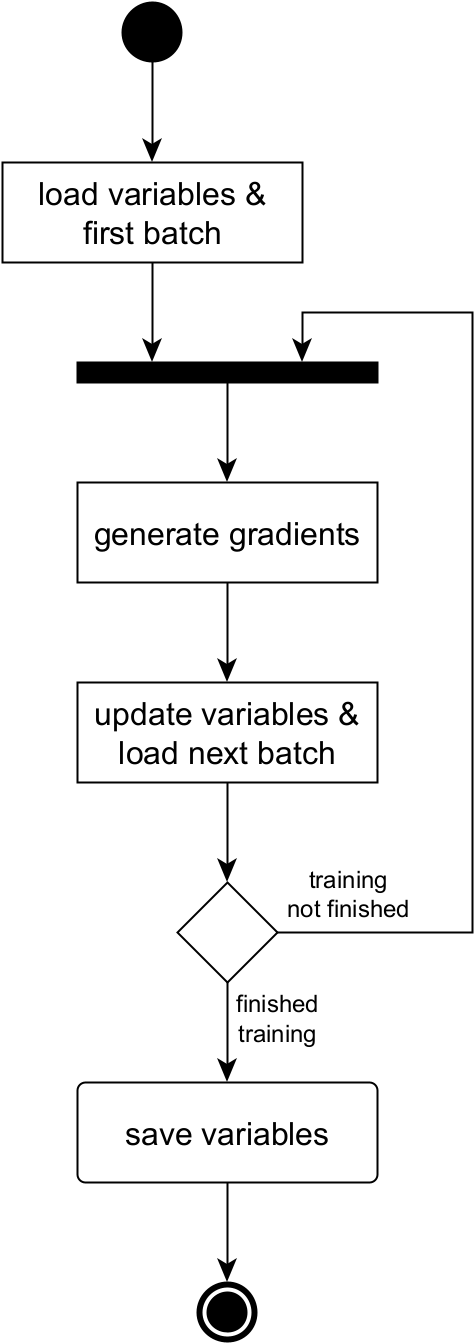
\includegraphics[height=0.5\textheight]{Images/block_diagrams/accel_top.png}
        \decoRule
        \caption[Top function]{Block diagram of the accelerator's top function.}
        \label{fig: top function}
\end{figure}

\section{Host Program}
The overall application uses Linux system calls, such as socket read and write. Thus a bare metal implementation is inadequate and a host program in the PS is required to drive the developed hardware design in the PL. This is achieved with the use of the XRT native C++ APIs \cite{XRT_Native_APIs}.

The flow of the driver code is as follows:
\begin{itemize}
    \item Open the device.
    \item Load the compiled and linked binary (XCLBIN) onto the device.
    \item Open the kernel loaded to the device with the XCLBIN.
    \item Create Buffer objects to transfer data to kernel inputs and outputs.
    \item Write data to the input buffers.
    \item Execute the kernel.
    \item Read data from the outputs buffers.
\end{itemize}

\chapter{Results}
\label{Chapter-Results}
This chapter has three aims. First, to quantify the performance of the FPGA implementation of the ANN and analyze its resource consumption and timing. Second, to compare it will equivalent implementations on other technologies. Final and main goal, to study the interaction and discover any possible synergies or conflicts between the two technologies under focus, namely FL and FPGA. % aims

It should be noted that the following timings were produced through actual runs in a real FPGA. In the following subsections it is explained in detail how they were generated and what they actually mean.

\subsection*{Performance Metrics}

\subsubsection{Latency}
Latency, is the required time to complete a single task. In this work, latency can be the time taken to process a single image, a batch of images, a dataset of images, etc. % what is latency

\subsubsection{Throughput}
Throughput is generally referred to as the quantity of tasks completed in a given amount of time. The rate at which something is processed increases with throughput. Throughput in this work is referred to as the number of images processed per second. % what is throughput
\begin{equation}
	Throughput \coloneqq \frac{Images}{Time (sec)}
	\label{eqn: Throughput definition}
\end{equation}

\section{FPGA Implementation Analysis}

\subsection{Resource Utilization Analysis}
Although consisting of only $\sim$105000 variables and 6 layers, the implemented ANN consume a lot of resources. It has full floating point accuracy, back-propagation is employed for training, and the SGD optimization algorithm makes use of momenta. When applied in programmable logic, all of these techniques are known to significantly increase resource usage. Table \ref{table: Resource Utilization} depicts the utilization of the major resources after synthesis, place and route; according to the Vitis IDE. % resource consumpion
\begin{table}[H]
    \center
    \begin{tabular}
        { | l | r | r | r | }
        \hline
        Resource & Utilization & Available & Utilization \%\\
        \hline
        LUT      & 161274 & 274080 & 58.84\\
        LUTRAM   &  14270 & 144000 &  9.91\\
        FF       & 260050 & 548160 & 47.44\\
        BRAM     &    573 &    912 & 62.83\\
        DSP      &    854 &   2520 & 33.89\\
        \hline
    \end{tabular}
    \caption[Resource Utilization]{Post place \& route resource utilization.}
    \label{table: Resource Utilization}
\end{table}
The highest use rate is observed on the BRAM. It is intrinsically tied to the size of the ANN due to three key factors. Firstly, to enable the quickest access to the ANN's variables, they are stored in on-chip memory. Furthermore, the back-propagation algorithm demands the temporary storage of all data that bypass hardware functions. Lastly, between each batch update, the SGD algorithms' momenta must be saved. %BRAM comment

The utilization of the rest of the PL is affected mostly on the desired accuracy and the applied parallelism. Using single precision floating points is more resource demanding than using half precision and less than using double precision. Although it appears there is space to improve parallelism, the benefits diminish the more that this is done. Most crucially, timing-based constraints rather than resource-based constraints are the biggest barriers to it. %the rest comment

\subsection{Timing Analysis}
A thorough analysis of the implementation's timings is required to to assess its performance, identify delays and limitations, as well as enable future improvements. This section provides a breakdown of the relevant latencies. The following formulas and results have been confirmed by experiments on the ZCU102. % why analize timing

\subsubsection{Overall Latency}
From the point of view of the host program, the overall latency of training can be broken down as follows; writing the variables in global memory, calling the accelerator, waiting for the accelerator to return, and finally read the produced variables from the global memory. % host latency
\begin{equation}
	Host_{latency} = GMEM_{write} + Accel_{call} + Accel_{wait} + GMEM_{read}
	\label{eqn: host program, training latency}
\end{equation}
Important to note, all parts involve system calls to the operating system, which can introduce a small variance in their latency. Additionally, in the case of the FL client with the map API, the latency of accessing the global memory is hidden under the FL operation, as the socket reads and writes there directly. % comments

\subsubsection{Accelerator's Latency}
Accountable for the majority of the overall latency is waiting for the accelerator to finish running. As observed in figure \ref{fig: top function}, its operation consists of initializing its on-chip local memory, calculating the gradients, updating the variables, and finally writing the final variables to the global memory. % parts of accel latency

The first and the last segments are executed only once and they are independent of any variable such as the size of the dataset used for training. In contrast, the two dataflow regions, generating the gradients and updating the trainable variables, are repeated multiple times depending on the number of training epochs and the number of batches in the dataset. in more detail: % what is repeated
\begin{equation}
    Accel_{latency} = I + e \cdot \frac{d}{b} [ G(b) + U ] + S
    \label{eqn: Accel, training latency}
\end{equation}
Where:
\begin{conditions}
    I & initialize inputs\\
    e & training epochs\\
    d & dataset size\\
    b & batch size\\
    G & calculate the gradients\\
    U & update trainable variables\\
    S & Save final variables\\
\end{conditions}
Calculating the gradients is done using the long and complex pipeline depicted in figure \ref{fig: Gradients Calculation Pipeline Block Diagram}. It has significant wind-up and wind-down latencies and its total run-time is dependent on the batch size. % gradients calculation analysis
\begin{equation}
    G(b) = G_{up} + b \cdot E + G_{down}
    \label{eqn: Gradients pipeline, training latency}
\end{equation}%
Where:
\begin{conditions}
    G_{up} & latency to wind-up the pipeline\\
    G_{down} & latency to wind-down the pipeline\\
    E & latency added by one example\\
\end{conditions}
Thus, the latency of the accelerator can better be described as:
\begin{equation}
    Accel_{latency} = I + S + e \cdot d [ E + \frac{ G_{up} + G_{down} + U }{b} ] % 24613 + 60000 [ 33320 + ( 35310 + 25121 )/b ]
    \label{eqn: Accel, training latency, complete}
\end{equation}
$U$, as described in section \ref{sec:Updating_Variables}, is completely elastic and the main target when optimizing for small batches.

Through analyzing the Vitis reports, exact numbers can be assigned on each constant. For a single pass through the whole dataset $( e=1, d=60000 )$ and a clock speed of $4.08 ns (\sim245MHz)$, the equation transforms to: % function with numbers
\begin{equation}
    Accel_{latency} = 8.157 + \frac{ 14.794 }{b} (sec) % 1999224613 + 3625860000/b 
    \label{eqn: accel, training latency in ms}
\end{equation}
\subsubsection{Constrains}
\label{Constrains}
According to equation \ref{eqn: Accel, training latency, complete}, the latency introduced by each example (E) is the most important constant. Accountable for that is the dataflow region shown in figure \ref{fig: Gradients Calculation Pipeline Block Diagram}, thus received most of the optimization attention. Better performance is restricted mostly by a single issue caused by the HLS tool, affecting clock speed and the total operating clock cycles. % importance of E and issues

The slowest function of a dataflow region determines its overall latency. In this case, it is the \textit{sum filters} in the back-propagation of the second convolutional layer. Per example, it has 14$\times$14 inputs with 32 input and 16 output channels. The outputs are independent from each other and are calculated in parallel. Thus, 16 accumulators that reset every 32 cycles are needed. % where is problem

Unfortunately, in the latest versions of the Vitis HLS, the tool can not deduce that the \textit{facc} operator is the optimal choice if its accuracy has not been set to low. Instead, when normal accuracy is requested, it implements the slower \textit{fadd} operator, which forces an II of 5 cycles and a clock speed of 245MHz. As a result, the latency of a single example is at least 31360 cycles. % what is the problem and what it affects

The next slowest functions are the \textit{create windows} hardware functions in the convolutional and maxpool layers (layers 0 to 3). While they are simple data transformation, the HLS tool encounters some difficulty in implementing them efficiently, as they are composed mostly of control logic. Still, it is able to synthesize them with a clock of over 300 MHz.% Furthermore, it is unable to always synthesize them with a free running pipeline, requiring deeper input and output streams to guarantee robustness against random stalls. % next slowest

Both cases are byproducts of using HLS tools. If just the \textit{facc} bug is avoided, the clock can be immediately increased by 55MHz. Without trying to improve the II of the function, the latency equation transforms to: % Creating these two function using RTL, would greatly improve the overall performance.  % change with facc
\begin{equation}
    Accel_{latency} = 6.664 + \frac{ 12.086 }{b} (sec) % 1999224613 + 3625860000/b
    \label{eqn: Accelerator with facc, training latency in ms}
\end{equation}
Visualizing the equations \ref{eqn: accel, training latency in ms} \& \ref{eqn: Accelerator with facc, training latency in ms} in the diagram \ref{fig: accel latency}, shows that their second part is insignificant for batches of over 100 images. In contrast, the first part is unavoidable and sets a base latency regardless of the batch size. % visualize
\begin{figure}[H]
    \center
    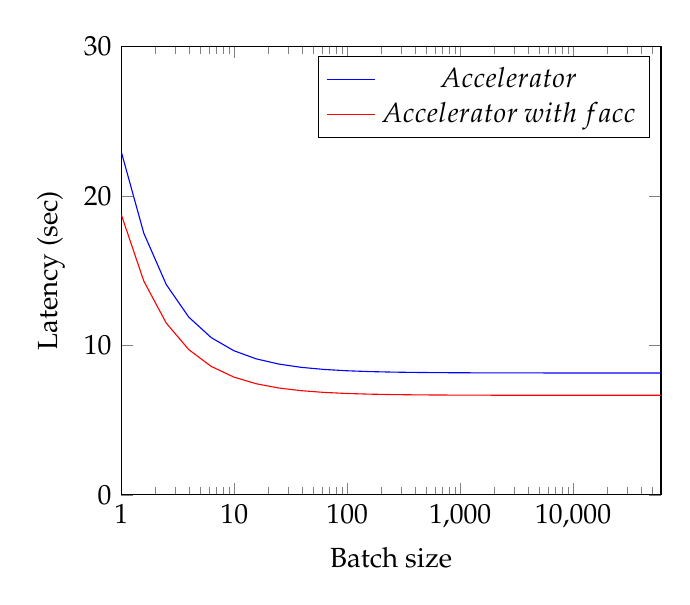
\begin{tikzpicture}
        \begin{axis}[
            xmode = log,
            log ticks with fixed point,
            ymin = 0,
            ymax = 30,
            xmin = 1,
            xmax = 60000,
            ylabel = Latency (sec),
            xlabel = Batch size
        ]
            \addplot[ domain = 1:60000, color = blue ] { 8.156836421 + 14.793508800 / x };
            \addplot[ domain = 1:60000, color = red ] { 6.664082036 + 12.086199879 / x };
            \addlegendentry{$Accelerator$}
            \addlegendentry{$Accelerator\:with\:facc$}
        \end{axis}
    \end{tikzpicture}
    \caption[Accelerator's latency per batch size]{Latency with and without the facc module.}
    \label{fig: accel latency}
\end{figure}

\subsection{Power Consumption Analysis}
The average power consumption of the design can be reliably estimated by the Xilinx tools. This report was generated post-implementation and is shown in figure \ref{fig: power}. A breakdown of the consumption per PL element can be seen.

\begin{figure}[H]
    \centering
        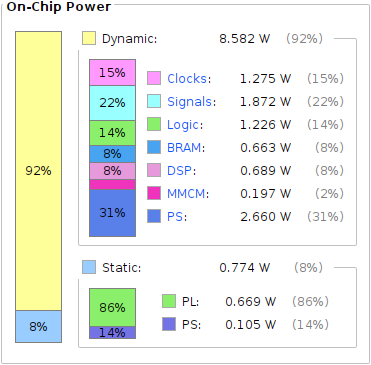
\includegraphics{Images/power.png}
        \decoRule
        \caption[Power Estimation]{Post-implementation power estimation of the accelerator.}
        \label{fig: power}
\end{figure}

The average consumption is stated as 9.356 W, with the PL accountable for the majority of it. This is to be expected, as the PS part of the accelerator mostly does nothing while waiting for the PL part to finish. In practice, most of the PS consumption is sourced from the of-chip memory used.

\section{Comparison with Other Technologies}
To form an opinion on the efficiency of the FPGA implementation, a proper comparison is required. Thus, the ANN is also trained on CPU and GPU using TensorFlow. As metrics, the latency of a training epoch and the overall throughput are used.

\subsection{Specification of Compared Platforms}
\subsubsection{Intel Core i7-9750H}
Released in mid 2019, the i7-9750H is a high end CPU for laptops. Based on the Coffee Lake architecture and manufactured with the 14nm++ process, it provides a wide array of technologies such as Hyper-Treading and SIMD Instruction Set Extensions, making it suitable for training the ANN under consideration. Furthermore, TensorFlow has been compiled with AVX instructions enabled. % CPU
\begin{table}[H]
    \center
    \begin{tabular}
        { l | l }
        Core / Threads & 6 / 12\\
        Clock Frequency & 2.6 - 4.5 GHz\\
        Cache & 12 MB Intel Smart Cache\\
        Supplied Memory & 16GB DDR4-2666\\
        Max Memory Bandwidth & 41.8 GB/s $\times$ 2 channels\\
        Instruction Set Extensions & SSE4.1, SSE4.2, AVX2\\
        Average Power Consumption & 45 W\\
    \end{tabular}
    \caption[i7-9750H specifications]{i7-9750H specifications \cite{i7-9750H}.}
    \label{table: i7-9750H}
\end{table}

\subsubsection{Nvidia GTX 1660 Ti}
While released in early 2019 as mobile platform (laptops, tablets, etc.) GPU, is more than capable for training ANNs like the one under investigation. Its relevant specifications are shown on the following table. % GPU
\begin{table}[H]
    \center
    \begin{tabular}
        { l | l }
        CUDA cores & 1536\\
        Clock Speed & 1500 - 1770 MHz\\
        Memory Configuration & 6GB GDDR6, 1500 MHz\\
        Memory Interface & 192-bit\\
        Memory Bandwidth & 288 GB/s\\
        Single Precision Compute Power & 5437.44 GFLOPS\\
        Compute Capability & 7.5\\
        Average Power Consumption & 120 W\\
    \end{tabular}
    \caption[GTX 1660 Ti specifications]{GTX 1660 Ti specifications \cite{GTX1660Ti}.}
    \label{table: GTX1660Ti}
\end{table}

\subsection{Latency Comparison}

\begin{figure}[H]
    \center
    \begin{tikzpicture}
        \begin{axis}[
            xmode = log,
            log ticks with fixed point,
            ymin = 0,
            ymax = 110,
            xmin = 1,
            xmax = 60000,
            ylabel = Latency (sec),
            xlabel = Batch size,
            scale = 1.25,
            no markers
        ]
            \addplot[ domain = 1:60000 , color = blue ] { 8.166836421 + 14.793508800 / x };
            \addlegendentry {$FPGA$}
            
            \addplot+ [ forget plot , name path=upper_gpu , draw=none ] table[ smooth , tension=.8 , x=batch_size , y=latency_max ] {data/gpu_latency_per_batch_size.dat};
            \addplot [ name path=lower_gpu , color=red ] table[ smooth , tension=.8 , x=batch_size , y=latency_min ] {data/gpu_latency_per_batch_size.dat};
            \addplot+ [ forget plot , fill=red!25 ] fill between[ of=upper_gpu and lower_gpu ];
            \addlegendentry {$GPU$}

            \addplot+ [ name path=upper_cpu , color=green ] table[ smooth , tension=.8 , x=batch_size , y expr = ( \thisrow{latency_max} + \thisrow{latency_min} ) / 2 ] {data/cpu_latency_per_batch_size.dat};
            \addlegendentry {$CPU$}
        
        \end{axis}
    \end{tikzpicture}
    \caption[FPGA, GPU, CPU latency comparison]{Latency of training for a single epoch on FPGA, GPU and CPU}
    \label{fig: FPGA CPU GPU latency}
\end{figure}

Due to the CPU's fluctuating clock speed and caching architecture, training latency has a slight variance. This effect is considerably more pronounced on the GPU, as it also copy the training dataset and the ANN's variables to its dedicated memory, during the first epoch. % variance CPU, GPU

On the FPGA, however, training latency is practically deterministic. The only variance that it encounters, is produced by the system calls and is less than 10 ms. Such effects should be noted as this work also considers on-edge devices, where the training algorithm may not have complete control over them and their environment is not always in an ideal state. % variance GPU

Performance wise, according to figure \ref{fig: FPGA CPU GPU latency}, the FPGA implementation outperforms in training with small batches, but is overtaken by the GPU when their size is larger than or equal to 15 examples. Training on CPU is consistently slower than the other technologies.

It should be noted that the GPU is unable to perform non-Stochastic Gradient Descent, where the whole dataset is concatenated in a batch. TensorFlow can not obtain enough GPU dedicated memory and crashes. Due to non-determinism in memory management, this can also occur for SGD with batches of more than 15000 samples. In on-edge devices, such effects are expected to become more noticeable, due to the FL algorithm's limited control.

\subsection{Throughput Comparison}
\begin{figure}[H]
    \center
    \begin{tikzpicture}
        \begin{axis}[
            ymode = log,
            xmode = log,
            % log ticks with fixed point,
            ymin = 100,
            ymax = 100000,
            xmin = 1,
            xmax = 60000,
            ylabel = Throughput (Images/sec),
            xlabel = Batch size,
            scale = 1.25,
            no markers,
            legend pos = south east
        ]
            \addplot[ domain = 1:60000 , color = blue ] { 60000 / ( 8.166836421 + 14.793508800 / x ) };
            \addlegendentry {$FPGA$}
            
            \addplot+ [ color=black ] table[ smooth , tension=.8 , x=batch_size , y expr={ 60000 / \thisrow{latency_max} } ] {data/gpu_latency_per_batch_size.dat};
            \addlegendentry {$GPU$, worst}
            
            \addplot+ [ color=red ] table[ smooth , tension=.8 , x=batch_size , y expr={ 60000 / \thisrow{latency_min} } ] {data/gpu_latency_per_batch_size.dat};
            \addlegendentry {$GPU$, best}

            \addplot+ [ color=green ] table[ smooth , tension=.8 ,
                x=batch_size ,
                y expr={ 60000 / ( ( \thisrow{latency_max} + \thisrow{latency_min} ) / 2 ) } ] 
                {data/cpu_latency_per_batch_size.dat};
            \addlegendentry {$CPU$}
        
        \end{axis}
    \end{tikzpicture}
    \caption[FPGA, GPU, CPU throughput comparison]{Throughput of FPGA, GPU and CPU implementations}
    \label{fig: FPGA CPU GPU throughput}
\end{figure}
Similar observations can be made by comparing the throughput of the implementations in figure \ref{fig: FPGA CPU GPU throughput}. Although the FPGA starts from more than 2600 images per second, its performance plateaus at around 7500. In contrast, the GPU can only achieve ~600 images per second with single image batches, but reaches a maximum throughput of 50000 when using huge batches.

\subsection{Power Consumption Comparison}
Table \ref{table: power} presents the power consumption of the three implementation. An actual system with the CPU or GPU implementation, would require other components to operate, e.g. a motherboard. In contrast, the FPGA-based implementation is aimed for the ZCU102, which is an SoC, and requires no other components. This is a gross comparison, and aims to give a general idea of their differences.
\begin{table}[H]
    \center
    \begin{tabular}
        { | c | c | c | }
        \hline
        CPU & GPU & FPGA\\
        \hline
        53 W & 120 W & 9.356 W\\ 
        \hline
    \end{tabular}
    \caption[Power Consumption]{Power consumption of the three implementations.}
    \label{table: power}
\end{table}
Although the CPU's average power usage is listed as 45 W, during actual runs it rises to 53 W due to clock frequency boosting. The FPGA consumes \(5.67\times\) less power than the CPU and \(12.83\times\) less power than the GPU.


\section{FL \& FPGA Interaction Analysis}
\subsection{Methodology}
The main objective of this study, to investigate how FL and FPGAs interact, is explored in this section. Merely comparing the throughput of the implementations is inadequate since, as demonstrated in chapter \ref{Chapter-Robustness-Analysis}, the number of global epochs depends on a multitude of factors. The batch size is the element that has the greatest impact on both FL and local training. As a result, it is the central factor of the experiments. % objective, why focus on batch size

Another factor that has a significant impact is the LR degradation. Through experimentation, the most effective tactic was determined to be decreasing a client's LR for each epoch it participates. Depending on the batch size, different rates of that decrease were the most efficient. To ensure fairness on the following experiments, they were repeated with various LR decay constants. In this section, the best results for each are presented. % LR decay

Having access to a single FPGA and a single GPU, makes running the algorithm in real time impossible, as it requires several devices. Instead, all processes, server and clients, run on the CPU to discover the number of required global epochs to reach a target accuracy, and then their training latency is replaced with that of the desired device. As all clients operate in parallel, the training latency is not depended on how many are used. % forced to simulate

The communication delay between server and clients is handled similarly. It is determined by multiplying the size of the messages with an expected communication speed. Generally, servers have high speed connections, up to 1 Gbps upload and download. In contrast, the connection speed of on-edge devices is multiple order of magnitude slower, and the deciding factor of the overall communication latency. % communication delay

Additional latencies, caused by synchronization or the computational part on the server, amount to just a few milliseconds per epoch and are consistent across all platforms. Therefore, they can conveniently be ignored. % other latencies

For the following tests, clients are configured with a download speed of 10Mbps and a upload speed of 1Mbps. Furthermore, the messages between client and server have a size of 3387808 bits. Considering that clients are operating in parallel, the latency of a Global Epoch can be described as: % GE latency
\begin{equation}
    \begin{gathered}
        GE_{latency} \simeq StoC_{latency} + LT_{latency} + CtoS_{latency}\\
                     = \frac{ StoC\_msg_{bits} }{ C\_down_{bps} } + LT_{latency} + \frac{ CtoS\_msg_{bits} }{ C\_up_{bps} }\\
                     = LT_{latency} + 3.7266 \: (sec) % 0.3388 + 3.3878
    \end{gathered}
    \label{eqn: Global Epoch Latency}
\end{equation}
Where:
\begin{conditions}
    LT & Local Training\\
    StoC & Server to Client\\
    CtoS & Client to Server\\
\end{conditions}

It should be noted that the results of the previous section can not be used in place of $LT_{latency}$. The size of the local datasets differs, depending on how the data are distributed across the clients. Thus, the latency of the local training has been re-measured for every platform. % lt remeasured

\subsection{IID} % TODO: replace X and Y with numbers
In the first experiment, the Fashion-MNIST dataset is split randomly and evenly across 10 clients. This is an IID distribution, in the sense that is used in relevant bibliography. All random factors, such as dataset distribution and client selection, have been seeded to remove their effects from the final results. % data, seeds

The model is trained with the FedAvg algorithm multiple times, once for each batch size that perfectly divides the local datasets. Out of the 10 clients, 5 of them are randomly selected to participate in each GE. The constant parameters of the experiment are listed in table \ref{table: ΙID experiment parameters}. % algorithm & parameters
\begin{table}[H]
    \center
    \begin{tabular}
        { | l | c | }
        \hline
        parameters & FedAvg\\\hline
        total clients   & 10\\\hline
        clients per GE  & 5\\\hline
        local epochs    & 1\\\hline
        initial LR      & 1e-2\\\hline
    \end{tabular}
    \caption[IID experiment parameters]{Constant parameters of the IID FL experiment.}
    \label{table: ΙID experiment parameters}
\end{table}

Each training run consists of 200 GEs or until it reaches the target accuracy of 91\%. In each GE, selected clients train their local models with their local datasets for 1 epochs. Figure \ref{fig: IID, GEs per batch size} shows the elapsed GEs to reach the target accuracy for every batch size.
\begin{figure}[H]
    \center
    \begin{tikzpicture}
        \begin{axis}[
            ybar,
            ylabel = Global Epochs,
            ymin = 0,
            ymax = 200,
            xlabel = Batch size,
            % xtick = data,
            symbolic x coords = {5,6,8,10,12,15,16,20,24,25,30,40,48,50,60,75,100,120,125,150,200},
            xtick style = {draw=none},
            scale = 1.25,
            enlarge x limits={abs=6pt},
        ]
            \addplot [ black , fill = blue!50 ] table [ x = batch_size , y = global_epochs] {data/IID_epochs.dat};
        \end{axis}
    \end{tikzpicture}
    \caption[ IID distribution, GEs per batch size ]{ GEs required to reach 91\% accuracy, when under IID distribution.}
    \label{fig: IID, GEs per batch size}
\end{figure}

Training with batch sizes of 4 or less, produces overfitted local models and renders the target accuracy unattainable. This problem could be alleviated by using a more sophisticated LR decay strategy or by distributing the dataset among more clients, but both are outside the scope of this work. % tiny batches

More interesting is the range of batch sizes from 5 to 50, where the target accuracy is reached in 30 to 60 GEs. Larger sizes increase the required number of GEs in a parabolic manner, and regardless how fast is the local training, the increase in communication most likely prohibits their use.

Figure \ref{fig: IID, total time} shows, per batch size, how much time is required to reach the target accuracy. The FPGA design is benchmarked with the best case of the GPU, where the dataset is already cached in its dedicated memory.  % final diagram what it is
\begin{figure}[H]
    \centering
    \addtolength{\leftskip} {-2cm} % increase (absolute) value if needed
    \addtolength{\rightskip}{-2cm}
    
    \begin{tikzpicture} [
        /pgfplots/every axis/.style = {
            ybar stacked ,
            bar width = 8pt,
            ymin = 0 ,
            ymax = 1000 ,
            ytick distance = 250 ,
            ylabel = Global Training time (sec) ,
            symbolic x coords = {5,6,8,10,12,15,16,20,24,25,30,40,48,50,60,75,100,120,125,150,200} ,
            enlarge x limits = 0.03 ,
            xtick = data,
            xtick style = { draw = none } ,
            xlabel = Batch size,
            width = 1.25 \textwidth ,
            height = 0.75 \textwidth ,
        }
    ]
        \begin{axis}[ bar shift = -4pt , ]
            \addplot [ black , fill = blue!75 ] 
                table [ 
                    y expr = { \thisrow{global_epochs} * ( 0.82568 + 1.47935 / \thisrow{batch_size} ) } , 
                    x = batch_size ,
                    meta expr = { \thisrow{global_epochs} * ( 0.82568 + 1.47935 / \thisrow{batch_size} ) } 
                ] {data/IID_epochs.dat};  % training cost

            \addplot [ black , fill = blue!25 ,
                point meta = y ,
                nodes near coords = \pgfmathprintnumber\pgfplotspointmeta ,
                every node near coord/.append style = {
                    font=\footnotesize ,
                    anchor = west ,
                    rotate = 90 ,
                    yshift = 4pt ,
                    /pgf/number format/.cd , precision = 0 ,
                }
            ] 
                table [ 
                    y expr = { \thisrow{global_epochs} * 3.73 } , 
                    x = batch_size , 
                    meta expr = { \thisrow{global_epochs} * 3.73 } ,
                ] {data/IID_epochs.dat}; % communication cost 
                \label{FPGA_iid} 
        \end{axis}
        
        \begin{axis}[ hide axis , bar shift = 4pt , legend pos = north west , ]
            \addplot [ forget plot , black , fill = red!75 ] 
                table [ 
                    y expr = { \thisrow{global_epochs} * ( \thisrow{gpu_lat_per_epoch} ) } , 
                    x = batch_size ,
                    meta expr = { \thisrow{global_epochs} * ( \thisrow{gpu_lat_per_epoch} ) } 
                ] {data/IID_epochs.dat};  % training cost

            \addplot [ black , fill = red!25 , 
                point meta = y ,
                nodes near coords = \pgfmathprintnumber\pgfplotspointmeta ,
                every node near coord/.append style = {
                    font=\footnotesize ,
                    anchor = west ,
                    rotate = 90 ,
                    yshift = -4pt ,
                    /pgf/number format/.cd , precision = 0
                }
            ]
                table [
                    y expr = { \thisrow{global_epochs} * 3.73 } ,
                    x = batch_size ,
                    meta expr = { \thisrow{global_epochs} * 3.73 }
                ] {data/IID_epochs.dat}; % communication cost

            \addlegendentry{GPU}
            \addlegendimage{ /pgfplots/refstyle=FPGA_iid }\addlegendentry{FPGA}
        \end{axis}
    \end{tikzpicture}
    
    \caption[ IID distribution, total time per GE ]{ Total wall-clock time to train with IID dataset distribution over 10 clients, per batch size. Darker colors = local training time, lighter colors = communication time. }
    \label{fig: IID, total time}
\end{figure}

It is apparent that communication, across all batch sizes, is the main contributor to overall latency. Considering that the dataset is split over 10 clients, 6000 examples for each one, there in not much training to be done per GE, rendering maximum throughput a secondary characteristic. Instead, the most important variables are the number of GEs and the minimum latency per GE. % com latency, what is more important

Batch sizes of 8 to 20 appear to be the sweet spot. In that range, either the FPGA has similar latency with the GPU, or it is slightly more efficient. With larger batches the GPU requires significantly less computing but, due to additional communication, the overall latency is abysmal. % best cases

\subsection{Non-IID}
Given that in real-world FL scenarios clients have different data collection and storage biases, it is exceptionally rare for the local datasets to be IID distributed. Every FL system should therefore be evaluated using non-IID data distributions. For this experiment, the FedAvg algorithm is employed, with all clients participating in every GE. % why non-IID & algorithm

The Fashion-MNIST dataset is divided among 5 clients, each of which is the exclusive owner of two labels. The first client owns all the examples with the first two labels, the second client has those with the next two labels, etc. This is a pathological non-IID distribution, arguably more unbalanced than real scenarios, but it is a great option to test the limits of the system. % data distribution

Like in the previous experiment, results are obtained with every batch size that perfectly divides the local datasets. Constant parameters are listed in table \ref{table: Non-IID experiment parameters}. Furthermore, no countermeasures for non-IID datasets, such as data rebalancing, have been utilized. % parameters
\begin{table}[H]
    \center
    \begin{tabular}
        { | l | c | }
        \hline
        parameters & FedAvg\\\hline
        total clients   & 5\\\hline
        clients per GE  & 5\\\hline
        local epochs    & 1\\\hline
        initial LR      & 1e-2\\\hline
    \end{tabular}
    \caption[Non-IID experiment parameters]{Constant parameters of the non-IID FL experiment.}
    \label{table: Non-IID experiment parameters}
\end{table}

The model is trained for 200 epochs or until it reaches 85\% accuracy. In each GE, one local epoch of training is conducted. The batch sizes that manage to reach the target accuracy are shown in figure \ref{fig: nonIID, GEs per batch size}. % GEs
\begin{figure}[H]
    \center
    \begin{tikzpicture}
        \begin{axis}[
            ybar,
            ylabel = Global Epochs,
            xlabel = Batch size,
            xtick = data,
            symbolic x coords = {4,5,6,8,10,12,15,16,24},
            xtick style = {draw=none},
            nodes near coords,
        ]
            \addplot [ black , fill = blue!50 ] table [ x = batch_size , y = global_epochs] {data/nonIID_epochs.dat};
        \end{axis}
    \end{tikzpicture}
    \caption[ non-IID distribution, GEs per batch size ]{ GEs required to reach an accuracy of 85\%, when under non-IID distribution.}
    \label{fig: nonIID, GEs per batch size}
\end{figure}

Training with batch sizes under 4 would generally end-up with the model diverging. Moreover, sizes greater than 15 would rarely reach the target accuracy. In terms of both accuracy and training speed, the best results were observed with sizes from 5 to 15. Other works have observed similar size ranges where FL training with non-IID data is most efficient. % best GE wise

The following figure \ref{fig: nonIID, total time} displays the total training time required to achieve the desired accuracy per batch size. As with the previous experiment, the FPGA implementation is compared with the best GPU case, where the dataset is already cached in its dedicated memory.  % final diagram what it is
\begin{figure}[H]
    \center
    \begin{tikzpicture} [
        /pgfplots/every axis/.style = {
            ylabel = Global Training time (sec) ,
            ybar stacked ,
            ymin = 0 ,
            ymax = 2250 ,
            ytick distance = 500 ,
            symbolic x coords = {4,5,6,8,10,12,15,16,24} ,
            xlabel = Batch size ,
            xtick = data ,
            xtick style = { draw = none } ,
            enlarge x limits = 0.075 ,
            bar width = 15pt ,
            width = \textwidth ,
            height = 0.75 \textwidth ,
        },
    ]
        \begin{axis}[ bar shift = -7.5pt , ]
            \addplot [ black , fill = blue!75 ] 
                table [ 
                    y expr = { \thisrow{global_epochs} * ( 1.641 + 2.9587 / \thisrow{batch_size} ) } , 
                    x = batch_size ,
                    meta expr = { \thisrow{global_epochs} * ( 1.641 + 2.9587 / \thisrow{batch_size} ) } 
                ] {data/nonIID_epochs.dat};  % training cost

            \addplot [ black , fill = blue!25 ,
                point meta = y ,
                nodes near coords = \pgfmathprintnumber\pgfplotspointmeta ,
                every node near coord/.append style = {
                    anchor = west ,
                    rotate = 90 ,
                    yshift = 7.5pt ,
                    /pgf/number format/.cd , precision = 0 ,
                },
            ] 
                table [ 
                    y expr = { \thisrow{global_epochs} * 3.73 } , 
                    x = batch_size , 
                    meta expr = { \thisrow{global_epochs} * 3.73 } ,
                ] {data/nonIID_epochs.dat}; % communication cost 
                \label{FPGA} 
        \end{axis} 
        
        \begin{axis}[ hide axis , bar shift = 7.5pt , ]
            \addplot [ forget plot , black , fill = red!75 ] 
                table [ 
                    y expr = { \thisrow{global_epochs} * ( \thisrow{gpu_lat_per_epoch} ) } , 
                    x = batch_size ,
                    meta expr = { \thisrow{global_epochs} * ( \thisrow{gpu_lat_per_epoch} ) } 
                ] {data/nonIID_epochs.dat};  % training cost

            \addplot [ black , fill = red!25 , 
                point meta = y,
                nodes near coords = \pgfmathprintnumber\pgfplotspointmeta ,
                every node near coord/.append style = {
                    anchor = west ,
                    rotate = 90 ,
                    yshift = -7.5pt ,
                    /pgf/number format/.cd , precision = 0 ,
                },
            ] 
                table [ 
                    y expr = { \thisrow{global_epochs} * 3.73 } , 
                    x = batch_size , 
                    meta expr = { \thisrow{global_epochs} * 3.73 } ,
                ] {data/nonIID_epochs.dat}; % communication cost
                
            \addlegendentry{GPU}
            \addlegendimage{ /pgfplots/refstyle=FPGA }\addlegendentry{FPGA}
        \end{axis}

        
    \end{tikzpicture}
    \caption[ non-IID distribution, total time per GE ]{Total wall-clock time to train with non-IID dataset distribution over 5 clients, per batch size. Darker colors = local training time, lighter colors = communication time. }
    \label{fig: nonIID, total time}
\end{figure}

The FPGA shows better overall performance, due to a number of reasons. First of all, the tight range of batch sizes where the FL algorithm can achieve an acceptable solution mostly coincides with that where the FPGA is more efficient than the GPU. Where the GPU is more effective, at sizes greater than 15, if a solution is found at all, an excessive number of GEs is required. % fpga better training time on most data sizes that achieve a solution

Additionally, in most cases the majority of the training time is attributed to communication latency. In contrast with local training latency, it is not reduced by increasing the batch size. As a result, sizes that require the fewest GEs are clearly advantageous. This can be clearly observed when training on the GPU with a batch size of 24. Although it has the least amount of training time, due to increased communication it ends up with an average total latency. % importance of communication time when comparing different batch sizes

Comparing with the previous experiment, the computation to communication ratio is higher. Due to splitting the dataset over 5 clients instead of 10, there are more examples per clients, and more training is done per local epoch.

\section{Summary}
In a vacuum, the GPU appears to be the superior option, as when operating with large batches it achieves an order of magnitude higher throughput than the other platforms. Nevertheless, this is not an accurate representation of which is the better choice, as in FL algorithms a communication latency is added for every GE. As visualized in figure \ref{fig: GEs per batch size, IID and nonIID}, the number of GEs depends on the batch size.
\begin{figure}[H]
    \center
    \begin{tikzpicture}
        \begin{axis}[
            ylabel = Global Epochs,
            ymin = 0,
            ymax = 200,
            xlabel = Batch size,
            xmode = log,
            scale = 1.25,
            legend pos = south east ,
        ]
            \addplot table [ x = batch_size , y = global_epochs] {data/IID_epochs.dat};
            \addlegendentry{IID}
            \addplot table [ x = batch_size , y = global_epochs] {data/nonIID_epochs.dat};
            \addlegendentry{Non-IID}
        \end{axis}
    \end{tikzpicture}
    \caption[ GEs per batch size, IID and nonIID distribution ]{ GEs required to reach target accuracy for both distributions. }
    \label{fig: GEs per batch size, IID and nonIID}
\end{figure}

The performance of the FPGA is superior or comparable to that of the GPU in the valleys where the FedAvg algorithm is more effective. The best results of both platforms, for each dataset distributions, are summarized in the table below.
\begin{table}[H]
    \center
    \begin{tabular}
        % { l @{\hskip 30pt} c c @{\hskip 30pt} c c }
        { l @{\hskip 30pt} c c c @{\hskip 30pt} c c c }
        \hline
        \multirow{2}{*}{ \shortstack{Dataset\\Distribution} } &
            % \multicolumn{2}{c@{\hskip 50pt}}{Training time (s)} & \multicolumn{2}{c@{\hskip 20pt}}{Total time (s)} \\
            \multicolumn{3}{c@{\hskip 30pt}}{Training time (s)} & \multicolumn{3}{c}{Total time (s)} \\
        &
                       GPU         & FPGA & speedup        & GPU       & FPGA & speedup        \\
        \hline
        IID          & 39          & 27   & $1.44\times$ & 143       & 132  & $1.08\times$ \\
        non-IID      & 343         & 269  & $1.27\times$ & 888       & 739  & $1.2\times$  \\
        \hline
    \end{tabular}
    \caption[Best Results - Timing]{Timing comparison of both platforms, for each setting with relative speedup.}
    \label{table: Best Results - Timing}
\end{table}

Last but not least, as these scenarios try to emulate on-edge FL, the computation to communication ratio is quite low. This is typical in such environments, as on-edge devices tend to have small datasets and are used to train small networks.

There is a significant difference in the energy consumption of the two implementations, as indicated in table \ref{table: Best Results - Energy}. It is calculated as the power usage times the amount of training time, which both favor the FPGA-based implementation. Comparing it with the GPU-based one, it requires $(18.18\times)$ and $(16.35\times)$ less energy for the IID and non-IDD datasets respectively.
\begin{table}[H]
    \center
    \small
    \begin{tabular}
        { l c c c }
        \hline
        \multirow{2}{*}{ \shortstack{Dataset\\Distribution} } & \multicolumn{3}{c}{Total Energy (J)}\\
                     & GPU       & FPGA   & improvement\\
        \hline
        IID          & 4637      & 255    & $18.18\times$\\ % 38.64 * 120 , 27.26122 * 9.356
        non-IID      & 41.16k     & 2.57k & $16.35\times$\\ % 343 * 120 , 269 * 9.356
        \hline
    \end{tabular}
    \caption[Best Results - Energy]{Energy comparison of both platforms, for each setting with relative improvement.}
    \label{table: Best Results - Energy}
\end{table}
\setlength{\parskip}{\baselineskip}
\section{Conclusion}

\begin{frame}
	\huge Conclusions \& Future Work
\end{frame}

% Todo: Edit to your liking
\begin{frame}{Conclusions}
	\begin{itemize}
		\item In any FL application, the parameter space should be explored to discover its optimum point. %Generally, the data distribution and the batch size are the most important parameters.
		\item The re-configurability of FPGAs can be exploited to develop an accelerator that is optimized for that point.
		\item Time and power wise, FPGA-based implementations of FL clients can be superior to equivalent CPU \& GPU based implementations.
		
	\end{itemize}
\end{frame}

% Todo: Edit to your liking
\begin{frame}{Future Work}
	\begin{itemize}
		\item \textbf{Quantization}: In on-edge FL, to improve the communication-to-computation ratio, it has been proposed to quantize the communication. Furthermore, quantization is also used to speed-up training on ANNs. FPGAs are a fitting platform to implement that. % Thus, it can improve both time-consuming parts of FL.
	
		\item \textbf{Scale}: This work experiments with 2 to 20 clients with a few thousand samples each. In other settings, the optimal point of the parameter space may be different, thus making FPGAs less or more fitting. 
	
		\item \textbf{Models}: Larger models could be locally trained more before overfitting, thus having a better communication-to-computation ratio. It should be explored if FPGAs are less or more fitting to such a setting.
	\end{itemize}
\end{frame}


%----------------------------------------------------------------------------------------
%	THESIS CONTENT - APPENDICES
%----------------------------------------------------------------------------------------

\appendix % Cue to tell LaTeX that the following "chapters" are Appendices

% Include the appendices of the thesis as separate files from the Appendices folder
% Uncomment the lines as you write the Appendices

% \include{Appendices/AppendixA}

%----------------------------------------------------------------------------------------
%	BIBLIOGRAPHY
%----------------------------------------------------------------------------------------

\cleardoublepage
\phantomsection
\addcontentsline{toc}{chapter}{References}
\printbibliography

%----------------------------------------------------------------------------------------

\end{document}
